\documentclass[12pt, a4paper]{article}
\usepackage{amsfonts, amsmath, amssymb, amsthm}
\usepackage{enumitem}
\usepackage{mathtools}
\usepackage{fullpage}
\usepackage{mathrsfs}
\usepackage{tikz-cd}
\usepackage{tikz}
\usepackage{quiver}

\theoremstyle{plain}
\newtheorem{innercustomgeneric}{\customgenericname}
\providecommand{\customgenericname}{}
\newcommand{\newcustomtheorem}[2]{%
\newenvironment{#1}[1]{
\renewcommand\customgenericname{#2}%
\renewcommand\theinnercustomgeneric{##1}%
\innercustomgeneric
}
{\endinnercustomgeneric}
}
\newcustomtheorem{lemma}{Lemma}

\makeatletter
\newcommand*\bigcdot{\mathpalette\bigcdot@{.5}}
\newcommand*\bigcdot@[2]{\mathbin{\vcenter{\hbox{\scalebox{#2}{$\m@th#1\bullet$}}}}}
\makeatother

\setcounter{section}{1}

\newcommand{\vertiii}[1]{{\left\vert\kern-0.25ex\left\vert\kern-0.25ex\left\vert #1 
    \right\vert\kern-0.25ex\right\vert\kern-0.25ex\right\vert}}
\makeatletter

\newcommand{\N}{\mathbb{N}}
\newcommand{\Hs}{\mathbb{H}}
\newcommand{\A}{\mathscr{A}}
\newcommand{\B}{\mathscr{B}}
\newcommand{\U}{\mathscr{U}}
\newcommand{\Q}{\mathbb{Q}}
\newcommand{\R}{\mathbb{R}}
\newcommand{\Z}{\mathbb{Z}}
\newcommand{\C}{\mathbb{C}}
\newcommand{\set}[1]{\mathbb{#1}}
\newcommand{\F}{\mathcal{F}}
\newcommand{\T}{\mathcal{T}}
\newcommand{\G}{\mathcal{G}}
\newcommand{\mB}{\mathbb{B}}
\newcommand{\mS}{\mathbb{S}}
\def\phi{\varphi}

\newcommand{\card}{\mathbf{card}}
\DeclareMathOperator{\inter}{Int} 
\DeclareMathOperator{\Id}{Id} 
\DeclareMathOperator{\im}{Im} 
\DeclareMathOperator{\Ker}{Ker} 

\def\tilde{\widetilde}
\def\epsilon{\varepsilon}


\usepackage{xcolor}
\usepackage{mdframed}
\usepackage{indentfirst}
\usepackage{hyperref}
\usepackage{float}
\newenvironment{exercise}[2][Exercise]
    { \begin{mdframed}[backgroundcolor=gray!20] \textbf{#1 #2} \\}
    {  \end{mdframed}}
    
\newenvironment{problem}[2][Problem]
    { \begin{mdframed}[backgroundcolor=gray!20] \textbf{#1 #2} \\}
    {  \end{mdframed}}


\title{Answer to Introduction to Topological Manifolds by John M. Lee}
\author{Hoang Vo Ke}
\date{\today}

\begin{document}
\maketitle
\pagebreak
\tableofcontents
\pagebreak
\section{Chapter 2}

\subsection{Exercise.}
\begin{exercise}{2.4}
\hfill
\begin{enumerate}[label=(\alph*)]
\item Suppose $M$ is a set and $d,d'$ are two different metrics on $M$. Prove that $d$ and $d'$ generate the same topology on $M$ if and only if the following condition is satisfied: for every $x\in M$ and every $r>0$, there exists positive numbers $r_1$ and $r_2$ such that $B_{r_1}^{d'}(x)\subset B_r^d(x)$ and $B_{r_2}^d(x)\subset B_r^{d'}(x)$.
	
\item Let $(M,d)$ be a metric space, let $c$ be a positive real number, and define a new metric $d'$ on $M$ by $d'(x,y)=c\cdot d(x,y)$. Prove that $d$ and $d'$ generate the same topology on $M$.

\item Define a metric $d'$ on $\R^n$ by $d'(x,y)=\max\{|x_1-y_1|,\cdots,|x_n-y_n|\}$. Show that the Euclidean metric and $d'$ generate the same topology on $\R^n$.

\item Let $X$ be any set, and let $d$ be the discrete metric on $X$. Show that $d$ generates the discrete topology.

\item Show that the discrete metric and the Euclidean metric generate the same topology on the set $\Z$ of integers.
\end{enumerate}
\end{exercise}
	\begin{proof}
	\begin{enumerate}[label=(\alph*)]
	\item Assume that $d$ and $d'$ generate the same topology on $M$, then for any $x\in M$ and $r>0$, because $B_r^d(x)$ is an open set in $(M,d)$, it is also an open set in $(M,d')$. Therefore, there exists $r_1>0$ such that $B_{r_1}^{d'}(x)\subset B_r^d(x)$. With similar arguments, we get $B_{r_2}^d(x)\subset B_r^{d'}(x)$.
	
	Now assume that for every $x\in M$ and every $r>0$, there exists positive numbers $r_1$ and $r_2$ such that $B_{r_1}^{d'}(x)\subset B_r^d(x)$ and $B_{r_2}^d(x)\subset B_r^{d'}(x)$, we will prove the opposite direction. Let $E\subset M$ be an open set in $(M,d)$, then for any $x\in E$, there exists $r>0$ such that $B_r^d(x)\subset E$. But by the assumption, there exists $r_1>0$ such that
	\[
	B_{r_1}^{d'}(x)\subset B_r^d(x)\subset E.
	\]
	So $E$ is open in $(M,d')$ when ever $E$ is open in $(M,d)$. Similarly for the other direction, we get $d$ and $d'$ generate the same open sets. In other words, $d$ and $d'$ generate the same topology on $M$.
	\item It is not hard to see that the identity map $I:(M,d)\rightarrow (M,d')$ is bi-Lipschitz. Therefore, $d$ and $d'$ generate the same open sets, or the same topology on $M$.
	\item For any point $x,y\in \R^n$, because $(x_1-y_i)^2>0$ for all $i\in\overline{1,n}$, thus
	\[
	d'(x,y)=\max\{|x_1-y_1|,\cdots,|x_n-y_n|\}\leq \sqrt{(x_1-y_1)^2+\cdots +(x_n-y_n)^2}=d(x,y).
	\]
	Moreover, because
	\[
	d(x,y)^2=(x_1-y_1)^2+\cdots +(x_n-y_n)^2\leq n\cdot \max\{|x_1-y_1|,\cdots,|x_n-y_n|\}^2=nd'(x,y)^2,
	\]
	taking the square root both sides, we get $d(x,y)\leq \sqrt{n}d'(x,y)$. Because $d'(x,y)\leq d(x,y)\leq \sqrt{n}d'(x,y)$ implies the identity map $I:(M,d)\rightarrow (M,d')$ be bi-Lipschitz, using the similar argument in (b), $d$ and $d'$ generate the same topology on $\R^n$.
	\item Since any subset of $X$ is open under the discrete metric $d$, we have $d$ generates the discrete topology.
	\item Let $d$ be the Euclidean metric. In real analysis, we have showed that every subset of $(\Z,d)$ is open. Therefore, both $d$ and the discrete metric generate the same topology on the set $\Z$.
	\end{enumerate}
	\end{proof}

\begin{exercise}{2.5}
Suppose $X$ is a topological space and $Y$ is an open subset of $X$. Show that the collection of all open subset of $X$ that are contained in $Y$ is a topology on $Y$.
\end{exercise}
	\begin{proof}
	Let $(X,T)$ be a topological space, and $\F$ be the collection of all open subsets of $X$ that are contained in $Y$. That is, $\F=\{A\in T: A\subset Y\}$. Then any intersection or union of elements of $\F$ is a subset of $Y$. Moreover, because such intersections or unions are open in $X$, they are open relatively in $Y$. And since $Y$ and $\varnothing$ are in $\F$, $\F$ defines a topology on $Y$.
	\end{proof}

\pagebreak

\begin{exercise}{2.6}
Let $X$ be a set and suppose $\{\T_\alpha\}_{\alpha\in A}$ is a collection of topologies on $X$. Show that the intersection $\T=\bigcap_{\alpha\in A}\T_\alpha$ is a topology on $X$.
\end{exercise}
	\begin{proof}
	Because $\T$ and $\varnothing$ are in of $\T_\alpha$ for any $\alpha\in A$, they are also in $\T=\bigcap_{\alpha\in A}\T_\alpha$. Moreover, let $\alpha_0$ be a fixed element in $A$, any intersection of finitely many open subsets of $\T$ is an intersection of finitely many open subsets of $\T_{\alpha_0}$ thus open. Using the similar argument, any union of arbitrary many open subsets of $\T$ is also an open set. Therefore, $\T$ is a topology on $X$.
	\end{proof}
	
\begin{exercise}{2.10}
Show that a subset of a topological space is closed if and only if it contains all of its limit points.
\end{exercise}
	\begin{proof}
	Assume that $(X,T)$ is a topological space and $E\subset X$ is closed in $X$, then if $x\in X$ is a limit point of $E$, by the definition, for any neighborhood $A$ of $x$, we have $A\cap E\neq \varnothing$. So $A\notin X\setminus E$ for any neighborhood $A$ or $x$. Since $E$ is closed, we have $x\notin X\setminus E$ or $x\in E$. So $E$ contains all of its limit points.
	
	Now, assume that $E\subset X$ and contains all of its limit points, then for any $x\in X\setminus E$, $x$ is not a limit point of $E$. That is, for any neighborhood $A$ of $x$, $A\not\subset X\setminus E$. So $A\cap E\neq \varnothing$, which implies $E$ is closed.
	\end{proof}
	
\begin{exercise}{2.11}
Show that a subset $A\subset X$ is dense if and only if every nonempty open subset of $X$ contains a point of $A$.
\end{exercise}
	\begin{proof}
	Assume that $A$ is dense in $X$, that is $\overline{A}=X$, then for any nonempty open set $E$ of $X$, we will show that $A\cap E\neq \varnothing$. If $A\cap E=\varnothing$, then for an $x\in E$, we have $E$ is a neighborhood of $x$ that is not in $A$. Thus $x\in Ext A$. Hence $x\notin \partial A\cup A=\overline{A}$, contradiction. So $A\cap E\neq\varnothing$ for all nonempty open subset $E$ of $X$.
	
	For the opposite direction, assume that for every nonempty open subset $E$ of $X$, we have $E\cap A\neq \varnothing$. Then for any $x\in X$, the intersection of every neighborhood of $x$ and $A$ is not empty. So $x\in \overline{A}$, which means $\overline{A}=X$.
	\end{proof}

\begin{exercise}{2.18}
Let $X,Y$ and $Z$ be topological spaces. Show that
\begin{enumerate}[label=(\alph*)]
\item Every constant map $f:X\rightarrow Y$ is continuous.
	\begin{proof}
	Assume that $f(x)=a$ for all $x\in X$ where $a$ is a constant in $Y$. Then for any subset $A$ of $Y$, $f^{-1}(A)$ can be either $\varnothing$ or $X$, depends on whether or not $a\in A$. But both $\varnothing$ and $X$ are open, thus $f^{-1}(A)$ is open whenever $A$ is open. Thus $f$ is continuous.
	\end{proof}
\item The identity map $\Id_x:X\rightarrow X$ is continuous.
	\begin{proof}
	For any open set $E$ of $X$, we have $\Id_x^{-1}(E)=E$ which is open. Thus $\Id_x$ is continuous.
	\end{proof}
\item If $f:X\rightarrow Y$ is continuous, so is the restriction of $f$ to any open subset of $X$.
	\begin{proof}
	Let $U$ be an open subset of $X$ and $g:U\rightarrow Y$ be the restriction of $f$ to $U$. For any open subset $K\subset Y$, because $f$ is continuous, we have $f^{-1}(K)$ is open. Thus $g^{-1}(K)=f^{-1}(K)\cap U$ is also open. So $g$ is continuous.
	\end{proof}
\end{enumerate}
\end{exercise}

\begin{exercise}{2.23}
Let $\T_1$ and $\T_2$ be topologies on the same set $X$. Show that the identity map of  $X$ is continuous as a map from $(X,\T_1)$ to $(X,\T_2)$ if and only if $\T_1$ if finer than $\T_2$, and is a homeomorphism if and only if $\T_1=\T_2$.
\end{exercise}
	\begin{proof}
	For any open subset $U$ of $(X,\T_2)$, because the identity map $I:(X,\T_1)\rightarrow (X,\T_2)$ is continuous, we have $U$ is open in $(X,\T_1)$. That is $U\in \T_1$. So $\T_2\subset T_1$, or $\T_1$ is finer than $\T_2$. If the identity map is a homeomorphism, then $\T_1\subset \T_2$ and $\T_2\subset \T_1$. Therefore, $\T_1=\T_2$.
	\end{proof}
	
\begin{exercise}{2.27}
Show that the map $\varphi:C\rightarrow \set{S}^2$ is a homeomorphism by showing that the inverse can be written
\[
\varphi^{-1}(x,y,z)=\frac{(x,y,z)}{\max\{|x|,|y|,|z|\}}.
\]
\end{exercise}
	\begin{proof}
	Let $v=(x,y,z)\in C$, then we have $\max\{|x|,|y|,|z|\}=1$. Therefore, we have $\max\{|\frac{x}{\|v\|_2}|,|\frac{y}{\|v\|_2}|,|\frac{z}{\|v\|_2}|\}=\frac{1}{\|v\|_2}\max\{|x|,|y|,|z|\}=\frac{1}{\|v\|}$. By the definition of $\varphi:C\rightarrow\set{S}^2$, we have
	\[
	\varphi(x,y,z)=\frac{(x,y,z)}{\sqrt{x^2+y^2+z^2}}=\frac{(x,y,z)}{\|v\|_2}=\left(\frac{x}{\|v\|_2},\frac{y}{\|v\|_2},\frac{z}{\|v\|_2}\right).\quad (1)
	\]
	Moreover, by some elementary calculations, if $v=(x,y,z)\in C$, we have
	\[
	(x,y,z)=\|v\|_2\left(\frac{x}{\|v\|_2},\frac{y}{\|v\|_2},\frac{z}{\|v\|_2}\right)=\frac{\left(\frac{x}{\|v\|_2},\frac{y}{\|v\|_2},\frac{z}{\|v\|_2}\right)}{\max\left\{\left|\frac{x}{\|v\|_2}\right|,\left|\frac{y}{\|v\|_2}\right|,\left|\frac{z}{\|v\|_2}\right|\right\}}\quad (2)
	\]
	From (1) and (2), we can conclude that $\varphi^{-1}:\set{S}^2\rightarrow C$ is
	\[
	\varphi(x,y,z)=\frac{(x,y,z)}{\max\{|x|,|y|,|z|\}}.
	\]
	Because both $\varphi$ and $\varphi^{-1}$ are continuous, $\varphi$ is a homeomorphism.
	\end{proof}
	
\pagebreak
	
\begin{exercise}{2.31}
\begin{enumerate}[label=(\alph*)]
\item Every homeomorphism is a local homeomorphism.
	\begin{proof}
	If $f:X\rightarrow Y$ is a homeomorphism, then for any point $x\in X$, just that $X$ as its neighborhood, then obviously $f\big|_X:X\rightarrow f(X)$ is a homeomorphism. So every homeomorphism is a local homeomorphism.
	\end{proof}

\item Every local homeomorphism is continuous and open.
	\begin{proof}
	If $f:X\rightarrow Y$ is a local homeomorphism, then for any point $x\in X$, there is a neighborhood $U$ of $x$ such that $f\big|_U:U\rightarrow f(U)$ is homeomorphism, thus continuous. By the Local Criterion for Continuity, $f$ is continuous.
	
	Moreover, let $E$ be an open subset of $X$, it is sufficient to show that $f(E)$ is open. Any element of $f(E)$ has the form $f(x)$ where $x\in E$. Because $f$ is local homeomorphism, there exists a neighborhood $V_x$ of $x$ such that $f(V_x)$ is open and $f\big|_{V_x}:V_x\rightarrow f(V_x)$ is homeomorphism. Let $A=E\cap V_x$, then $A$ is open. Because $f\big|_{V_x}$ is homeomorphism and $f(V_x)$ is open, we get $f(A)$ is open in $Y$. Moreover, because $A\subset E$, we get $f(A)\subset f(E)$. So $f(A)$ is a neighborhood of $f(x)$ that is in $f(E)$. So $f$ is open.
	\end{proof}

\item Every bijective local homeomorphism is a homeomorphism.
	\begin{proof}
	Let $f:X\rightarrow Y$ be a bijective local homeomorphism, then by part (b), we have $f$ is continuous and open. But by exercise 2.29, since $f$ is bijective and continuous, $f$ being open implies $f$ being homeomorphism. 
	\end{proof}

\end{enumerate}
\end{exercise}	

\begin{exercise}{2.35}
Suppose $X$ is a topological space, and for every $p\in X$ there exists a continuous function $f:X\rightarrow \R$ such that $f^{-1}(0)=\{p\}$. Show that $X$ is Hausdorff.
\end{exercise}
	\begin{proof}
	For any two points $p_1,p_2\in X$, there exists a continuous function $f:X\rightarrow\R$ such that $f^{-1}(0)=\{p_1\}$. This means $0=f(p_1)\neq f(p_2)$ or $f(p_1)$ and $f(p_2)$ are two distinct points in $\R$. But $\R$ is Hausdorff, thus there exist two disjoint open sets $U_1$ and $U_2$ where $f(p_1)\in U_1$ and $f(p_2)\in U_2$. Since $f$ is continuous, $f^{-1}(U_1)$ and $f^{-1}(U_2)$ are two disjoint neighborhood of $p_1$ and $p_2$. So $X$ is Hausdorff.
	\end{proof}
	
\begin{exercise}{2.38}
Show that the only Hausdorff topology on a finite set is the discrete topology.
\end{exercise}
	\begin{proof}
	Because any finite set of a Hausdorff space is closed, any subset of a finite set is closed. This implies any subset of a finite set is open by taking the complement of the closed sets. So the only Hausdorff topology on a finite set is the discrete topology.
	\end{proof}
	
\pagebreak

\begin{exercise}{2.40}
Suppose $X$ is a topological space, and $\B$ is a basis for its topology. Show that a subset $U\subset X$ is open if and only if it satisfies the following condition:
\[
\text{for each } p\in U, \text{ there exists } B\subset\B \text{ such that }p\in B\subset U.
\]
\end{exercise}
	\begin{proof}
	If $U$ is open in $X$, then for any $p\in U$, there is a neighborhood $V_p$ of $p$ such that $V_p\subset U$. But $\B$ is a basis for $X$, thus, $V_p$ is equal to some union of elements of $\B$. Therefore, there exists $B\in\B$ such that $p\in B\subset U$.
	
	Conversely, if the condition is satisfy, then for any $p\in U$, there is a neighborhood $B$ of $p$ such that $B\subset U$. So $U$ is open.
	\end{proof}
	
\begin{exercise}{2.42}
Show that each of the following collection $\B_i$ is a basis for the Euclidean topology on $\R^n$.
\begin{enumerate}
\item $\B_1=\{C_s(x):x\in \R^n \text{ and } s>0\}$, where $C_s(x)$ is the open cube of side length $s$ centered at $x$.
\[
C_s(x)=\{y=(y_1,\cdots,y_n):|x_i-y_i|<\frac{s}{2},i=1,\cdots,n\}.
\]
	\begin{proof}
	For any $x,y\in \R^n$ and $y\in C_s(x)$, we have
	\[
	d(x,y)=\left(\sum_{i=1}^{n}{|x_i-y_i|^2}\right)^{1/2}<\left(\sum_{i=1}^{n}{\left(\frac{s}{2}\right)^2}\right)^{1/2}=\sqrt{n}\cdot \frac{s}{2}.
	\]
	So $C_s(x)\subset B_{\frac{\sqrt{n}s}{2}}(x)$ for any $s>0$. Now, for any open subset $U\subset \R^n$, let $\F$ be the collection of all open cube that is in $U$. That is $\F=\{A\in \B_1:A\subset U\}$. We will claim that 
	\[
	\bigcup_{A\in \F}{A}=U.
	\]
	Indeed, since $A\subset U$ for all $A\in\F$, we have $\bigcup_{A\in \F}{A}\subset U.$ Moreover, for any $x\in U$, there exists an open ball $B_r(x)\subset U$. But then, $C_{\frac{2r}{\sqrt{n}}}(x)\subset B_r(x)\subset U$. So $x\in \bigcup_{A\in \F}{A}$ for all $x\in U$, which implies $\bigcup_{A\in \F}{A}\supset U$. So $\bigcup_{A\in \F}{A}=U$. This means $\B_1$ is a basis for the Euclidean space $\R^n$.
	\end{proof}
\item $\B_2=\{B_r(x):r \text{ is rational and }x\text{ has rational coordinates }\}.$
	\begin{proof}
	For any open subset $U\subset \R^n$, let $\F=\{A\in \B_2:A\subset U\}$. We will claim that
	\[
	\bigcup_{A\in \F}{A}=U.
	\]
	Indeed, since $A\subset U$ for all $A\in\F$, we have $\bigcup_{A\in \F}{A}\subset U.$ Moreover, for any $x\in U$, there exists a rational $r>0$ such that $B_{2r}(x)\subset U$. By the density of rational points in $\R^n$, there exists a rational point $y\in B_{r}(x)\subset U$. So $x\in B_r(y)$. Moreover, using the triangular inequality, we have $B_r(y)\subset B_{2r}(x)\subset U$. So $B_r(y)\in\F$, which implies $x\in \bigcup_{A\in \F}{A}$ for all $x\in U$. So $\bigcup_{A\in \F}{A}=U$. We get $\B_2$ is a basis for $\R^n$.
	\end{proof}
\end{enumerate}
\end{exercise}

\begin{exercise}{2.45}
Complete the proof of the preceding proposition by showing that every basis satisfies (i) and (ii).
\end{exercise}
	\begin{proof}
	Because $\B$ is a collection of subsets of $X$, we have $\bigcup_{B\subset\B}B\subset X$. Moreover, because $X$ is an open subset of itself and $\B$ is a basis for $X$, we have $\bigcup_{B\subset\B}B\supset X$. So $\bigcup_{B\subset\B}B= X$.
	
	Moreover, assume that $B_1,B_2\in\B$ and $x\in B_1\cap B_2$. Since $B_1\cap B_2$ is open, there exists a neighborhood $V_x\subset B_1\cap B_2$ of $x$. So $V_x$ is a union of some sets in $\B$. Hence, there is $B\subset\B$ such that $x\in B\subset B_1\cap B_2$.
	\end{proof}
	
\begin{exercise}{2.51}
Prove part (b) of the preceding theorem.
\end{exercise}
	\begin{proof}
	Assume that $\{U_i\}_{i=1}^\infty$ is a countable basis for $X$, let $x_i\in U_i$ for each $i\in \N$. We will claim that the set $A=\{x_i:i\in\N\}$ is dense in $X$. Indeed, for any non-empty open subset $E$ of $X$, there exists an $i\in\N$ such that $x_i\in U_i\subset E$. So $E\cap A\neq \varnothing$ for all open subset $E$ or $X$, which means $A$ is dense in $X$. Moreover, it's not hard to see that $A$ is countable, so the proof of (b) is complete.
	\end{proof}

\begin{exercise}{2.54}
Show that a topological space is a $0$-manifold if and only if it is a countable discrete space.
\end{exercise}
	\begin{proof}
	Let $M$ be a $0$-manifold, then for any $p\in M$, since $M$ is locally Euclidean there exists a neighborhood $V_p$ of $p$ such that $V_p$ is homeomorphic to $\R^0$, which is a point. SO $V_p$ has one element, namely $p$. This yields $\{p\}$ is open for all $p\in M$, so $M$ is a discrete space. Moreover, $M$ is separable, thus there exists a countable dense subset of $M$. But $M$ is the discrete space, thus any set is closed. That means the only set that has its closure equals $M$ is $M$ it self. So $M$ is the only dense subset of $M$, which implies $M$ is countable.
	
	For the opposite direction, assume that $M$ is a countable discrete space, then every point $p\in M$ has a neighborhood $\{p\}$ that is homeomorphic to $\R^0$. So $M$ is locally Euclidean. Since $\{a:a\in M\}$ is a countable basis for $M$, $M$ is second countable. Moreover, for any $p,q\in M$, we have $\{p\},\{q\}$ be two disjoint neighborhoods of $p$ and $q$. Thus $M$ is Hausdorff. So $M$ is a $0$-manifold.
	\end{proof}

\pagebreak

\subsection{Problems}

\begin{problem}{2-3}
Let $X$ be a topological space and $B$ be a subset of $X$. Prove the following set equalities:
\begin{enumerate}[label=(\alph*)]
\item $\overline{X\setminus B}=X\setminus \inter{B}$.
	\begin{proof}
	For any $x\in X$, we know that $x\in X\setminus\inter{B}$ is the same as $x\notin \inter{B}$. Using the definition of interior, $x\notin \inter{B}$ if and only if for all neighborhood $V_x$ of $x$, $V_x\not\subset B$, or $V_x\cap (X\setminus B)=\varnothing$. But this means $x\in\overline{X\setminus B}$. Therefore, $\overline{X\setminus B}=X\setminus \inter{B}$.
	\end{proof}
\item $\inter{(X\setminus B)}=X\setminus\overline{B}$.
	\begin{proof}
	Base on the definition, we have $x\in \inter{(X\setminus B)}$ if and only if there exist a neighborhood $V_x$ of $x$ such that $V_x\subset (X\setminus B)$ or $V_x\cap B=\varnothing$. But this is synonymous with $x\notin \overline{B}$ or $x\in X\setminus\overline{B}$. So $x\in\inter{(X\setminus B)}$ if and only if $x\in X\setminus\overline{B}$, which conclude the problem.
	\end{proof}

\end{enumerate}
\end{problem}

\begin{problem}{2-4}
Let $X$ be a topological space and let $\A$ be a collection of subsets of $X$. Prove the following containments. When $\A$ is finite, who that equality holds in (b) and (c), but not necessarily in (a) or (d).
\begin{enumerate}[label=(\alph*)]
\item $\overline{\bigcap_{A\in\A}A}\subset \bigcap_{A\in\A}\overline{A}$.
	\begin{proof}
	For any $x\in \overline{\bigcap_{A\in\A}A}$, we have $V_x\cap (\bigcap_{A\in\A}A)\neq \varnothing$ for all neighborhood $V_x$ of $x$. Thus, for any $A\in\A$, $V_x\cap A\neq \varnothing$, which yields $x\in \overline{A}$ for all $A\in\A$. Thus $x\in \bigcap_{A\in\A}\overline{A}$. So $\overline{\bigcap_{A\in\A}A}\subset \bigcap_{A\in\A}\overline{A}$.
	
	Let $\A=\{(0,1),(1,2)\}$ in $\R$, then 
	\[
	\overline{\bigcap_{A\in\A}A}=\overline{(0,1)\cap (1,2)}=\varnothing\neq \{1\}=[0,1]\cap [1,2]= \bigcap_{A\in\A}\overline{A}.
	\]
	\end{proof}

\item $\overline{\bigcup_{A\in\A}A}\supset \bigcup_{A\in\A}\overline{A}$.
	\begin{proof}
	For any $x\in \bigcup_{A\in\A}\overline{A}$, there exists $A\in\A$ such that $x\in\overline{A}$. So for any neighborhood $V_x$ of $x$, we have $V_x\cap A\neq\varnothing$. Hence, $V_x\cap \bigcup_{A\in\A}A\neq \varnothing$, which implies $x\in \overline{\bigcup_{A\in\A}A}$. So $\overline{\bigcup_{A\in\A}A}\supset \bigcup_{A\in\A}\overline{A}$.
	
	Assume that $\A$ is finite, then $\A=\{A_1,\cdots,A_n\}$. For any $x\in \overline{\bigcup_{A\in\A}A}$, we have $V_x\cap \left(\bigcup_{A\in\A}A\right)\neq \varnothing$ for all neighborhood $V_x$ of $x$. If $x\notin \bigcup_{A\in\A}\overline{A}$, then for any $1\leq i\leq n$, because $x\notin \overline{A_i}$, there exists a neighborhood $V_i$ of $x$ such that $V_i\cap A_i=\varnothing$. But then $V=\bigcap_{i=1}^nV_i$ is a nonempty neighborhood of $x$ because this is a finite intersection of open sets, and $V\cap \left(\bigcup_{A\in\A}A\right)= \varnothing$, contradiction. So $x\in\bigcup_{A\in\A}\overline{A}$, which yields $\overline{\bigcup_{A\in\A}A}= \bigcup_{A\in\A}\overline{A}$.
	\end{proof}

\pagebreak

\item $\inter{\left(\bigcap_{A\in\A}A\right)}\subset \bigcap_{A\in\A}\inter{A}$.
	\begin{proof}
Using problem 2-3 and the De Morgan's law, we have
	\[
	X\setminus \inter{\left(\bigcap_{A\in\A}A\right)}=\overline{X\setminus\bigcap_{A\in\A}A}=\overline{\bigcup_{A\in\A}X\setminus A}=\overline{\bigcup_{A\in\A}A^c}.
	\]
	Moreover, also by problem 2-3, we have
	\[
	X\setminus \left(\bigcap_{A\in\A}\inter{A}\right)= \bigcup_{A\in\A}X\setminus\inter{A}=\bigcup_{A\in\A}\overline{A^c}.
	\]
	Using part (b), we have
	\[
	X\setminus \inter{\left(\bigcap_{A\in\A}A\right)}=\overline{\bigcup_{A\in\A}A^c}\supset \bigcup_{A\in\A}\overline{A^c}=X\setminus \left(\bigcap_{A\in\A}\inter{A}\right),
	\]
	Therefore, 
	\[
	\inter{\left(\bigcap_{A\in\A}A\right)}\subset \bigcap_{A\in\A}\inter{A}.
	\]
	Notice that (b) implies (c), so when $\A$ is finite, (c) also holds.
	\end{proof}

\item $\inter{\left(\bigcup_{A\in\A}A\right)}\supset \bigcup_{A\in\A}\inter{A}$.
	\begin{proof}
	Using problem 2-3 and the De Morgan's law, we have
	\[
	X\setminus \inter{\left(\bigcup_{A\in\A}A\right)}=\overline{X\setminus\bigcup_{A\in\A}A}=\overline{\bigcap_{A\in\A}X\setminus A}=\overline{\bigcap_{A\in\A}A^c}.
	\]
	Moreover, also by problem 2-3, we have
	\[
	X\setminus \left(\bigcup_{A\in\A}\inter{A}\right)= \bigcap_{A\in\A}X\setminus\inter{A}=\bigcap_{A\in\A}\overline{A^c}.
	\]
	Using part (a), we have
	\[
	X\setminus \inter{\left(\bigcup_{A\in\A}A\right)}=\overline{\bigcap_{A\in\A}A^c}\subset \bigcap_{A\in\A}\overline{A^c}=X\setminus \left(\bigcup_{A\in\A}\inter{A}\right),
	\]
	Therefore, 
	\[
	\inter{\left(\bigcup_{A\in\A}A\right)}\supset \bigcup_{A\in\A}\inter{A}.
	\]
	Notice that (d) holds if and only if (a) holds, thus (d) doesn't necessarily holds when $\A$ is finite. 
	\end{proof}
\end{enumerate}
\end{problem}

\begin{problem}{2-6}
Prove Proposition 2.30. That is, suppose $X$ and $Y$ are topological spaces, and $f:X\rightarrow Y$ is any map.
\begin{enumerate}[label=(\alph*)]
\item $f$ is continuous if and only if $f(\overline{A})\subset \overline{f(A)}$ for all $A\subset X$.
	\begin{proof}
	If $f$ is continuous, then for any element in $f(\overline{A})$, there exists $x\in \overline{A}$ such that $f(x)\in f(\overline{A})$. Therefore, the intersection of any neighborhood $V_x$ of $x$ and $A$ is nonempty. That is $V_x\cap A\neq\varnothing$ for all $V_x$. Now, for any neighborhood $V_{f(x)}$ of $f(x)$, because $f$ is continuous, $f^{-1}(V_{f(x)})$ is open. So $f^{-1}(V_{f(x)})$ is a neighborhood of $x$, which implies $f^{-1}(V_{f(x)})\cap A\neq \varnothing$. Let $a\in f^{-1}(V_{f(x)})\cap A$, then $f(a)\in V_f(x)$ and $f(a)\in f(A)$. So $V_{f(x)}\cap f(A)\neq \varnothing$ for any neighborhood $V_{f(x)}$ of $f(x)$. Hence, $f(x)\in\overline{f(A)}$, which yields $f(\overline{A})\subset \overline{f(A)}$.
	
	Conversely, assume that $f(\overline{A})\subset \overline{f(A)}$ for all $A\subset X$, we need to show that $f:X\rightarrow Y$ is continuous. First, we will show that if $f:X\rightarrow f(X)$ is continuous, then $f:X\rightarrow Y$ is continuous. Indeed, if there is a closed set $E$ or $Y$ such that $f^{-1}(E)$ is not closed, then there exists $x\in \overline{f^{-1}(E)}\setminus f^{-1}(E)$. Because $x\in \overline{f^{-1}(E)}$, we have $f(x)\in f(\overline{f^{-1}(E)}$. But $x\notin f^{-1}(E)$, so $f(x)\notin E$.
	
	But by the assumption, since $f^{-1}\in X$, we have
	\[
	f(\overline{f^{-1}(E)})\subset \overline{f(f^{-1}(E))}.
	\]
	Notice that $f(f^{-1}(E))\subset E$ and $E$ is closed, therefore, $\overline{f(f^{-1}(E))}\subset E$. This means $f(\overline{f^{-1}(E)})\subset E$, in other words, there shouldn't exists such $f(x)$ above, contradiction. So $f$ is continuous.
	\end{proof}
\item $f$ is closed if and only if $\overline{f(A)}\subset f(\overline{A})$ for all $A\subset X$.
	\begin{proof}
	If $f$ is closed, then for any $A\subset X$, because $\overline{A}$ is closed, we have $f(\overline{A})$ is closed. But $f(A)\subset f(\overline{A})$, therefore, $\overline{f(A)}\subset \overline{f(\overline{A})}=f(\overline{A})$.
	
	The opposite direction is by mathematical contradiction. Assume that $\overline{f(A)}\subset f(\overline{A})$ for all $A\subset X$ and there exists a closed subset $E$ or $X$ such that $f(E)$ is not closed. Because $E\subset X$, by the assumption, we have $\overline{f(E)}\subset f(\overline{E})=f(E)$. But $f(E)\subset \overline{f(E)}$, so $f(E)= \overline{f(E)}$, which yields $f(E)$ is closed, contradiction. So $f$ is closed.
	\end{proof}

\item $f$ is continuous if and only if $f^{-1}(\inter{B})\subset \inter{f^{-1}(B)}$ for all $B\subset Y$.
	\begin{proof}
	If $f$ is continuous, then for any $B\subset Y$, we have $f^{-1}(\inter{B})$ be open. Moreover, because $\inter{B}\subset B$, we get $f^{-1}(\inter{B})\subset f^{-1}(B)$. Because $\inter{f^{-1}(B)}$ is the biggest open set that is smaller than $B$, we get $f^{-1}(\inter{B})\subset \inter{f^{-1}(B)}$.
	
	Conversely, if $f^{-1}(\inter{B})\subset \inter{f^{-1}(B)}$ for all $B\subset Y$, then for any open set $E$ in $Y$, we have $f^{-1}(E)=f^{-1}(\inter{E})\subset \inter{f^{-1}(E)}$. But $\inter{f^{-1}(E)}\subset f^{-1}(E)$, thus $f^{-1}(E)=\inter{f^{-1}(E)}$, which is open. So $f$ is continuous.
	\end{proof}
	
\pagebreak

\item $f$ is open if and only if $f^{-1}(\inter{B})\supset\inter{f^{-1}(B)}$ for all $B\subset Y$.
	\begin{proof}
	Assume that $f$ is open. For any $x\in \inter{f^{-1}(B)}$, there exists a neighborhood $V_x$ of $x$ such that $V_x\subset f^{-1}(B)$. Since $f$ is open, we have $f(V_x)$ is open, which implies $f(V_x)$ is a neighborhood of $f(x)$. But $f(V_x)\subset f(f^{-1}(B))\subset B$, thus $f(x)\in \inter{B}$, or $x\in f^{-1}(\inter{B})$. So $f^{-1}(\inter{B})\supset\inter{f^{-1}(B)}$ for all $B\subset Y$.
	
	Conversely, assume that $f^{-1}(\inter{B})\supset\inter{f^{-1}(B)}$ for all $B\subset Y$, but $f$ is not open. That is, there exists an open set $U$ of $X$ such that $f(U)$ is not open in $Y$. Therefore, there exists $x\in U$ such that $f(x)\in f(U)\setminus \inter{f(U)}$. Notice that because $x\in U\subset f^{-1}(f(U))$ and $U$ is open, thus $x\in U\subset \inter{f^{-1}(f(U))}$. However, because $f(x)\notin \inter{f(U)}$, we get $x\notin f^{-1}(\inter{f(U)}$. Since $f(U)\subset Y$, using the hypothesis, we get
	\[
	\inter{f^{-1}(f(U))}\subset f^{-1}(\inter{f(U)}).
	\]
	But this contradict to the existence of $x$, thus $f$ must be open.
	\end{proof}
\end{enumerate}
\end{problem}

\begin{problem}{2-7}
Prove Proposition 2.39. That is, suppose $X$ is a Hausdorff space and $A\subset X$. If $p\in X$ is a limit point of $A$, then every neighborhood of $p$ contains infinitely many points of $A$.
\end{problem}
	\begin{proof}
	Assume that $p$ is a limit point of $A$ and $V$ is a neighborhood of $p$ where $A\cap V$ is finite. That is, assume that $A\cap V=\{p,x_1,\cdots,x_n\}$. Because $X$ is a Hausdorff space, for any $1\leq i\leq n$, there exists disjoint neighborhoods $V_i$ and $W_i$ of $p$ and $x_i$ respectively. But then, let 
	\[
	U=\bigcap_{i=1}^n{V_i},
	\]
	because $p\in U$, so $U\neq \varnothing$, and because $U$ is an intersection of finitely many open set, it is open. So $U$ is a neighborhood of $p$, where $U\cap A=\{p\}$. Indeed, we have
	\[
	U\cap A\subset V\cap A=\{p,x_1,\cdots,x_n\}
	\]
	and $x_i\notin U\cap A$ because $x_i\notin V_i\supset U$. So $U\cap A=\{p\}$, which is contradict to the hypothesis that $p$ is a limit point of $A$. So every neighborhood of $p$ contains infinitely many points of $A$.
	\end{proof}

\begin{problem}{2-9}
Suppose $D$ is a discrete space, $T$ is a space with the trivial topology, $H$ is a Hausdorff space, and $A$ is an arbitrary topological space.
\begin{enumerate}[label=(\alph*)]
\item Show that every map from $D$ to $A$ is continuous.
	\begin{proof}
	Let $f:D\rightarrow A$ be any map, then for any open set $U$ in $A$, we have $f^{-1}(U)$ open because $D$ is the discrete space. Thus $f$ is continuous.
	\end{proof}

\item Show that every map from $A$ to $T$ is continuous.
	\begin{proof}
	There are only two open sets in $T$, that is $\varnothing$ and $T$ itself. For any function $f:A\rightarrow T$, we have $f^{-1}(\varnothing)=\varnothing$ and $f^{-1}(T)=A$, which are both open in $A$. So $f$ is continuous.
	\end{proof}

\item Show that the only continuous maps from $T$ to $H$ are the constant maps.
	\begin{proof}
	Let $f$ be a continuous function from $T$ to $H$ and $a,b\in T$. If $f(a)\neq f(b)$, then because $H$ is Hausdorff, there exists neighborhood $V_{f(a)},V_{f(b)}$ or $f(a),f(b)$ respectively, such that $V_{f(a)}\cap V_{f(b)}=\varnothing$. Therefore, we have $f^{-1}(V_{f(a)})\cap f^{-1}(V_{f(b)})=\varnothing$. But both of them are nonempty open subset of $T$, thus $f^{-1}(V_{f(a)})\cap f^{-1}(V_{f(b)})=T\cap T=T$, contradiction. So $f(a)=f(b)$ for all $a,b\in T$, which implies $f$ is a constant map.
	\end{proof}
\end{enumerate}
\end{problem}

\pagebreak

\begin{problem}{2-10}
Suppose $f,g:X\rightarrow Y$ are continuous maps and $Y$ is Hausdorff. Show that the set $\{x\in X:f(x)=g(x)\}$ is closed in $X$. Given a counterexample if $Y$ is not Hausdorff.
\end{problem}
	\begin{proof}
	Let $K=\{x\in X:f(x)=g(x)\}$. For any $a\in X$, if for any neighborhood $V_a$ of $a$, we have $V_a\cap K\neq \varnothing$, then there exists $x\in V_a$ such that $f(x)=g(x)$. We will show that this implies $f(a)=g(a)$, thus $a\in K$. Indeed, if $f(a)\neq g(a)$, then because $Y$ is Hausdorff, there exists neighborhoods $V_f$ and $V_g$ of $f(a),g(a)$ respectively and $V_f\cap V_g=\varnothing$. Because $f$ and $g$ are continuous, we have $f^{-1}(V_f)$ and $g^{-1}(V_g)$ are open. Hence $V=f^{-1}(V_f)\cap g^{-1}(V_g)$ are open. But $V$ is a neighborhood of $a$ such that for any $x\in V$, we have $f(x)\neq g(x)$ since $V_f$ and $V_g$ are disjoint, contradiction. So $f(a)=g(a)$, which yields $K$ is closed.
	
	If $Y$ is not Hausdorff, let $Y=\{1,2,3\}$ be the trivial space. Define $f:Y\rightarrow Y$ by $f(1)=1,f(2)=2,f(3)=3$ and $g:Y\rightarrow Y$ by $g(1)=1,g(2)=3,g(3)=2$. Using problem 2-9 part (b), because $f$ and $g$ map to a trivial space, thus it is continuous. Since only $1\in X$ such that $f(1)=1=g(1)$, we have $K=\{1\}$, which is not closed because $\{2,3\}$ is not open. So this is a counter example if $Y$ is not Hausdorff.
	\end{proof}

\begin{problem}{2-14}
Suppose $X$ is a first countable space, $A$ is any subset of $X$, and $x$ is any point of $X$. Prove that
\begin{enumerate}[label=(\alph*)]
\item $x\in \overline{A}$ if and only if $x$ is a limit of a sequence of points in $A$.
	\begin{proof}
	Assume that $x\in\overline{A}$, because $X$ is first countable, there exists a nested neighborhood basis $\{U_i\}_{i=1}^{\infty}$ at $p$. By the definition, $x\in\overline{A}$ implies $U_i\cap A\neq\varnothing$ for all $i\in \N$. Let $x_i$ be an element in $U_i\cap A$ for all $i\in \N$, it's clear that $x_i\in A$. Moreover, for any neighborhood $V_x$ of $x$, there exists an $i_0$ such that $U_{i_0}\subset V_x$. Therefore, $x_i\in V_x$ for all $i>i_0$, which implies $x_i\rightarrow x$.
	
	Moreover, if there exists a sequence $x_n\in A$ and $x_n\rightarrow x$, then for any neighborhood $V_x$ of $x$, $x_n$ is eventually in $V_x$. Hence $V_x\cap A\neq\varnothing$ for all neighborhood $V_x$ of $x$. So $x\in\overline{A}$.
	\end{proof}

\item $x\in\inter{A}$ if and only if every sequence in $X$ converging to $x$ is eventually in $A$.
	\begin{proof}
	If $x\in \inter{A}$ and there is a sequence $x_n\rightarrow x$ but $x_n$ is not eventually in $A$, then there exists a subsequence $x_{n_k}\in A^c$ and $x_{n_k}\rightarrow x$. Indeed, for any neighborhood $V_x$ of $x$, there exists $N>0$ such that $n>N$ implies $x_n\in V_x$. So when $k>N$, because $n_k$ is strictly increasing respect to $k$, we have $n_k>N$, so $x_{n_k}\in V_x$. This means $x_{n_k}\rightarrow x$. So by (a), we get $x\in\overline{A^c}$, contradicting to $x\in\inter{A}$. Therefore, every sequence in $X$ converging to $x$ must be eventually in $A$.
	
	Now, assume that every sequence in $X$ converging to $x$ is eventually in $A$, and $x\in \overline{A^c}$, then by (a), there exists a sequence $x_n\in A^c$ and $x_n\rightarrow x$. Clearly $x_n$ is not eventually in $A$, we get a contradiction. Thus $x\notin \overline{A^c}$ or $x\in\inter{A}$.
	\end{proof}

\item $A$ is closed in $X$ if and only if $A$ contains every limit of every convergent sequence of points in $A$.
	\begin{proof}
	If $A$ is closed, then $A=\overline{A}$. If $x$ is a limit of a convergent sequence $x_n\in A$, then using (a), we get $x\in \overline{A}=A$. So $A$ contains every limit of every convergent sequence of points in $A$.
	
	Conversely, if $A$ contains every limit of every convergent sequence of points in $A$, then we will show that $\overline{A}\subset A$. Indeed, for any point $x\in \overline{A}$, by (a), there exists a convergent sequence $x_n\in A$ such that $x_n\rightarrow x$. But using the hypothesis, we get $x\in A$. So $\overline{A}\subset A$, and since $A\subset \overline{A}$, we get $A=\overline{A}$ is closed.
	\end{proof}

\item $A$ is open in $X$ if and only if every sequence in $X$ converging to a point of $A$ is eventually in $A$.
	\begin{proof}
	If $A$ is open in $X$, then we get $A=\inter{A}$.  Thus, for any point $x\in A$, using part (b), if $x_n\rightarrow x$, then $x_n$ is eventually in $A$. So every sequence in $X$ converging to a point of $A$ is eventually in $A$.
	
	Conversely, assume that every sequence in $X$ converging to a point of $A$ is eventually in $A$, we will show that $A\subset \inter{A}$. Indeed, for any $x\in A$, by the hypothesis, any sequence $x_n\rightarrow x$ is eventually in $A$. Using part (b), we get $x\in \inter{A}$. So $A\subset \inter{A}$, and since $\inter{A}\subset A$, we get $A=\inter{A}$, which is open.
	\end{proof}
\end{enumerate}
\end{problem}

\begin{problem}{2-15}
Let $X$ and $Y$ be topological spaces.
\begin{enumerate}
\item Suppose $f:X\rightarrow Y$ is continuous and $p_n\rightarrow p$ in $X$. Show that $f(p_n)\rightarrow f(p)$ in $Y$.
	\begin{proof}
	If $f(p_n)\not\rightarrow f(p)$, then there exists a neighborhood $V_{f(p)}$ of $f(p)$ such that $f(p_n)$ is not eventually in $V_{f(p)}$. Therefore, $p_n$ is not eventually in $f^{-1}(V_{f(p)})$. But because $f$ is continuous, we have $f^{-1}(V_{f(p)})$ open, which is contradict to the hypothesis that $p_n\rightarrow p$. So $f(p_n)\rightarrow f(p)$.
	\end{proof}

\item Prove that if $X$ is first countable, the converse is true: if $f:X\rightarrow Y$ is a map such that $p_n\rightarrow p$ in $X$ implies $f(p_n)\rightarrow f(p)$ in $Y$, then $f$ is continuous.
	\begin{proof}
	We will prove $f$ is continuous by showing that $f^{-1}(U)$ is closed in $X$ whenever $U$ closed in $Y$. Indeed, assume that $U$ is closed in $Y$, then for any $x\in X$ and $x_n\in f^{-1}(U)$ such that $x_n\rightarrow x$, using the hypothesis, we get $f(x_n)\rightarrow f(x)$ in $Y$. But $f(x_n)\in U$ for all $n\in\N$ and $U$ is closed, thus $f(x)\in U$. This implies $x\in f^{-1}(U)$. Since $X$ is first countable, this implies $f$ is continuous.
	\end{proof}
\end{enumerate}
\end{problem}

\pagebreak

\begin{problem}{2-18}
This problem refers to the topologies defined in Problem 2-1.
\begin{enumerate}[label=(\alph*)]
\item Show that $\R$ with the particular point topology is first countable and separable but not second countable or Lindelof.
	\begin{proof}
	Without lost of generality, assume that $\T_2=\{U\subset \R:U=\varnothing \text{ or } 0\in U\}$ is a particular point topology of $\R$. For any $x\in \R$, we have $\{x,0\}\in\T_2$. For any neighborhood $V$ of $x$, we have $0\in V$ by the definition of the topology, which implies $\{x,0\}\subset V$. So $\{0,x\}$ is a countable neighborhood basis for $x$, which yields $\R$ is first countable.
	
	We have $\{0\}$ is dense in $(\R,\T_2)$ because $\R\setminus\overline{\{0\}}$ is not open unless it is $\varnothing$. That is $\overline{\{0\}}=\R$. So $\{x\}$ is a countable dense subset of $\R$, which means $\R$ is separable. 
	
	If $\F$ is a basis for $\R$, then for any $x\in \R$, and $x\neq 0$, consider the set $\{x,0\}$. This set is open by the definition of $\T_2$, so it is a union of some open sets $V_i\in\F$. We can see that $V_i$'s have at most 2 elements and at least one of which contains $x$. Since it is open, that set also contains $0$. So $\{x,0\}\in F$ for all $x\in \R$. Thus $\F$ is uncountable, which implies $\R$ is not second countable.
	
	Moreover, we can see that $\{\{0,x\}:x\in \R\}$ is an uncountable open cover of $\R$ that has no subcover. Because assume that we remove $\{0,x_0\}$ for some $x_0\in\R$, then $x_0$ is no more be covered. Therefore, $\R$ is not Lindelof.
	\end{proof}

\item Show that $\R$ with the excluded point topology is first countable and Lindelof but not second countable or separable.
	\begin{proof}
	Without lost of generality, let $\T_3=\{U\subset\R:U=\R\text{ or } 0\notin U\}$ be an excluded point topology of $\R$. For any $x\in \R$, if $x= 0$, then the only neighborhood of $x$ is $\R$. Therefore, $\{\R\}$ is a countable neighborhood basis of $x$. If $x\neq 0$, then $\{x\}$ is open, thus $\{x\}$ is a countable neighborhood basis of $x$. So $\R$ is first countable. Moreover, if any class $\F$ of subsets of $\R$ cover $\R$, then it must cover $0$. But the only neighborhood of $0$ is $\R$, thus $\{\R\}$ is a countable subcover or $\F$. So $\R$ is Lindelof.
	
	Since $\{x\}$ is open for all $x\in \R\setminus\{0\}$, $\{x\}$ must be in the basis for $\R$ for all $x\in\R\setminus\{0\}$. So any basis for $\R$ is uncountable or $\R$ is not second countable.
	
	Now we will show that the only dense subsets of $\R$ are $\R$ and $\R\setminus\{0\}$. It's not hard to see that these two sets are dense in $\R$ since their closure must contain $0$. If $E\subset \R$ is neither $\R$ or $\R\setminus\{0\}$, then $E\cup\{0\}\neq \R$. But $E\cup\{0\}$ is closed, thus $E$ is not dense in $\R$. Notice that both $\R$ and $\R\setminus\{0\}$ are uncountable, thus $\R$ is not separable. 
	\end{proof}

\item Show that $\R$ with the finite complement topology is separable and Lindelof but not first or second countable.
	\begin{proof}
	Let $\T_1=\{U\subset \R:U=\varnothing\text{ or }\R\setminus U\text{ is finite }\}$ be the finite complement topology of $\R$. We will first show that $(\R,\T_1)$ is not first countable. Let $x\in \R$, if $\R$ is first countable, then there exists $V_1,V_2,\cdots\subset \R$ be a neighborhood basis for $x$. If $\bigcap_{i=1}^{\infty}V_i=\{x\}$, then $\R\setminus\bigcap_{i=1}^{\infty}V_i=\R\setminus\{x\}$. Notice that
	\[
	\R\setminus\bigcap_{i=1}^{\infty}V_i = \bigcup_{i=1}^{\infty}(\R\setminus V_i),
	\]
	which is countable because it is a union of finite sets. However, $\R\setminus\{x\}$ is uncountable, contradiction. So $\bigcap_{i=1}^{\infty}V_i\neq \{x\}$, which implies there exists $y\in \bigcap_{i=1}^{\infty}V_i$ and $y\neq x$. But the, $\R\setminus\{y\}$ is a neighborhood of $x$ such that $V_i\not\subset \R\setminus\{y\}$ for all $i\in\N$, contradict to $V_i$ being a neighborhood basis of $x$. So $(\R,\T_1)$ is not first countable.
	
	However, $\Q$ is a countable dense subset of $(\R,\T_1)$, thus $\R$ is separable. Indeed, because $\overline{\Q}$ is closed, we have $\R\setminus\overline{\Q}$ is open. By the definition of $\T_1$, either $\R\setminus\overline{\Q}=\varnothing$ or $\overline{\Q}$ is finite. The latter is not possible because $\Q$ is infinite and $\Q\subset \overline{\Q}$. The former is synonymous as saying $\R=\overline{\Q}$. So $\Q$ is dense in $\R$, which means $\R$ is separable.
	
	Last but not least, assume that $\F$ is a set of open sets in $\R$ such that $\bigcup_{X\in\F}X$ cover $\R$, then let $U_0\in \R$. Because $U_0$ is open, we have $\R\setminus U_0$ to be finite. Let $\R\setminus U_0=\{x_1,\cdots,x_n\}$, then for any $1\leq i\leq n$, let $U_i\in \F$ such that $x_i\in U_i$. Then $U_0,\cdots,U_n$ is a countable open cover of $\R$. So $\R$ is Lindelof.
	\end{proof}
\end{enumerate}
\end{problem}

\begin{problem}{2-19}
Let $X$ be a topological space and let $\U$ be an open cover of $X$.
\begin{enumerate}[label=(\alph*)]
\item Suppose we are given a basis for each $U\in\U$. Show that the union of all those bases is a basis for $X$.
	\begin{proof}
	For any open set $V\in X$, for each $U\in\U$, $V\cap U$ is open, thus can be written as a union of open subsets of $U$. Let $\F(\U)$ be such class of open subsets of $U$, then because $\U$ is a cover of $X$, we have
	\[
	\bigcup_{U\in\U}{\F(\U)}=V.
	\]
	Moreover, because $U$ is open for any $U\in\U$, $\F(\U)$ is a class of open sets of $X$. So the union of all the bases of $U\in\U$ is a basis for $X$.
	\end{proof}
\item Show that if $\U$ is countable and each $U\in\U$ is second countable, then $X$ is second countable.
	\begin{proof}
	Using part (a) and the fact that a countable union of countable sets is again countable, assume that $\U=\{U_1,U_2,\cdots\}$, and $\F(U_i)$ is a basis for $U_i$ for all $i\in\N$, then $\bigcup_{i\in\N}\F(\U_i)$ is a countable basis for $X$. Thus $X$ is second countable.
	\end{proof}
\end{enumerate}
\end{problem}

\pagebreak

\begin{problem}{2-20}
Show that second countability, separability, and the Lindelof property are all equivalent for metric spaces.
\end{problem}
	\begin{proof}
	Let $(M,d)$ be a metric space. If $(M,d)$ is second countable, then because a metric space is a topological space, sepqrability and Lindelof property follow immediately.
	
	If $(M,d)$ is separable, then there exists a countable dense subset $X=\{x_i:i\in\N\}$ of $M$. Let $\B_i=\{B_{\frac{1}{n}}(x_i):n\in\N\}$, then $\B_i$'s are countable, which implies
	\[
	\B=\bigcup_{i\in\N}\B_i
	\]
	is countable. We will show that $\B$ is a basis for $M$. For any open set $U\subset M$, we have $U=\bigcup B_{1/n(x)}(x)$ for all $x\in \U$, where $n(x)$ is the smallest natural number such that $B_{1/n(x)}(x)\subset U$. Indeed, because $x$ runs all over $U$, $U\subset \bigcup B_{1/n(x)}(x)$. But by the definition of $n(x)$, any ball on the right side is a subset of $U$. Thus $U\supset \bigcup B_{1/n(x)}(x)$. So $U=\bigcup B_{1/n(x)}(x)$, which yields $\B$ is a countable basis for $(M,d)$. So $(M,d)$ is second countable.
	
	Moreover, if $(M,d)$ is Lindelof, because $\{B_{1/n}(x):x\in M\}$ is an open cover for $M$, there exists $\B_n\subset \{B_{1/n}(x):x\in M\}$ a countable subcover of $\{B_{1/n}(x):x\in M\}$. Therefore, 
	\[
	\B=\bigcup_{i\in\N}\B_i
	\]
	is countable. We will show that $\B$ is a basis for $M$. For any open set $U\subset M$, consider the union $\bigcup\{B_{1/n}(x)\in\B:B_{1/n}(x)\subset U\}$, clearly this union is a subset of $U$, now for any $x\in U$, because $U$ is open, there exists $n>0$ such that $B_{1/n}(x)\subset U$. But $\B_{2n}$ cover $M$, so there exists an open ball of radius $1/2n$ that contains $x$. By the triangular inequality, this open ball of radius $1/2n$ that contain $x$ will be a subset of $B_{1/n}(x)\subset U$. So $x\in \bigcup_{i\in\N}\B_i$ for all $x\in U$, which means $U\subset \bigcup_{i\in\N}\B_i$. So $U=\bigcup_{i\in\N}\B_i$, which yields $\B$ is a countable basis for $M$. Hence, $M$ is second countable.
	\end{proof}
	
\begin{problem}{2-21}
Show that every locally Euclidean space is first countable.
\end{problem}
	\begin{proof}
	Assume that $X$ is a locally Euclidean space of dimension $n$, then for any $p\in X$, there exists a neighborhood $V_p$ of $p$ homeomorphism to $\R^n$. The proof is in two steps; the first one is to show that $V_p$ is first countable and the second step is to show that $X$ is first countable. 
	
	Step 1: Let $f$ be a homeomorphism from $V_p$ to $\R^n$, because $\R^n$ is first countable and $f$ is a bijection, there exists a neighborhood basis $f(U_1),f(U_2),\cdots$ of $f(p)$ in $\R^n$. But $f$ is homeomorphism, thus $U_1, U_2,\cdots$ are open sets, thus being neighborhoods of $p$. For any neighborhood $V_p$ of $p$, we have $f(V_p)$ is a neighborhood of $f(p)$. Thus there exists an $f(U_i)$ such that $f(U_i)\subset f(V_p)$. Because $f$ is a bijection, we get $U_i\subset V_p$. So $U_1,U_2,\cdots$ is a neighborhood basis for $p$, which implies $V_p$ is first countable.
	
	Step 2: We will show that $U_1,U_2,\cdots$ is a neighborhood basis of $p$ in $X$. Indeed, because $V_p$ is open in $X$ and $U_1,U_2,\cdots$ are open in $V_p$, $U_1,U_2,\cdots$ are also open in $X$. For any neighborhood $W_p$ of $p$, because $V_p$ is a neighborhood of $p$, we have $V_p\cap W_p$ is a neighborhood of $p$, thus there exists an $i\in \N$ such that 
	\[
	U_i\subset V_p\cap W_p\subset W_p.
	\]
	So $U_1,U_2,\cdots$ is a countable neighborhood basis of $p$ in $X$. Thus, $X$ is first countable.
	\end{proof}

\begin{problem}{2-23}
Show that every manifold has a basis of coordinate balls.
\end{problem}
	\begin{proof}
	Let $\B$ be the set of every open balls of $\R^n$, then $\B$ is a basis for $\R^n$. If $X$ is an $n$-manifold, then for any point $p\in X$, using Lemma 2.25, there exists a coordinate chart $V_p$ of $X$, where $V_p$ is a neighborhood of $p$. Let $f_p:V_p\rightarrow \R^n$ be a homeomorphism, then $f_p^{-1}(\B)=\{f_p^{-1}(B):B\in\B\}$ is a basis for $V_p$. Indeed, for any open set $U\subset V_p$, we have $f(U)$ is open in $\R^n$. Thus there exists a $\B'\subset\B$ such that 
	\[
	\bigcup_{B\in\B'}B=f(U).
	\]  
	Using the fact that $f$ is a bijection, we get 
	\[
	\bigcup_{B\in\B'}f_p^{-1}(B)=f_p^{-1}(\bigcup_{B\in\B'}B)=f_p^{-1}(f_p(U))=U.
	\]
	So $f_p^{-1}(\B)$ is a basis of coordinate balls for $V_p$. It's not hard to see that $\bigcup_{p\in X}f_p^{-1}(\B)$ is a basis of coordinate balls for $X$.
	\end{proof}

\begin{problem}{2-25}
Prove Proposition 2.58 (the interior of a manifold with boundary is an open subset and a manifold), without using the theorem on invariance of the boundary.
\end{problem}
	\begin{proof}
	Assume that $M$ is a manifold with boundary, then for any $p\in\inter{M}$, there exists a neighborhood $V_p$ of $p$ homeomrphic an open subset of $\R^n$. Therefore, $\inter M$ is a second countable, Hausdorff space that is locally Euclidean, which implies $\inter M$ is a manifold (without boundary). Now, we would like to show that $V_p\subset \inter{M}$. Because $V_p$ is homeomorphic to an open set of $\R^n$, let $f$ be a homeomorphism from $V_p$ to a subset of $\R^n$, then for any point $a\in V_p\subset M$, consider the point $f(a)\in\R_n$. Because $f(V_p)$ is open, there exists $\epsilon>0$ such that $B_\epsilon(f(a))\subset f(V_p)$ with the Euclidean metric. Let $U_a=f^{-1}(B_\epsilon(f(a)))$, then because $f$ is a homeomorphism, $U_a$ is open, thus a neighborhood of $a$. So $a$ is an interior point for all $a\in V_p$, which implies $V_p\subset \inter{M}$ or $\inter{M}$ is open.
	\end{proof}
\subsection{Bonus problems}
\begin{exercise}{1}
 Show that complements do not behave well under forward images of functions by finding and example of a non-injective map that is open but fail to be closed.
\end{exercise}
	\begin{proof}
	Let $X=\{1,2\}$ with the topology $\{\{1\},\{1,2\},\varnothing\}$, and $f:\R\rightarrow X$ maps $x\mapsto 1$ for all $x\in \R$. Then $f(A)$ is open  and not closed for all subset $A$ of $\R$, which means $f$ is open but fail to be closed.
	\end{proof}
	
	\begin{proof}
	Let $f:\R^2\rightarrow \R$ maps $(x,y)\mapsto x$. For $(a,b),(c,d)\in\R^2$, we have
	\[
	|f(a,b)-f(c,d)|=|a-c|=\sqrt{(a-c)^2}\leq \sqrt{(a-c)^2+(b-d)^2}=\|(a,b)-(c,d)\|.
	\]
	So $f$ is 1-Lipschitz, which implies $f$ is continuous.
	
	Now, for any open set $U\subset \R^2$, we will show that $f(U)$ is open. Indeed, any element of $f(U)$ has the form $f(x,y)$ where $(x,y)\in U$. Because $U$ is open, there exists an open ball $B_r(x,y)\subset U\subset \R^2$. But $f(B_r(x,y))=(x-r,x+r)$ which is open in $\R$, and $f(x,y)\in f(B_r(x,y))\subset f(U)$, thus $f(U)$ is open in $\R$. So $f$ is open.
	
	However, $f$ is not closed because consider the set $K=\{(x,y)\in \R^2:xy=1\}$. For any $(x,y)\in\R^2$, if there exists $(x_n,y_n)\in K$ such that $(x_n,y_n)\rightarrow (x,y)$, then we get $x_n\rightarrow x$ and $y_n\rightarrow y$. This yields $x_ny_n\rightarrow xy$. But $x_ny_n=1$ for all $n\in\N$, thus $xy=1$ or $(x,y)\in K$. So $K$ is closed. However, $f(K)=\R\setminus\{0\}$ which is open. So $f$ is a continuous map that is open but fail to be closed.
	\end{proof}
	
\section{Chapter 3}
\subsection{Exercise}

\begin{exercise}{3.1}
Let $X$ be a topological space, and let $S\subset X$ be any subset. We define a topology 
\[
\T_S=\{U\subset S: U=S\cap V \text{ for some open subset }V\subset X\}.
\]
Prove that $\T_S$ is a topology on $S$.
\end{exercise}
	\begin{proof}
	Because $\varnothing =\varnothing\cap S$ and $S=X\cap S$, we have $\varnothing$ and $S$ in $\T_S$. If $U_1,U_2,\cdots,U_n$ are in $\T_S$, then there exist open sets $V_1,V_2,\cdots,V_n\subset X$ such that $U_i=V_i\cap S$ for all $1\leq i\leq n$. But then, we have
	\[
	\bigcap_{i=1}^n{U_i}=\bigcap_{i=1}^n{V_i\cap S}=S\cap\left(\bigcap_{i=1}^n V_i\right)\in \T_S
	\]
	since the intersection in the parenthesis is open. So the intersection of a finite number of elements in $\T_S$ is again in $\T_2$. Moreover, let $\B$ be an arbitrary class of elements in $\T_S$, for any $U\in \B$, let $V_U$ be an open subset of $X$ such that $V_U\cap S=U$. Then we have
	\[
	\bigcup_{U\in\B}{U}=\bigcup_{U\in\B}(V_U\cap S)=S\cap\left(\bigcup_{U\in\B}V_U\right)\in\T_S
	\]
	since an arbitrary union of open sets is again an open set. So $\T_2$ defines a topology on $S$.
	\end{proof}
	
\begin{exercise}{3.2}
Suppose $S$ is a subspace of $X$. Prove that a subset $B\subset S$ is closed in $S$ if and only if it is equal to an intersection of $S$ with some closed subset of $X$.
\end{exercise}
	\begin{proof}
	If $B$ is closed in $S$, then $S\setminus B$ is open in $S$. By the definition of subspace topology, there exists an open subset $V$ of $X$ such that $V\cap S=S\setminus B$. But then $X\setminus V$ is a closed subset of $X$ such that
	\[
	(X\setminus V)\cap S=S\setminus V=S\setminus (S\cap V)=S\setminus(S\setminus B)=S\cap B=B.
	\]
	So $B$ is an intersection of $S$ with a closed subset of $X$. 
	
	Conversely, if $E$ is closed in $X$, then $X\setminus E$ is open, thus $(X\setminus E)\cap S$ is open respectively to $S$. Therefore,
	\[
	S\setminus ((X\setminus E)\cap S)=S\setminus(X\setminus E)=S\setminus E^c=S\cap E
	\]
	is closed.
	\end{proof}

\begin{exercise}{3.3}
Let $M$ be a metric space, and let $S\subset M$ be any subset. Show that the subspace topology on $S$ is the same as the metric topology obtained by restricting the metric of $M$ to pairs of points in $S$.
\end{exercise}
	\begin{proof}
	Let $d_S$ be the restricting metric of $(M,d_M)$ to pairs of points in $S$, we will show that $B_\epsilon^S(x)=B_\epsilon^M(x)\cap S$. Indeed, if $y\in B_\epsilon^S(x)$, then $y\in S$ and $d_M(x,y)=d_S(x,y)<\epsilon$. So $y\in B_\epsilon^M(x)\cap S$. If $y\in B_\epsilon^M(x)\cap S$, then we have $d_S(x,y)=d_M(x,y)<\epsilon$. Thus $y\in B_\epsilon^S(x)$. So $B_\epsilon^S(x)=B_\epsilon^M(x)\cap S$.
	
	If $E$ is open in $S$, then for all $x\in E$, there exists an $\epsilon_x$ such that $B_{\epsilon_x}^S(x)\subset E$. But
	\[
	E=\bigcup_{x\in E}{B_{\epsilon_x}^S(x)}=\bigcup_{x\in E}{(B_{\epsilon_x}^M(x)\cap S)}=S\cap\bigcup_{x\in E}{B_{\epsilon_x}^M(x)}\in\T_S
	\]
	since any arbitrary union of open sets is again open. Moreover, for any $U\in\T_S$, by the definition of $\T_S$, there exists an open set $V$ of $M$ such that $U=V\cap S$. But for all $x\in U\subset V$, there exists an open ball $B_\epsilon^M(x)\subset V$, thus $B_\epsilon^S(x)=B_\epsilon^M(x)\cap S\subset V\cap S=U$. So $\T_S$ coincide with the metric topology obtained by restricting the metric of $M$ to $S$.
	\end{proof}

\begin{exercise}{3.6}
Suppose $S$ is a subspace of the topological space $X$. Show that
\begin{enumerate}[label=(\alph*)]
\item If $U\subset S\subset X$, $U$ is open in $S$, and $S$ is open in $X$, then $U$ is open in $X$. The same is true with "closed" in place of "open".
	\begin{proof}
	If $U$ is open in $S$, then there exists $V$ open in $X$ such that $U=V\cap S$. But both $V$ and $S$ are open in $X$, thus their intersection, namely $U$, is also open in $X$. 
	
	If we replace "open" with "closed", then because $U$ is closed in $S$, we have $S\setminus U$ is open in $S$. Let $V_1$ be an open set in $X$ such that $V_1\cap S=S\setminus U$. Moreover, because $S$ is closed in $X$, we have $X\setminus S$ is open. Since union of 2 open set is an open set, we have
	\[
	V_1\cup(X\setminus S)=(X\setminus V_1^c)\cup(X\setminus S)=X\setminus(V_1^c\cap S)=X\setminus(S\setminus V_1)=X\setminus U
	\]
	is open. Hence, $U$ is closed in $X$.
	\end{proof}
	
\item If $U$ is a subset of $S$ that is either open or closed in $X$, then it is open or closed in $S$ respectively.
	\begin{proof}
	If $U$ is open in $X$, then $U\cap S$ is open in $S$. Therefore, $U$ is relatively open in $S$. Similarly, if $U$ is closed in $X$, then $U$ is closed relatively to $S$.
	\end{proof}
\end{enumerate}
\end{exercise}

\begin{exercise}{3.7}
Suppose $X$ is a topological space and $U\subset S\subset X$.
\begin{enumerate}[label=(\alph*)]
\item Show that the closure of $U$ in $S$ is equal to $\overline{U}\cap S$.
	\begin{proof}
	Because $\overline{U}\cap S$ is closed in $S$, we have $\overline{U}_S\subset (\overline{U}\cap S)$, where $\overline{U}_S$ is the closure of $U$ in $S$ (1). Now, for any $x\in \overline{U}\cap S$, we want show that $x\in \overline{U}_S$. Indeed, for any neighborhood $V_x\subset S$ of $S$, there exists a neighborhood $V'_x\subset X$ such that $V_x=V'_x\cap S$. Because $x\in\overline{U}$, we have $V'_x\cap U\neq\varnothing$. But $U\subset S$, so we have
	\[
	\varnothing \neq V'_x\cap U=V'_x\cap (S\cap U)=(V'_x\cap S)\cap U=V_x\cap U.
	\]
	Since $V_x\cap U\neq \varnothing$ for all neighborhood $V_x$ in $S$, we get $x\in \overline{U}_S$ (2). From (1) and (2), we get $\overline{U}_S=(\overline{U}\cap S)$.
	\end{proof}

\item Show that the interior of U in S contains $\inter U \cap S$ ; give an example to show that
they might not be equal.
	\begin{proof}
	Because $\inter{U}\cap S$ is open relatively to $S$, the interior of $U$ in $S$ must contain $U\cap S$. However, they don't necessarily equal, one example is, let $X=\R,S=[0,2]$, and $U=(1,2]$. It's not hard to see that $\inter{U}=(1,2)$, but $U$ is open in $S$. Thus the interior of $U$ in $S$ is not equal to $\inter{U}\cap S$.  
	\end{proof}
\end{enumerate}
\end{exercise}
	
\begin{exercise}{3.12}
Complete the proof of Proposition 3.11. Suppose $S$ is a subspace of a topological space $X$, show that
\begin{enumerate}
\item[(c)] If $(p_i)$ is a sequence of points in $S$ and $p$ in $S$, then $p_i\rightarrow p$ in $S$ if and only if $p_i\rightarrow p$ in $X$.
	\begin{proof}
	If $p_i\rightarrow p$ in $S$, then for any neighborhood $V_p\subset X$, we have $V_p\cap S$ is a neighborhood of $p$ in $S$. Hence, $p_i$ is eventually in $V_p\cap S$, which implies $p_i$ is eventually in $V_p$. Therefore, $p_i\rightarrow p$ in $X$. 
	
	Conversely, if $p_i\rightarrow p$ in $X$, then for any neighborhood $U_p$ of $p$ in $S$, there exists a neighborhood $V_p$ of $p$ in $X$ such that $U_p=V_p\cap S$. Using the hypothesis, we get $p_i$ is eventually in $V_p$. But $p_i\in S$ for all $i\in\N$, thus $p_i$ is eventually in $S\cap V_p=U_p$. So $p_i\rightarrow p$ in $S$. 
	\end{proof}

\item[(d)] Every subspace of a Hausdorff space is Hausdorff.
	\begin{proof}
	Assume that $X$ is Hausdorff, then for any $a,b\in S$, there exists disjoint neighborhoods $V_a,V_b$ of $a$ and $b$ in $X$ respectively. But then, for $U_a=V_a\cap S$ and $U_b=V_b\cap S$, we have $U_a$ and $U_b$ are two disjoint neighborhoods of $a$ and $b$ in $S$. Hence, $S$ is Hausdorff.
	\end{proof}
	
\item[(e)] Every subspace of a first countable space is first countable.
	\begin{proof}
	Assume that $X$ is first countable, then for any $a\in X$, there exists a countable neighborhood basis $V_1,V_2,\cdots$ of $X$. But then, for any $i\in \N$, we define $U_i=V_i\cap S$, then $U_i$ is a countable neighborhood basis of $x$ in $S$. Indeed, if $U$ is a neighborhood of $x$ in $S$, then there exists a neighborhood $V$ of $x$ in $X$ such that $U=V\cap S$. But $V_i$'s is a neighborhood basis of $x$ in $X$, there exists $V_i\subset V$. Therefore, $U_i=S\cap V_i\subset S\cap V=U$, which implies $U_i$'s is a neighborhood basis of $x$ in $S$. So $S$ is first countable.
	\end{proof}
	
\item[(f)] Every subspace of a second countable space is second countable.
	\begin{proof}
	Assume that $X$ is second countable, then there exists a countable basis $V_1,V_2,\cdots$ for $X$. Let $U_i=V_i\cap S$ for all $i\in \N$, we will show that $U_1,U_2,\cdots$ is a basis for $S$. Indeed, for any open set $U$ of $S$, there exists an open set $V\subset X$ such that $U=S\cap V$. Because $V_1,V_2,\cdots$ is a basis for $X$, there exists a family $\F$ of $V_i$'s such that 
	\[
	\bigcup_{E\in\F}E=V.
	\]
	But then 
	\[
	\bigcup_{E\in V}S\cap E=S\cap\left(\bigcup_{E\in \F}E \right)=S\cap V=U.
	\]
	Notice that $S\cap E\in\{U_1,U_2,\cdots\}$ for all $E\in V$, we conclude that $U_i$'s is a basis for $S$, which implies $S$ is second countable.
	\end{proof}
\end{enumerate}
\end{exercise}

\begin{exercise}{3.13}
Let $X$ be a topological space and let $S$ be a subspace of $X$. Show that the inclusion map $S\hookrightarrow X$ is a topological embedding
\end{exercise}
	\begin{proof}
	By Corollary 3.9, the inclusion map $f:S\hookrightarrow X$ is continuous and injective. Moreover, the inverse function $f^{-1}:f(S)\rightarrow S$ is the identity map, thus $f^{-1}$ is a bijection
	
	. So $f$ is a topological embedding.
	\end{proof}
	
\begin{exercise}{3.17}
Give an example of a topological embedding that is neither an open map nor a closed map.
\end{exercise}
	\begin{proof}
	Let $f$ be the inclusion map from $(0,2]\hookrightarrow \R$. By exercise 3.13, we have $f$ is a topological embedding. Notice that $f(0,1]=(0,1]$ where $(0,1]$ is closed in $(0,2]$ but isn't closed in $\R$, thus $f$ is not closed. Moreover, we have $f(1,2]=(1,2]$ where $(1,2]$ is open in $(0,2]$ but $(1,2]$ is not open in $\R$, therefore, $f$ is neither open nor closed.
	\end{proof}
	
\begin{exercise}{3.19}
Show that a surjective topological embedding is a homeomorphism.
\end{exercise}
	\begin{proof}
	Let $f:S\rightarrow X$ is a topological embedding, by the definition, $f$ is a homeomorphism from $S$ to $f(S)$. But $f$ is surjective, thus $f(S)=X$. So $f$ is a homeomorphism from $S$ to $X$.
	\end{proof}
	
\begin{exercise}{3.25}
Prove that $\B$ is a basis for a topology, where $\B=\{U_1\times\cdots\times U_n:U_i \text{ is an open subset of } X_i,i=1,\cdots ,n\}$.
\end{exercise}
	\begin{proof}
	Because $\varnothing$ and $X_i$ are open in $X_i$ for all $1\leq i\leq n$, we have $\varnothing=\varnothing\times\cdots\times \varnothing$ and $X_1\times\cdots\times X_n$ are in $\B$. Moreover, let $U = U_1\times \cdots \times U_n$ and $V=V_1\times\cdots\times V_n$ be elements of $\B$. If $x\in U\cap V$, where $x=(x_1,\cdots,x_n)$, then we have $x_i\in U_i\cap V_i$ for all $1\leq i\leq n$. But $U_i\cap V_i$ is open in $X_i$, therefore, $x\in U_1\cap V_1\times\cdots\times U_n\cap V_n\subset U\cap V$. So $\B$ is a basis for a topology.
	\end{proof}		
	
\begin{exercise}{3.26}
Show that the product topology on $\R^n=\R\times\cdots\times\R$ is the same as the metric topology induced by the Euclidean distance function.
\end{exercise}
	\begin{proof}
	Let $\T_1$ be the product topology of $\R\times\cdots\times\R$ and $\T_2$ be the metric topology induced by the Euclidean distance on $\R^n$. By exercise 2.42, we know that the set $\B_1=\{C_s(x):x\in\R^n \text{ and } s>0\}$ is a basis for $(\R^n,\T_2)$, where $C_s(x)$ is the open cube of side length $s$ centered at $x$. But $C_s(x)$ is in the product topology basis for any $s>0$ and $x\in \R^n$. Thus $\T_2\subset T_1$. Moreover, $U_1\times\cdots\times U_n$ is in $\T_2$ for $U_i$ is open in $\R$, which means the product topology basis is a subset of $\T_2$. So $T_1\subset T_2$, which implies $T_1=T_2$.						
	\end{proof}

\begin{exercise}{3.29}
Prove that if $X_1,\cdots,X_n$ are topological spaces, each canonical projection $\pi_i:X_1\times\cdots\times X_n\rightarrow X_1$ is continuous, using only the characteristic property of the product topology.
\end{exercise}
	\begin{proof}
	Let $Y=X_1\times\cdots\times X_n$ in the characteristic property, and $f:Y\rightarrow X_1\times\cdots\times X_n$ be the identity map, then $f$ is continuous. Therefore, the characteristic property implies $f\circ \pi_i = \pi_i$ is continuous for all $1\leq i\leq n$, where $\pi_i$ is the canonical projection from $X_1\times\cdots\times X_n\rightarrow X_i$.
	\end{proof}

\begin{exercise}{3.32}
Prove proposition 3.31
\begin{enumerate}[label=(\alph*)]
\item The product topology is “associative” in the sense that the three topologies on the set $X_1\times X_2\times X_3$, obtained by thinking of it as $X_1\times X_2\times X_3$, $(X_1\times X_2)\times X_3$, or $X_1\times (X_2\times X_3)$, are all equal.
	\begin{proof}
	Because all three sets have the same elements, the characteristic property on these sets are similar. Using the uniqueness of the product topology, we get the three topologies are equal.
	\end{proof}

\item For any $i\in\{1,\cdots,n\}$ and any point $x_j\in X_j, j\neq i$, the map $f_i:X_i\rightarrow X_1\times\cdots\times X_n$ given by
\[
f(x)=(x_1,\cdots,x_{i-1},x,x_{i+1},\cdots,x_n)
\]
is a topological embedding of $X_i$ into the product space.
	\begin{proof}
	If $f(x)=f(y)$, then we have 
	\[(x_1,\cdots,x_{i-1},x,x_{i+1},\cdots,x_n)=(x_1,\cdots,x_{i-1},y,x_{i+1},\cdots,x_n),
	\]
	which implies $x=y$. So $f$ is injective. Moreover, it's not hard to see that $\pi_i\circ f$ is the identity map from $X_i\rightarrow X_i$, using the characteristic property, we get $f:X_i\rightarrow X_1\times\cdots,\times X_n$ is continuous. But $f^{-1}$ is just the canonical $\pi_i$ with a smaller domain. Therefore, $f^{-1}$ is also continuous, which yields $f$ is an embedding of $X_i$ into the product space.
	\end{proof}

\item Each canonical projection $\pi_i:X_1\times\cdots\times X_n\rightarrow X_i$ is an open map.
	\begin{proof}
	Let $E$ be an open set of $X_1\times\cdots\times X_n$ and $x$ be an arbitrary element of $\pi_i(E)$, then $x$ has the form $\pi_i(a)$ where $a\in E$. Using the definition of the product basis, there exists an open set $B=B_1\times\cdots\times B_n\subset E$ such that $a\in B$, where $B_i$ is open in $X_i$ for all $1\leq i\leq n$. But $x=\pi_i(a)\in\pi_i(B)\subset \pi_i(E)$. So $\pi_i(B)$ is a neighborhood of $x$ that is a subset of $\pi_i(E)$, which implies $\pi_i$ is an open map.
	\end{proof}
	
\pagebreak

\item If for each $i$, $\B_i$ is a basis for the topology of $X_i$, then the set 
\[
\{B_1\times\cdots\times B_n:B_i\in \B_i\}
\]
is a basis for the product topology on $X_1\times\cdots\times X_n$.
	\begin{proof}
	Let $\B_1,\B_2$ are bases for $X_1$ and $X_2$, $\T_1$ is the product topology $\{A_1\times A_2:A_i \text{ open in } X_i\}$, we will show that $\T_2=\{B_1\times B_2:B_i\in \B_i\}$ generates the same topology as $\T_1$. It's not hard to see $T_2\subset T_1$. Now, for any $A_1\times A_2\in \T_1$, because $\B_1$ and $\B_2$ are bases for $X_1$ and $X_2$, there exist families $\F$ and $\G$ of $\B_1$ and $\B_2$ respectively such that 
	\[
	\bigcup_{B_1\in\F}B_1 = A_1 \quad\text{ and }\quad \bigcup_{B_2\in \G}B_2 = A_2.
	\]
	But then we have
	\[
	A_1\times A_2 = \bigcup_{B_1\in\F\text{ and }B_2\in\G}B_1\times B_2
	\]
	where $B_1\times B_2$ are elements of $\T_2$. So $\T_2$ generates $\T_1$, thus generates the product space.
	\end{proof}

\pagebreak
\item If $S_i$ is a subspace of $X_i$ for $i=1,\cdots,n$, then the product topology and the subspace topology on $S_1\times\cdots\times S_n\subset X_1\times\cdots\times X_n$ are equal.
	\begin{proof}
	Let $\T_1$ be the cross topology of $S_1\times S_2$ generated by $\B=\{B_1\times B_2:B_i\text{ is open in }S_i\}$, and $\T_2$ be the subspace topology of $S_1\times S_2\subset X_1\times X_2$. For any $B_1\times B_2\in\B$, because $S_i$ is a subspace of $X_i$, there exist $V_i$ open in $X_i$ such that $B_i=S_i\cap V_i$ for $i=1,2$. Therefore, we have $B_1\times B_2=V_1\times V_2\cap S_1\times S_2$. But $V_1\times V_2$ is open in $X_1\times X_2$, thus $B_1\times B_2\in T_2$. So $\B\subset \T_2$, which implies $\T_1\subset \T_2$.
	
	Conversely, for any $E\in \T_2$, we will show that $E$ is a union of some sets of $\B$. Indeed, by the definition of subspace topology, there exists an open set $U\subset X_1\times X_2$ such that $U\cap S_1\times S_2=E$. But by the definition of cross product basis, there exists a family $\F$ of elements of the form $U_1\times U_2$ where $U_i$ is open in $X_i$ and
	\[
	\bigcup_{U_1\times U_2\in \F}U_1\times U_2 = U.
	\]
	Thus,
	\begin{align*}
	E&=S_1\times S_2\cap U\\
	&=(E_1\times E_2)\cap \left(\bigcup_{U_1\times U_2\in \F}U_1\times U_2\right)\\
	&=\bigcup_{U_1\times U_2\in \F}(S_1\times S_2)\cap(U_1\times U_2)\\
	&=\bigcup_{U_1\times U_2\in \F}(S_1\cap U_1)\times (S_2\cap U_2).
	\end{align*}
	But $(S_1\cap U_1)$ and $(S_2\cap U_2)$ are open sets in $S_1$ and $S_2$ respectively. Hence $E$ is a union of sets of $\B$, which implies $\T_1=\T_2$.

	\end{proof}

\item If each $X_i$ is Hausdorff, so is $X_1\times\cdots\times X_n$.
	\begin{proof}
	Let $a=(a_1,a_2)$ and $b=(b_1,b_2)$ in $X_1\times X_2$. Because $X_i$ is Hausdorff, there exists disjoint neighborhoods $V_i$ and $U_i$ of $a_i$ and $b_i$ respectively. But then, $V_1\times V_2$ and $U_1\times U_2$ are disjoint neighborhoods of $a$ and $b$. Therefore, $X_1\times X_2$ is Hausdorff.
	\end{proof}

\item If each $X_i$ is first countable, so is $X_1\times\cdots\times X_n$.
	\begin{proof}
	For any point $a=(a_1,a_2)\in X_1\times X_2$, because $X_1$ and $X_2$ are first countable, there exists a countable neighborhood basis $\B_1$ and $\B_2$ of $a_1$ and $a_2$ respectively. Because the cross product of two countable sets is countable, we get $\B=\B_1\times \B_2$ is countable. Moreover, if $E$ is a neighborhood of $(a_1,a_2)$, then because $E$ is a union of some elements of the cross product basis, there exists $E_1$ and $E_2$ open in $X_1$ and $X_2$ such that $a\in E_1\times E_2\subset E$. But $\B_1$ and $\B_2$ are neighborhood bases of $a_1$ and $a_2$, there exist $B_1\in\B_1$ and $B_2\in\B_2$ such that $B_1\subset E_1$ and $B_2\subset E_2$. So $B_1\times B_2\in\B$ is a neighborhood of $a$ that is contained in $E$, which implies $X_1\times X_2$ is first countable.
	\end{proof}

\item If each $X_i$ is second countable, so is $X_1\times\cdots\times X_n$.
	\begin{proof}
	Assume that $X_1$ and $X_2$ are second countable, then there exist countable bases $\B_1,\B_2$ of $X_1$ and $X_2$ respectively. Let $\B=\B_1\times \B_2$, then $\B$ is countable. But by part (d), $\B$ is a basis for $X_1\times X_2$, thus $X_1\times X_2$ is second countable.
	\end{proof}
\end{enumerate}
\end{exercise}

\begin{exercise}{3.34}
Suppose $f_1,f_2:X\rightarrow\R$ are continuous function. Use the characteristic property of the product topology to show that pointwise sums and products of real-value or complex value continuous functions are continuous.
\end{exercise}
	\begin{proof}
	Using the characteristic property for $Y=X$, because $x\mapsto (f_1(x),f_2(x))\mapsto f_1(x)$ and $x\mapsto(f_1(x),f_2(x))\mapsto f_2(x)$ are continuous, we get $f:X\rightarrow \R\times\R$ maps $ x\mapsto (f_1(x),f_2(x))$ is continuous. Moreover, the map $g:\R\times\R\rightarrow \R$ maps $(x,y)\mapsto x+y$ is continuous, thus $g\circ f:X\rightarrow\R$ maps $x\rightarrow f_1(x)+f_2(x)$ is continuous. Similarly for the case $x\mapsto f_1(x)f_2(x)$.
	\end{proof}
	
\begin{exercise}{3.38}
Prove theorem 3.37.
\end{exercise}
	\begin{proof}
	Let $\T_1$ be a topology of $X = \Pi_{\alpha\in A}X_\alpha$ that satisfy the characteristic property and $\T$ be the product topology of $X = \Pi_{\alpha\in A}X_\alpha$, we will show that $\T$ satisfy the characteristic property. For any topological space $Y$, if $f:Y\rightarrow X$ is continuous, then for any open set $E$ of $X_{\alpha_0}$, we have $\pi^{-1}(E)=\Pi_{\alpha\in A}U_\alpha$, where $U_\alpha = X_\alpha$ for all $\alpha\in A\setminus\{\alpha_0\}$ and $U_{\alpha_0}=E$. But this set, $\Pi_{\alpha\in A}U_\alpha$, is in $\T$ and $f$ is continuous, thus 
	\[
	f_{\alpha_0}^{-1}(E)=f^{-1}(\pi_{\alpha_0}^{-1}(E))=f^{-1}(\Pi_{\alpha\in A}U_\alpha)
	\]	
	is open in $Y$. So $f$ continuous implies $f_\alpha$ continuous for all $\alpha\in A$.
	
	Conversely, assume that $f_\alpha$ is continuous for all $\alpha\in A$, then it is sufficient to show that the preimage of elements of $\T$ is open in $Y$. For any set $\Pi_{\alpha\in A}U_\alpha$, where $U_\alpha$ open in $X_\alpha$ and $U_\alpha = X_\alpha$ for all but finitely many $\alpha$, without loss of generality, assume that there are 2 sets $U_1\neq X_1$ and $U_2\neq X_2$, then
	\[
	f^{-1}(\Pi_{\alpha\in A}U_\alpha)=f_1^{-1}(U_1)\cap f_2^{-1}(U_2)\cap f^{-1}(X).
	\]
	Notice that $f^{-1}(X)=Y$, which is open in $Y$, since a finite intersection of open sets is open, we get $f^{-1}(\Pi_{\alpha\in A}U_\alpha)$ is open. So $(X,\T)$ satisfy the characteristic property.
	
	Now, we will show that $\T=\T_1$. Indeed, let $f:(X,\T)\rightarrow (X,\T_1)$ be the identity map and $\pi_\alpha:(X,\T_1)\rightarrow X_\alpha$ be the canonical map, then $f\circ \pi_\alpha$ is the canonical map from $(X,\T)$ to $X_\alpha$. But this map is continuous by the definition of the product topology, thus using the characteristic property, we have $f$ is continuous. So for any $E\subset \T_1$, we have $E=f^{-1}(E)\in T$, which implies $\T_1\subset \T$.
	
	Moreover, let $g:(X,\T_1)\rightarrow (X,\T_1)$ be the identity map, then $g$ is continuous. Using the characteristic property, we get $\pi_\alpha$ is continuous for all $\alpha\in A$. For any open set $E\subset X_{\alpha_0}$, because $\pi_{\alpha_0}^{-1}(E)=\Pi_{\alpha\in A}U_\alpha$, where $U_{\alpha_0}=E$ and $U_\alpha = X_\alpha$ for all $\alpha\in A\setminus\{\alpha_0\}$, we have $\Pi_{\alpha\in A}U_\alpha\in\T_1$. Using the fact that the intersection of finite open sets is open, the product basis of $X$ is a subset of $\T_1$. Hence, $\T\subset \T_1$.
	
	So $\T$, the product topology, is the unique topology that satisfy the characteristic property.
	\end{proof}
	
	\begin{exercise}{3.40}
	Show that the disjoint union topology is indeed a topology.
	\end{exercise}
		\begin{proof}
		Let $\T$ be the disjoint union topology. Because $X_\alpha$ is open in $X_\alpha$, we get $\coprod_{\alpha\in A}X_\alpha\in \T$. Similarly, because $\varnothing$ is open in $A_\alpha$, we get $\varnothing\in \T$. Moreover, for any finite sets $B_1,\cdots,B_n\in T$, we have 
		\[
		\bigcap_{i=1}^nB_i \cap X_\alpha=\bigcap_{i=1}^n(B_i\cap X_\alpha),
		\] 
		which is open for all $\alpha\in A$. Similarly, let $\F$ be a family of sets in $\T$, then because 
		\[
		\left(\bigcup_{B_i\in\F}B_i\right) \cap X_\alpha=\bigcup_{B_i\in\F}(B_i\cap X_\alpha),
		\]
		which is open because an arbitrary union of open sets is open. So $\T$ is indeed a topology.
		\end{proof}
		
\begin{exercise}{3.43}
Let $(X_\alpha)_{\alpha\in A}$ be an indexed family of topological spaces. Show that
\begin{enumerate}[label=(\alph*)]
\item A subset of $\coprod_{\alpha\in A}X_\alpha$ is closed if and only if its intersection with each $X_\alpha$ is closed.
	\begin{proof}
	Let $\coprod_{\alpha\in A}U_\alpha$ be a closed set in $X=\coprod_{\alpha\in A}X_\alpha$ (we will use $X$ to denote the disjoint union topological space through out this exercise), then its complement $(\coprod_{\alpha\in A}U_\alpha)^c=\coprod_{\alpha\in A}U_\alpha^c$ is open in $X$. By the definition of open set, $U_\alpha^c$ is open in each $X_\alpha$, thus $U_\alpha$ is closed in $X_\alpha$ for all $\alpha\in A$. 
	\end{proof}

\item Each canonical injection $\iota_\alpha:X_\alpha\rightarrow \coprod_{\alpha\in A}X_\alpha$ is a topological embedding and an open and closed map.
	\begin{proof}
	We first show that $\iota_{\alpha_0}$ is open and closed for any $\alpha_0\in A$. Indeed, if $U$ is open (or closed) in $X_{\alpha_0}$, then $\iota_{\alpha_0}(U)\cap X_{\alpha_0} = U$, which is open (or closed) in $X_{\alpha_0}$. For any other $\alpha\neq \alpha_0$, we have $\iota_{\alpha_0}(U)\cap X_{\alpha_0} = \varnothing$, which is open (or closed) in $X_\alpha$. So by the definition of disjoint union topology, we get $\iota_\alpha$ being open and closed for all $\alpha\in A$.
	
	Moreover, for any open set in $X$, its intersection with $X_{\alpha_0}$ is open. Therefore $\iota_{\alpha_0}$ is continuous. It's not hard to see that this is an injection, we get $\iota_{\alpha_0}$ is a topological embedding. 
	\end{proof}
	This property is so hard to prove because of its obviousness. I mean, the book even uses $\iota_\alpha(X_\alpha)$ to define $X_\alpha$.

\item If each $X_\alpha$ is Hausdorff, then so is $\coprod_{\alpha\in A}X_\alpha$.
	\begin{proof}
	Let $(x_1,\alpha_1)$ and $(x_2,\alpha_2)$ be two points in $X$. If $\alpha_1\neq \alpha_2$, then $X_1$ and $X_2$ are two disjoint neighborhoods of $(x_1,\alpha_1)$ and $(x_2,\alpha_2)$ respectively. If $\alpha_1=\alpha_2$, then because $X_{\alpha_1}$ is Hausdorff, we can find two disjoint neighborhoods of $(x_1,\alpha_1)$ and $(x_2,\alpha_2)$. Hence, $X$ is Hausdorff.
	\end{proof}

\item If each $X_\alpha$ is first countable, then so is $\coprod_{\alpha\in A}X_\alpha$.
	\begin{proof}
	For any point $(x,\alpha)\in X$, because $X_\alpha$ is first countable, there exists a countable neighborhood basis for $(x,\alpha)$ in $X_\alpha$. Notice that this is also a neighborhood basis for $(x,\alpha)$ in $X$ (don't know if I need more detail), we get $X$ is first countable.
	\end{proof}

\item If each $X_\alpha$ is second countable and the index set $A$ is countable, then $\coprod_{\alpha\in A}X_\alpha$ is second countable.
	\begin{proof}
	Let $\B_\alpha$ denote a countable basis for $X_\alpha$, then it's not hard to see that $\B=\bigcup_{\alpha\in A}\B_\alpha$ is a basis for $X$. Using the fact that a countable union of countable set is countable, we get $X$ is second countable.
	\end{proof}

\end{enumerate}
\end{exercise}

\begin{exercise}{3.44}
Suppose $(X_\alpha)_{\alpha\in A}$ is an indexed family of nonempty $n$-manifolds. Show that the disjoint union $\coprod_{\alpha\in A}X_\alpha$ is an $n$-manifold if and only if $A$ is countable.
\end{exercise}
	\begin{proof}
	For any point $(x,\alpha)\in X=\coprod_{\alpha\in A}X_\alpha$, because $X_\alpha$ is an $n$-manifold, there exists a neighborhood of $(x,\alpha)$ is $X_\alpha$ that is homeomorphic to $\R^n$. Since locally Euclidean and Hausdorff is immediately implied, we only have to check second countable property. If $A$ is countable then the previous exercise implies $X$ is second countable, so $X$ is an $n$-manifold. If $A$ is uncountable, assume that $\B$ is a basis for $X$. Because $X_\alpha$ is open in $X$ for all $\alpha\in A$, $\B$ must contain at least one subset of $X_\alpha$. So the cardinality of $\B$ is at least equals the cardinality of $A$. But $A$ is uncountable, we get $\B$ is uncountable. So $X$ is not a manifold.
	\end{proof}
	Ok, I can see that this is not a manifold by the definition of manifold, I still don't understand why this set shouldn't be a manifold. What second countable has to do with the "manifold" that we have in mind?

\begin{exercise}{3.45}
Let $X$ be any space and $Y$ be a discrete space. Show that the Cartesian product $X\times Y$ is equal to the disjoint union $\coprod_{y\in Y}X$, and the product topology is the same as the disjoint union topology.
\end{exercise}
	\begin{proof}
	Let $f:X\times Y\rightarrow \coprod_{y\in Y}X$ maps $(x,y)\mapsto (x,y)$ (this is not an identity map, just a coincidence of notation). It is sufficient to show that this map is a homeomorphism. By the notation, one can easily see that $f$ is indeed a bijection. An open set in $\coprod_{y\in Y}X$ has the form $\coprod_{y\in Y}U_y$ where $U_y$ are open in $X$. by the definition of $f$, we have
	\[
	f^{-1}(\coprod_{y\in Y}U_y)=\bigcup_{y\in Y}\{(u,y):u\in U_y\},
	\]	
	But $\{(u,y):u\in U_y\}$ is in the product basis of $X\times Y$ because both $U_y$ and $y$ are open in $X$ and $Y$ respectively, and a union of open sets is open, we get $f^{-1}(\coprod_{y\in Y}U_y)$ is open in $X$. Therefore, $f$ is continuous.
	
	Moreover, any element of the product basis of $X\times Y$ has the form $U\times V$ where $U$ and $V$ are open in $X$ and $Y$ respectively. But
	\[
	f(U\times V) = \coprod_{y\in V}U,
	\]
	which is open because $U$ is open in $X$. So $f$ is open, which means $f$ is a homeomorphism. So the two topological spaces are equal.
	\end{proof}
	
\begin{exercise}{3.46}
Show that the quotient topology is indeed a topology.
\end{exercise}
	\begin{proof}
	Let $X$ be a topological space, $Y$ be any set, and $q:X\rightarrow Y$ is surjective with the quotient topology. Because $q$ is surjective, we get $p^{-1}(Y)=X$ is open and $p^{-1}(\varnothing)=\varnothing$ is also open. For any subset $\F$ of the quotient topology, because
	\[
	p^{-1}\left(\bigcup_{E\in\F}E\right)=\bigcup_{E\in\F}p^{-1}(E)
	\]
	and
	\[
	p^{-1}\left(\bigcap_{\substack{{i=1,}\\ E_i\in\F}}^nE_i\right) = \bigcap_{\substack{{i=1,}\\ E_i\in\F}}^np^{-1}(E_i),
	\]
	and both of which are open in $X$. Therefore, an arbitrary union and a finite intersection of elements in the quotient topology is in the quotient topology. Hence the quotient topology is indeed a topology.
	\end{proof}
	
\begin{exercise}{3.55}
Show that every wedge sum of Hausdorff spaces is Hausdorff.
\end{exercise}
	\begin{proof}
	Let $X_i$ be Hausdorff spaces where $i$ is in an arbitrary set $I$, and let $p_i$ be a base point for $X_i$. For any two points $a,b\in \bigvee_{i\in I}X_i$, if one of them is the base point, without loss of generality, assume that $a\in\{p_i:i\in I\}$ and $b\in X_1$. Because $X_1$ is Hausdorff, there exists disjoint neighborhoods $V_a$ and $V_b$ of $a$ and $b$ in $X_1$. But then $V_a\cup\bigvee_{i\in I\setminus\{1\}}X_i$ and $V_b$ are disjoint sets. Furthermore, both of them is open because their intersection with $X_i$ is always open. So $V_a\cup\bigvee_{i\in I\setminus\{1\}}X_i$ and $V_b$ are disjoint neighborhood of $a$ and $b$. If $a,b\notin \{p_i:i\in I\}$, then we look at two cases. Case 1, if $a,b$ are in different spaces, that is $a\in X_1$ and $b\in X_2$, then because $X_1$ is Hausdorff, there exists disjoint neighborhoods $V_a$ and $V_p$ of $a$ and $p_1$. Similarly, we get $V_b$. Then $V_a$ and $V_b$ are disjoint neighborhoods of $a$ and $b$ in the wedge sum. Case 2, if $a,b$ are in the same space, assume that $a,b\in X_1$. Because $X_1$ is Hausdorff, there exists disjoint neighborhoods $V_a,V_b,V_p$ of $a,b,p$ respectively. Then $V_a$ and $V_b$ are disjoint neighborhoods of $a$ and $b$ in the wedge sum. So in any case, the wedge sum of Hausdorff spaces is Hausdorff.
	\end{proof}
	
\pagebreak

\begin{exercise}{3.59}
Let $q:X\rightarrow Y$ is a map. For a subset $U\subset X$, show that the following are equivalent.
\begin{enumerate}[label=(\alph*)]
\item $U$ is saturated.
\item $U=q^{-1}(q(U))$.
\item $U$ is a union of fibers.
\item If $x\in U$, then every point $x'\in X$ such that $q(x)=q(x')$ is also in $U$.
\end{enumerate}
\end{exercise}
	\begin{proof}
	\hfill
	
	If $U$ is saturated, then by the definition, there exists $V\subset Y$ such that $q^{-1}(V)=U$. But then, $V=q(q^{-1}(V))=q(U)$, we get $U=q^{-1}(q(U))$.
	
	If $U=q^{-1}(q(U))$, then $U=\bigcup_{y\in q(U)}q^{-1}(y)$, which is a union of fibers.
	
	If $U$ is a union of fibers, assume that $U=\bigcup_{y\in A}q^{-1}(y)$ for some set $A\subset Y$. If $x\in U$, then $q(x)\in A$. This implies $q^{-1}(q(x))\subset U$. Notice that if $q(x)=q(x')$ for some $x'\in X$, then $x'\in q^{-1}(q(x))\subset U$.
	
	If $x\in U$ implies every point $x'\in X$ such that $q(x)=q(x')$ is also in $U$, then we will show that $U=q^{-1}(q(U))$, so that $U$ is saturated. Indeed, first, we have $U\subset q^{-1}(q(U))$. If $q^{-1}(q(U))\setminus U\neq \varnothing$, then let $y$ be an element of this set. Because $y\in q^{-1}(q(U))$, we get $q(y)\in q(U)$. So there exists a $y'\in U$ such that $q(y)=q(y')$. Using the hypothesis, we get $y\in U$, contradiction. So $q^{-1}(q(U))\setminus U= \varnothing$, which means $U=q^{-1}(q(U))$.
	\end{proof}
	
\begin{exercise}{3.61}
Prove that a continuous surjective map $q:X\rightarrow Y$ is a quotient map if and only if it takes saturated open subsets to open subsets, or saturated closed subsets to closed subsets
\end{exercise}
	\begin{proof}
	Notice that $q$ takes open saturated subsets to open subsets implies $q$ takes closed saturated subsets to closed subsets by a simple complement, therefore, in this proof, we will only deal with the open case. Assume that $q:X\rightarrow Y$ is a continuous surjective map that takes saturated open subsets to open subsets, we will show that a subset $U\subset Y$ is open if and only if $q^{-1}(U)$ is open in $X$. Indeed, if $U$ is open in $Y$, then because $q$ is continuous, we get $q^{-1}(U)$ is open in $X$. Conversely, if $q^{-1}(U)$ is open in $X$, then $q^{-1}(U)$ is an open saturated set, thus $U=q(q^{-1}(U))$ is open in $Y$.
	
	Assume that $q:X\rightarrow Y$ is a quotient map, then for all $U\subset Y$, $q^{-1}(U)$ is open in $X$ if and only if $U$ is open in $Y$. So $U=q(q^{-1}(U))$ is open in $Y$, that is $q$ takes open saturated open subsets to open subsets.
	\end{proof}
	
\begin{exercise}{3.63}
Prove that
\begin{enumerate}[label=(\alph*)]
\item Any composition of quotient maps is a quotient maps.
	\begin{proof}
	Assume that $q: X\rightarrow Y$ and $p:Y\rightarrow Z$ are quotient maps, then $U\subset Z$ is open if any only if $p^{-1}(U)\subset Y$ is open. But $q$ is also a quotient map so $p^{-1}(U)\subset Y$ is open is synonymous with $q^{-1}(p^{-1}(U)) = (p\circ q)^{-1}(U)$ is open. This implies $p\circ q$ is a quotient map.
	\end{proof}

\item An injective quotient map is a homeomorphism.
	\begin{proof}
	Let $q:X\rightarrow Y$ be an injective quotient map, then $q$ is injective, surjective and continuous. By Exercise 3.61, $q$ also maps open saturated set to open set. But $q$ is bijective, thus any subset of $X$ is saturated. This implies $q$ is open, so $q$ is a homeomorphism.
	\end{proof}
	
\item If $q:X\rightarrow Y$ is a quotient map, a subset $K\subset Y$ is closed in $Y$ if and only if $q^{-1}(K)$ is closed in $X$.
	\begin{proof}
	If $K\subset Y$ is closed, then $K^c$ is open. Because $q$ is a quotient map, we get $q^{-1}(K^c)=q^{-1}(K)^c$ is open. Therefore, $q^{-1}(K)$ is closed. Conversely, if $q^{-1}(K)$ is closed in $X$, then it is a closed saturated subset of $X$. Exercise 3.61 implies that $q(q^{-1}(K))=K$ is closed in $Y$.
	\end{proof}
	
\item If $q:X\rightarrow Y$ is a quotient map, and $U$ in $X$ is a saturated open or closed subset, then the restriction $q|_U: U\rightarrow q(U)$ is a quotient map. 
	\begin{proof}
	Assumet that $U$ is a saturated open subset of $X$ and $q$ is a quotient map, then $q$ is continuous and maps saturated open subsets to open subsets. But this implies $q|_U$ is continuous and surjective. Moreover, if $V\subset U$ is a saturated subset of $q|_U$, then $V=q|_U^{-1}(A)=U\cap q^{-1}(A)$ for some $A\in Y$. Because $U$ is a saturated open subset, $U=q^{-1}(B)$ for some $B\subset Y$. So $V=U\cap q^{-1}(A)=q^{-1}(B)\cap q^{-1}(A)=q^{-1}(B\cap A)$. Therefore, $V$ is a saturated subset of $q$. So $q|_U$ takes saturated open subsets to open subset. Using Exercise 3.61, we get $q|_U$ is a quotient map. The proof for closed case is similar.
	\end{proof}
	
\item If $\{q_\alpha:X_\alpha\rightarrow Y_\alpha\}_{\alpha\in A}$ is an index family of quotient maps, then the map $q:\coprod_{\alpha\in A}X_\alpha\rightarrow \coprod_{\alpha\in A}Y_\alpha$ whose restriction to each $X_\alpha$ is equal to $q_\alpha$ is a quotient map.
	\begin{proof}
	A subset $U$ of $\coprod_{\alpha\in A}Y_\alpha$ is open if and only if $U\cap Y_\alpha$ is open for all $\alpha\in A$. Since $q_\alpha$ is a quotient map, that means $q_\alpha^{-1}(U\cap Y_\alpha)=q_\alpha^{-1}(U)\cap q_\alpha^{-1}(Y_\alpha)=q_\alpha^{-1}(U)\cap X_\alpha = q^{-1}(U)\cap X_\alpha$ is open in $X_\alpha$. That is, $U$ is open if and only if $q^{-1}(U)$ is open. This implies $q$ is a quotient map.
	\end{proof}
\end{enumerate}
\end{exercise}

\begin{exercise}{3.72}
Prove Theorem 3.71.
\end{exercise}
	\begin{proof}
	Assume that $q:X\rightarrow (Y, \T)$ is surjective, $\T$ is a topology of $Y$ that satisfy the characteristic property of quotient map, and $\T'$ is a quotient topology of $Y$, we will show that $\T'=\T$. We have the identity $f:(Y,\T)\rightarrow (Y,\T)$ is continuous, be the characteristic property, $q\circ f: X\rightarrow (Y,\T)$ is continuous. Therefore, for all $U\in \T$, we get $q^{-1}(U)$ open in $X$, which yields $U\in \T'$. So $\T\subset \T'$. Moreover, let $g:(Y,\T)\rightarrow (Y,\T')$ be the identity map, then because $g\circ q:X\rightarrow (Y,\T')$ is continuous, we get $g$ is continuous, that is $\T'\subset T$. So $\T=\T'$, or the quotient topology is the unique topology that satisfy the characteristic property.
	\end{proof}

\pagebreak

\begin{exercise}{3.83}
Verify that each of the following examples is a topological group.
\begin{enumerate}[label=(\alph*)]
\item The real line $R$ with its additive group structure and Euclidean topology.
	\begin{proof}
	Because $m(x,y)=x+y$ and $i(x)=-x$ are elementary operations on $\R^2$ and $\R$ respectively, we get $m$ and $i$ are continuous. So $(R,+)$ is a topological group with the Euclidean topology.
	\end{proof}

\item The set $\R^*=\R\setminus\{0\}$ of nonzero real numbers under multiplication, with the Euclidean topology.
	\begin{proof}
	Similarly, because $m(x,y)=xy$ and $i(x)=x^{-1}$ are elementary operations on ${\R^*}^2$ and $\R^*$ respectively, these functions are continuous. So $(\R^*,\cdot)$ is a topological group with the Euclidean topology.
	\end{proof}

\item The set $\C^*=\C\setminus\{0\}$ of nonzero complex numbers under complex multiplication, with the Euclidean topology.
	\begin{proof}
	We have $\C^*$ is homeomorphic to $\R^2\setminus\{(0,0)\}$, and the function $m((a,b),(a',b'))=((aa'-bb'),(ab'+a'b))$ which is an elementary function thus continuous. Moreover, $i(a,b)=\left(\frac{a}{a^2+b^2},\frac{-b}{a^2+b^2}\right)$ is also an elementary function on $\R^2\setminus\{(0,0)\}$, thus continuous. So $\C^*$ is a topological group with the Euclidean topology.
	\end{proof}

\item The general linear group $GL(n,\R)$, which is the set of $n\times n$ invertible real matrices under matrix multiplication, with the subspace topology obtained from $\R^{n^2}$.
	\begin{proof}
	We will prove for the case $n=2$, the general case is similar. Let $A,B\in GL(2,\R)$, then $m(A,B)=AB=\begin{pmatrix}
	A_{11}B_{11}+A_{21}B_{12} & A_{11}B_{21}+A_{21}B_{22}\\
	A_{12}B_{11}+A_{22}B_{12} & A_{12}B_{21}+A_{22}B_{22}
	\end{pmatrix}$, which is continuous on each entry, thus $m$ is continuous. Moreover, using the Cramer's rule we have, $i(A)=A^{-1}=\frac{1}{\det(A)}{\begin{pmatrix}
	\det(M_{11})&\det(M_{21})\\
	\det(M_{12})&\det(M_{22})
	\end{pmatrix}}$, where $M_{1k}$ is $A$ replacing the $k$-th column with $(1, 0)^t$ and $M_{2k}$ is $A$ replacing the $k$-th column with $(0, 1)^t$. But $\det$ is a continuous function because it is an elementary function. Therefore $i$ is continuous, which implies $GL(2,\R)$ is a topology group with the subspace topology from $\R^{n^2}$.
	\end{proof}

\item The complex general linear group $GL(n,\C)$, the set of $n\times n$ invertible commplex matrices under matrix multiplication.
	\begin{proof}
	This proof is similar to part (d).
	\end{proof}

\item Any group whatsoever, with the discrete topology.
	\begin{proof}
	Let $G$ be a group with the discrete topology, then any subset of $G$ and $G\times G$ are open. Therefore, we get $m(g_1,g_2)=g_1g_2$ and $i(g_1)=g_1^{-1}$ are continuous. So $G$ is a topological group with the discrete topology.
	\end{proof}
\end{enumerate}
\end{exercise}

\begin{exercise}{3.85}
Show that any subgroup a topological group is a topological group with the subspace topology. Any finite product of topological groups is a topological group with the direct product group structure and the product topology.
\end{exercise}
	\begin{proof}
	Let $A$ be a subgroup of a topological group $G$, then the map $m:G\times G\rightarrow G$ maps $m(x,y)\mapsto xy$ are continuous. But the identity map $I:A\times A\rightarrow G\times G$ is continuous with the subspace topology, thus $m\circ I:A\times A\rightarrow G$ is continuous. But $A$ is a subgroup, thus closed under multiplication. So $m\circ I:A\times A\rightarrow A$ is continuous. Similarly, let $\iota:A\rightarrow G$ be the identity map, then $\iota$ is continuous because $A$ is with the subspace topology. Therefore, since the inverse function $i:G\rightarrow G$ is continuous, we get $i\circ \iota:A\rightarrow G$ is continuous. But $A$ is closed under inversion, thus $i\circ\iota: A\rightarrow A$ is continuous, which implies $A$ with the subspace topology is a topological group.
	
	For the product group case, we will prove for the product of 2 groups, the general case is similar. Let $G$ and $H$ be two topological groups, $m_1,m_2$ are the multiplication functions of $G$ and $H$ respectively. Firstly, we will show that $f:(G\times H)\times (G\times H)\rightarrow ((G\times G)\times (H\times H))$ maps $((g_1,h_1),(g_2,h_2))\rightarrow ((g_1,g_2),(h_1,h_2))$ is a homeomorphism. Indeed, this map is a bijection by the definition. The elements of the product basis of $(G\times H)\times (G\times H)$ has the form $G_1\times H_1\times G_2\times H_2$ where $G_i,H_i$ are open sets in $G$ and $H$ respectively. But $f(G_1\times H_1\times G_2\times H_2)=G_1\times G_2\times H_1\times H_2$, which is the form of elements of the product basis for $(G\times G)\times (H\times H)$. So $f$ is a homeomorphism. Now, by the characteristic property of the product topology, we have the map from $(G\times G)\times(H\times H)$ maps $((g_1,g_2),(h_1,h_2))\mapsto (g_1,g_2)$ is continuous. And since $(g_1,g_2)\rightarrow g_1g_2$ is continuous, we get $((g_1,g_2),(h_1,h_2))\mapsto g_1g_2$ is continuous. Similarly for the case $h_1h_2$, we get $m:(G\times G)\times (H\times H)\rightarrow (G\times H)$ maps $((g_1,g_2),(h_1,h_2))\mapsto (g_1g_2,h_1h_2)$ is continuous.
	
	Moreover, the map from $G\times H\rightarrow G$ maps $(g,h)\rightarrow g$ is continuous and the map $g\mapsto g^{-1}$ is continuous. Hence $(g,h)\mapsto g^{-1}$ is continuous. Similarly for the case $(g,h)\mapsto h^{-1}$, we get $i:G\times H\rightarrow G\times H$ maps $(g,h)\rightarrow (g^{-1},h^{-1})$ is continuous by the characteristic property. So $G\times H$ is a topological group with the product basis.
	\end{proof}


\subsection{Problem}

\begin{problem}{3-1}
Suppose $M$ is an $n$-dimensional manifold with boundary. Show that $\partial M$ is an $(n-1)$-manifold (without boundary) when endowed with the subspace topology. You may use without proof the fact that $\inter{M}$ and $\partial M$ are disjoint.
\end{problem}
	\begin{proof}
	For any $a\in \partial M$, using the definition of manifold with boundary, there exists a neighborhood $V_a$ of $a$ and a homeomorphism $f:V_a\rightarrow \Hs^n$. We will claim that if $b\in U_a\cap \partial M$, then $f(b)\in\partial\Hs^n$. Indeed, if $f(b)\notin \partial \Hs^n$, then there exists an open ball $B_\epsilon(f(b))\subset \inter\Hs^n$. But $f$ is a homeomorphism, thus $f^{-1}(B_\epsilon(f(b)))$ is a neighborhood of $b$ that homeomorphism to an open ball of $\R^n$, which implies $b\in \inter{M}$. Contradiction. Since it is clear that if $f(b)\in \partial \Hs^n$, then $b$ is a boundary point of $M$, we have $g:U_a\cap \partial M\rightarrow \partial \Hs^n$ is a restricting homeomorphism of $f$ (not sure if this is the right term).
	
	Now, we will show that $h:\partial H^n\rightarrow \R^{n-1}$ maps $(x_1,\cdots,x_{n-1},0)\rightarrow (x_1,\cdots,x_{n-1})$ is a homeomorphism. This is pretty obvious since $(x_1^{(k)},\cdots,x_{n-1}^{(k)})\rightarrow (x_1,\cdots,x_{n-1})$ if and only if $x_i^{(k)}\rightarrow x_i$ for all $1\leq i\leq n-1$. But this is synonymous with saying $(x_1^{(k)},\cdots,x_{n-1}^{(k)},0)\rightarrow (x_1,\cdots,x_{n-1},0)$. So $h$ is a homeomorphism, which implies $h\circ g: U_a\cap \partial M\rightarrow \R^{n-1}$ is a hoemomorphism. So $\partial M$ is an $(n-1)$-manifold.
	\end{proof}
	
\begin{problem}{3-2}
Suppose $X$ is a topological space and $A\subset B\subset X$. Show that $A$ is dense in $X$ if and only if $A$ is dense in $B$ and $B$ is dense in $X$.
\end{problem}
	\begin{proof}
	Assume that $A$ is dense in $X$, then we have $\overline{A}=X$. Therefore, the closure of $A$ in $X$ is equal to $\overline{A}\cap B=X\cap B=B$. So $A$ is dense in $B$. Moreover, because $A\subset B$, we have $\overline{A}\subset \overline{B}$ or $X\subset\overline{B}$. So $\overline{B}=X$, which implies $B$ is dense in $X$.
	
	Conversely, if $A$ is dense in $B$ and $B$ is dense in $X$, then $\overline{A}\cap B=B$. So $B\subset\overline{A}$. But $\overline{A}$ is closed in $X$, we get $\overline{B}\subset \overline{A}$. Since $B$ is dense in $X$, we get $X=\overline{B}\subset \overline{A}$. So $\overline{A}=X$, which yields $A$ is dense in $X$.
	\end{proof}

\begin{problem}{3-4}
Show that every closed ball in $\R^n$ is an $n$-dimensional manifold with boundary, as is the complement of every open ball. Assuming the theorem on the invariance of the boundary, show that the manifold boundary of each is equal to its topological boundary as a subset of $\R^n$, namely a sphere.
\end{problem}
	\begin{proof}
	Let $t=(-1,0,\cdots,0)\in \R^n$, we first show that the closed ball radius $1$ centered at $t$, $B'_1(t)=\{x\in\R^n:\|x-t\|\leq 1\}$ is an $n$-manifold with boundary. The idea is to take the inversion respect to the circle of radius $2$ centered at $2t$.
	
	\begin{center}
	\begin{figure}
	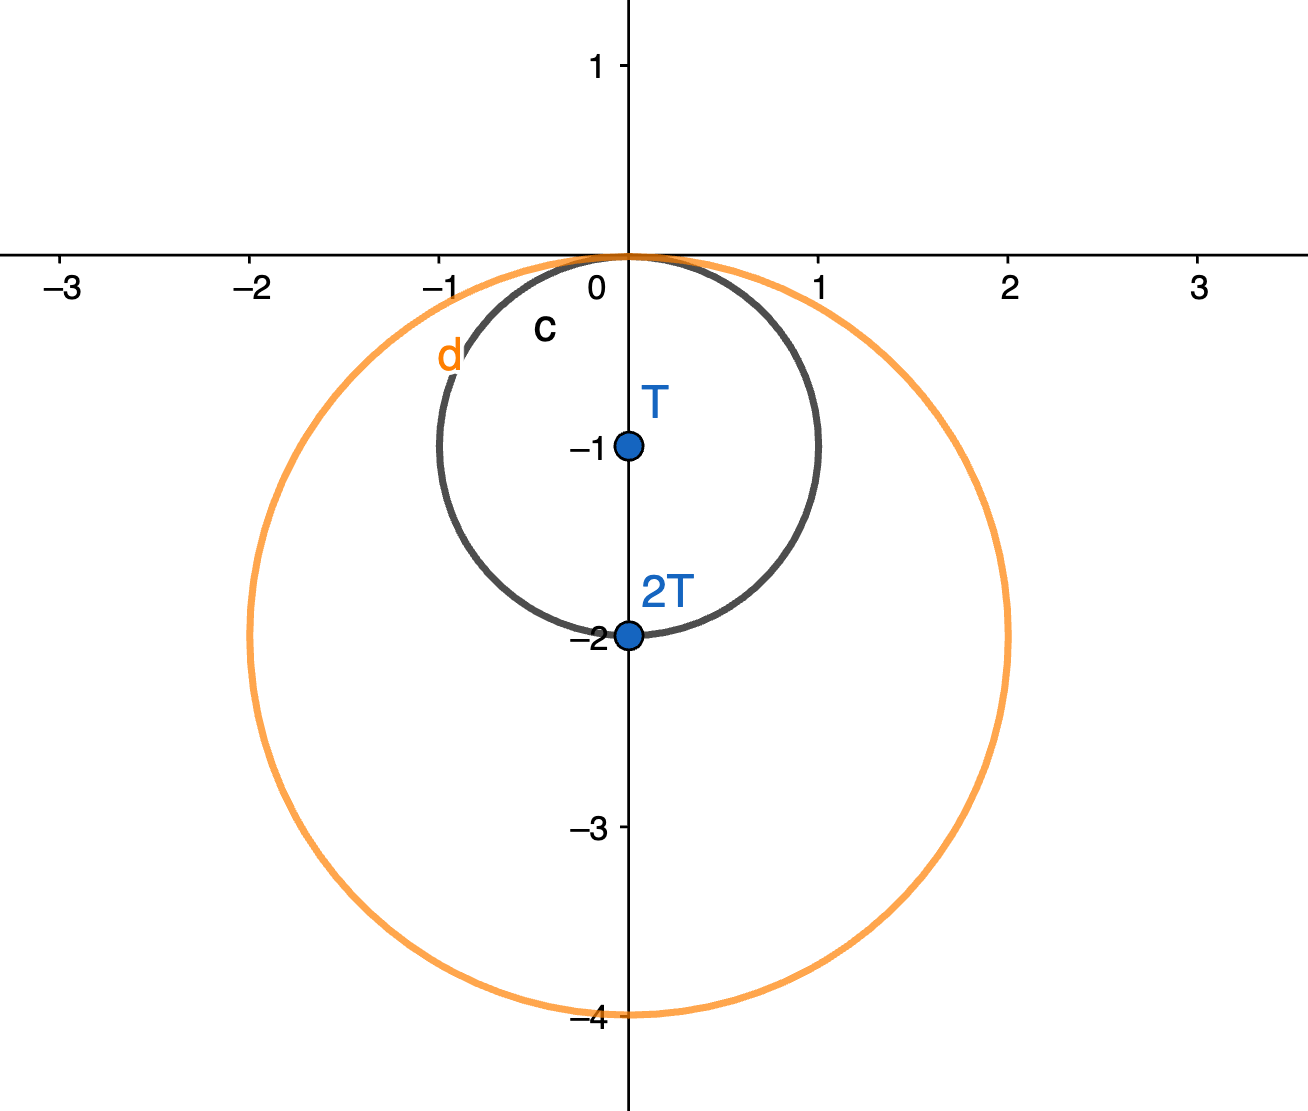
\includegraphics[scale=1]{image1.png}
	\end{figure}
	\end{center}
	
	 Define $f:B'_1(t)\setminus\{2t\}\rightarrow \Hs^n $ by
	\[
	f(x)=\frac{4(x-2t)}{\|x-2t\|^2}+2t,
	\]
	where $\Hs^n=\{(x_1,\cdots,x_n)\in \R^n:x_n\geq 0\}$. Notice that if $a=(a_1,\cdots,a_n)\in B'_1(t)$, then $a_1^2+\cdots +a_{n-1}^2+(a_n+1)^2\leq 1$. Assume that $f(x)=(f_1(x),\cdots,f_n(x))$, then because
	\[
	f(x)=\frac{4(x_1,\cdots,x_{n-1},x_n+2)}{x_1^2+\cdots +x_{n-1}^2+(x_n+2)^2}+2(-1,0,\cdots,0),
	\]
	using the fact that $a\in B'_1(t)$, we have
	\begin{align*}
	f_n(x)&=\frac{4x_n+8}{x_1^2+\cdots +x_{n-1}^2+(x_n+2)^2}-2\\
	&= \frac{4x_n+8}{x_1^2+\cdots +x_{n-1}^2+(x_n+1)^2+2x_n+3}-2\\
	&\geq\frac{4x_n+8}{2x_n+4}-2\\
	&=0.
	\end{align*}
	So $f(x)\in \Hs^n$ whenever $x\in B'_1(t)$. In the equations above, the denominator is nonzero because $x\neq 2t$. Now	we will show that $f$ is a homeomorphism. For $x,y\in B'_1(t)\setminus\{2t\}$, if $f(x)=f(y)$, then we have 
	\[
	\frac{4(x-2t)}{\|x-2t\|^2}=\frac{4(y-2t)}{\|y-2t\|^2}.\quad (1)
	\]
	Take the Euclidean norm both side gives
	\[
	\frac{4}{\|x-2t\|^2}=\frac{4}{\|y-2t\|},
	\]
	which yields $\|x-2t\|=\|y-2t\|$. Replace $\|x-2t\|$ by $\|y-2t\|$ to (1), one can easily check that we get
	\[
	x-2t=y-2t,
	\] 
	so $x=y$, which means $f$ is injective. For the surjective part, we first calculate the inversion of $f$. Because
	\begin{align*}
	f(f(x))&=\frac{4(f(x)-2t)}{\|f(x)-2t\|^2}+2t\\
	&=\frac{\frac{16(x-2t)}{\|x-2t\|^2}}{\left\|\frac{4(x-2t)}{\|x-2t\|^2}\right\|^2}+2t\\
	&=(x-2t)+2t\\
	&=x.
	\end{align*}
	Therefore, $f^{-1}(x)=f^{-1}(f(f(x)))=f(x)$. Now, to show that $f$ is surjective, we will show that $f^{-1}(x)\in B'_1(t)$ for all $x\in \Hs^n$. Indeed, for $x=(x_1,\cdots,x_n)\in \Hs^n$, we have 
	\begin{align*}
	\|f^{-1}(x)-t\|^2 &= \left\| \frac{4(x-2t)}{\|x-2t\|^2}+t \right\|^2\\
	&= \left\| \frac{4(x-2t)}{\|x-2t\|^2}\right\|^2 +\|t\|^2+2\left\langle{\frac{4(x-2t)}{\|x-2t\|^2},t}\right\rangle\\
	&= \frac{16\|x-2t\|^2}{\|x-2t\|^4}+1+\frac{8}{\|x-2t\|^2}\langle{x-2t,t}\rangle\\
	&=\frac{16}{\|x-2t\|^2}+1+\frac{8}{\|x-2t\|^2}\langle{(x_1,\cdots,x_n+2),(0,\cdots,0,-1)}\rangle\\
	&=\frac{16}{\|x-2t\|^2}+1+\frac{8(-x_n-2)}{\|x-2t\|^2}\\
	&=\frac{16-8x_n-16}{\|x-2t\|^2}+1\\
	&=\frac{-8x_n}{\|x-2t\|^2}+1\\
	&\leq 1
	\end{align*}
	because $x_n\geq 0$. (Wow. "Beautiful". I can spend all day doing these calculations.) So $f^{-1}(x)\in B'_1(t)\setminus\{2t\}$, which implies $f$ is a bijection. By the formula of $f(x)$ and $f^{-1}(x)$, we can see that both functions are continuous. Therefore, $f$ is a homeomorphism from $B'_1(t)\setminus \{2t\}\rightarrow \Hs^n$. So, for any point $a\in B'_1(t)$ that is not $2t$, $B'_1(t)\setminus\{2t\}$ is a neighborhood of $a$ that is homeomorphic to $\Hs^n$. If that point is $2t$, a simple rotation is enough to show that there is a neighborhood of $2t$ that is homeomorphic to $\Hs^n$. So a closed ball in $\R^n$ is an $n$-manifold with boundary. 
	
	Now, to show that is complement of every open ball is an $n$-manifold with boundary, we will reuse the function above. Let $g:\R^n\setminus\{2t\}\rightarrow\R^n$ defined by 
	\[
	g(x)=\frac{4(x-2t)}{\|x-2t\|^2}+2t,
	\]
	we will show that $g$ is a bijection. Notice that in the proof of injective of $f$, we don't use the domain. Thus similarly, we get $g$ is injective. And the proof of $g$ is surjective is by obviousness, we get $g$ is a bijection from $\R^n\setminus \{2t\}$ to $\R^n$. 
	
	Next, we will show that the boundary of the open ball $B'_1(t)$ is map to the the boundary of $\Hs^n$ (and $2t$ isn't counted of course). Indeed, if $\|x-t\|^2=1$, then 
	\begin{align*}
	\|x-2t\|^2&=\|x-t\|^2+\|t\|^2-2\langle{x-t,t}\rangle\\
	&=1+1-2\langle{(x_1,\cdots,x_n+1),(0,\cdots,0,-1)}\rangle\\
	&= 2+2(x_n+1)\\
	&=2x_n+4.
	\end{align*}
	Therefore, 
	\begin{align*}
	g(x)&=\frac{4(x-2t)}{\|x-2t\|^2}+2t\\
	&=\frac{4(x-2t)}{2x_n+4}+2t.
	\end{align*}
	Notice that 
	\[
	g_n(x)=\frac{4(x_n+2)}{2x_n+4}-2=2-2=0,
	\]
	we get $g$ maps $\partial B'_1(t)\setminus\{2t\}$ to $\partial\Hs^n$ Conversely, if $x\in\partial\Hs^n$, then $x$ has the form $(x_1,\cdots,x_{n-1},0)$. So
	\begin{align*}
	\|g^{-1}(x)-t\|^2&=\left\|\frac{4(x-2t)}{\|x-2t\|^2}+t\right\|^2\\
	&=\left\|\frac{4(x-2t)}{\|x-2t\|^2}\right\|^2+\|t\|^2+\frac{8}{\|x-2t\|^2}\langle{x-2t,t}\rangle\\
	&=\frac{16}{\|x-2t\|^2}+1+\frac{8}{\|x-2t\|^2}\langle{(x_1,\cdots,x_{n-1},2),(0,\cdots,0,-1)}\rangle\\
	&=\frac{16}{\|x-2t\|^2}+1+\frac{8}{\|x-2t\|^2}(-2)\\
	&=1.
	\end{align*}
	So the inverse of $g$ maps $\partial\Hs^n$ to $\partial B'_1(t)\setminus\{2t\}$. This implies $g$ is a bijection from $\partial B_1(t)\setminus\{2t\}$ to $\partial\Hs^n$. Therefore, $g$ is also a bijection from $H^n\setminus (B_1(t)\cup\{2t\})$ to $\{x=(x_1,\cdots,x_n)\in\R^n:x_n\leq 0\}$. But both $g$ and $g^{-1}$ are continuous, thus $g$ is homeomorphism from $H^n\setminus (B_1(t)\cup\{2t\})$ to $\{x=(x_1,\cdots,x_n)\in\R^n:x_n\leq 0\}$. So, for any $x$ in the compliment of $B_1(t)$ that is not $2t$, $H^n\setminus (B_1(t)\cup\{2t\})$ is a neighborhood of $x$ that is homeomorphic to $\{x=(x_1,\cdots,x_n)\in\R^n:x_n\leq 0\}$, which is homeomorphic to $\Hs^n$. If $x=2t$, by a simple rotation, we deduce to the case above. Therefore, the compliment of an open ball is an $n$-manifold with boundary.
	
	Now, for a general closed ball in $\R^n$, we will claim without proof (since the proof is already 3 pages fucking long) that there is a homeomorphism that map this ball to $B'_1(t)$. Similar for the compliment case, I'm too lazy now!
	
	For the manifold boundary equals the topological boundary part, as we show above, $g$ is a bijective from $\partial B'_1(t)\setminus\{2t\}$ to $\partial\Hs^n$. So with the similar argument as before, we get the manifold boundary equals the topological boundary.
	\end{proof}

\begin{problem}{3-5}
Show that a finite product of open maps is open; give a counterexample to show that a finite product of closed maps need not be closed.
\end{problem}
	\begin{proof}
	
	\end{proof}
	
\pagebreak

\begin{problem}{3-6}
Let $X$ be the topological space. The diagonal of $X\times X$ is the subset $\Delta=\{(x,x):x\in X\}\subset X\times X$. Show that $X$ is Hausdorff if and only if $\Delta$ is closed in $X\times X$.
\end{problem}
	\begin{proof}
	If $X$ is Hausdorff, we will show that $X\times X\setminus\Delta$ is open in $X\times X$. Indeed, any point in $X\times X\setminus\Delta$ has the form $(a,b)$ where $a\neq b$. Using the Hausdorff property, there exists disjoint neighborhood $U_a$ and $U_b$ of $a$ and $b$. But then, $U_a\times U_b$ is a neighborhood of $(a,b)$ and $U_a\times U_b\cap \Delta=\varnothing$. (If $U_a\times U_b\cap \Delta\neq \varnothing$, assume that $c$ is in the intersection, then $(c,c)\in U_a\times U_b$, which implies $c\in U_a\cap U_b\neq\varnothing$.) Therefore, $U_a\times U_b\subset (X\times X\setminus\Delta)$, which yields $X\times X\setminus\Delta$ is open. So $\Delta$ is closed.
	
	Conversely, assume that $\Delta$ is closed in $X\times X$, then $X\times X\setminus \Delta$ is open. For any $a,b\in X$ and $a\neq b$, consider the point $(a,b)\in X\times X\setminus\Delta$. By the definition of the product basis, there exists $U_a\times U_b\subset X\times X\setminus \Delta$ contains $(a,b)$, where $U_a$ and $U_b$ are open sets in $X$. But then $U_a$ and $U_b$ are disjoint neighborhood of $a$ and $b$, which implies $X$ is Hausdorff.
	\end{proof}

\begin{problem}{3-8}
Let $X$ denote the Cartesian product of countably many copies of $\R$ (which is just the set of all infinite sequences of real numbers), endowed with the box topology. Define a map $f:\R\rightarrow X$ by $f(x)=(x,x,\cdots)$ with the box topology. Show that $f$ is not continuous, even though each of its component functions is.
\end{problem}
	\begin{proof}
	To prove that each component function is continuous, without loss of generality, we will show that $f_1(x)=\pi_1\circ f(x)$ maps $x\mapsto x$, where $\pi_1$ is the canonical map of the first entry, is continuous. But this is just the identity map on $\R$, thus $f_1(x)$ is continuous. However, $f$ is not continuous because let $U_i=(-1-\frac{1}{i},1+\frac{1}{i})$ an open set in $\R$, then by the definition of the box topology, $\Pi_{i\in \N}U_i$ is open. But
	\[
	f^{-1}(\Pi_{i\in \N}U_i)=\bigcap_{i\in\N}f^{-1}(U_i)=[-1,1]
	\]
	which is closed. Therefore, $f$ is not continuous. 
	\end{proof}
	Wow, a great counter example!
\pagebreak

\begin{problem}{3-10}
Prove Theorem 3.41 (the characteristic property of disjoint union spaces).
\end{problem}
	\begin{proof}
	First, we will show that the disjoint union topology satisfy the characteristic property. If $f:\coprod_{\alpha\in A}X_\alpha \rightarrow Y$ is continuous, then for any open set $U$ in $Y$, we have 
	\[
	f^{-1}_\alpha(U)=f^{-1}(\iota_\alpha^{-1}(U)).
	\]
	But $\iota_\alpha^{-1}(U)$ is open by the definition of disjoint union topology, we get $f_\alpha = \iota_\alpha\circ f:X_\alpha\rightarrow Y$, the restriction of $f$ on $X_\alpha$, is continuous. Conversely, if $f_\alpha:X_\alpha\rightarrow Y$ is continuous for all $\alpha\in A$, then for all open sets $U\in Y$, we have
	\[
	f^{-1}(U)=\bigcup_{\alpha\in A}f_\alpha^{-1}(U).
	\]
	But an arbitrary union of open balls is open, thus $f$ is continuous.
	
	Now we will prove that the disjoint union topology is unique. Assume that $\T_1$ is a topology that satisfy the characteristic property, let $X=\coprod_{\alpha\in A}X_\alpha$ and $\T$ be the disjoint union topology. Because the identity map $(X,\T_1)\rightarrow (X,\T_1)$ is continuous, using the characteristic property, we get the restriction map $X_\alpha\rightarrow (X,\T_1)$ is continuous. This is saying, if $U$ is in $\T_1$, then its intersection with $X_\alpha$ is open for all $\alpha\in A$. Therefore $\T_1\subset \T$. Moreover,  $f_\alpha:X_\alpha\rightarrow (X,\T_1)$ is continuous for all $\alpha\in A$ implies $f:(X,\T)\rightarrow (X,\T_1)$ is continuous. Therefore, $\T\subset \T_1$. So $\T=\T_1$, which means the topology that satisfy the characteristic property is unique.
	\end{proof}
	
\begin{problem}{3-11}
Proposition 3.62(d) showed that the restriction of a quotient map to a saturated open subset is a quotient map onto its image. Show that the "saturated" hypothesis is necessary, by giving an example of a quotient map $f:X\rightarrow Y$ and an open subset $U\subset X$ such that $f|_U:U\rightarrow Y$ is surjective but not a quotient map.
\end{problem}
	\begin{proof}
	Let $I=[0,1]\subset \R$ and $\sim$ be the single relation $0\sim 1$. Let $f:I\rightarrow I/\sim$ be a quotient map, we will show that, for $J=[0,1)$, $f|_J$ is surjective but not a quotient map. It is not hard to see that $J$ is open in $I$ and $f|_J$ is a bijective. If $f|_J$ is a quotient map, then because $[0,1/2)$ is an open saturated subset of $[0,1)$, we get $f|_J[0,1/2)$ is open in $I/\sim$. But $f$ is a quotient map, thus $f^{-1}(f|_J[0,1/2))$ is open in $I$. That is $[0,1/2)\cup \{1\}$ is open in $I$, which is false. So our assumption is wrong, or $f|_J$ is not a quotient map.
	\end{proof}
	
\pagebreak

\begin{problem}{3-12}
Suppose $X$ is a topological space and $(X_\alpha)_{\alpha\in A}$ is an indexed family of topological spaces.
\begin{enumerate}[label=(\alph*)]
\item For any subset $S\subset X$, show that the subspace topology on $S$ is the coarsest topology for which $\iota_S:S\rightarrow X$ is continuous.
	\begin{proof}
	Let $\T$ be the subspace topology of $S$ and $\T'$ be a topology of $S$ such that $\iota_S:(S,T')\rightarrow X$ is continuous, then for the identity map $I:(S,\T')\rightarrow (S,\T)$, we have $\iota_S\circ I:(S,\T')\rightarrow X$ is continuous. Using the characteristic property of the subspace topology, we get $I$ is continuous, which yields $\T\subset \T'$. So $\T$ is the coarsest topology for which $\iota_S:S\rightarrow X$ is continuous.
	\end{proof}
	
\item Show that the product topology is the coarsest topology on $\prod_{\alpha\in A}X_\alpha$ for which every cononical projection $\pi_\alpha:\prod_{\alpha\in A}X_\alpha\rightarrow X_\alpha$ is continuous.
	\begin{proof}
	Let $\T$ be the cross product topology on $X=\prod_{\alpha\in A}X_\alpha$ and $\T'$ be a topology on $X$ such that $\pi_\alpha:X\rightarrow X_\alpha$ is continuous for all $\alpha\in A$. Let $I: (X,\T')\rightarrow (X,\T)$ be the identity map, then we have $\pi_\alpha\circ I: (X,\T')\rightarrow X_\alpha$ is continuous for all $\alpha\in A$. Using the characteristic property of the product topology, we get $I$ is continuous, that is $\T\subset \T'$.
	\end{proof}

\item Show that the disjoint union topology is the finest topology on $\coprod_{\alpha\in A}X_\alpha$ for which every canonical injection $\iota_\alpha:X_\alpha\rightarrow\coprod_{\alpha\in A} X_\alpha$ is continuous.
	\begin{proof}
	Let $\T$ be the disjoint union topology on $X=\coprod_{\alpha\in A}X_\alpha$ and $\T'$ be a topology on $X$ such that every canonical injection is continuous. Let $I$ be the identity map from $(X,\T)$ to $(X,\T')$. By the construction of $\T'$, we have $I|_{X_\alpha}:X_\alpha\rightarrow (X,\T')$ is continuous for all $\alpha\in A$. By the characteristic of the disjoint union topology, we get $I:(X,\T)\rightarrow (X,\T')$ is continuous. So $\T'\subset \T$, that is $T$ is the finest topology of $X$ such that every canonical injection is continuous.
	\end{proof}

\item Show that if $q:X\rightarrow Y$ is any surjective map, the quotient topology on $Y$ is the finest topology for which $q$ is continuous.
	\begin{proof}
	Let $\T$ be the quotient topology on $Y$ such that $q:X\rightarrow (Y,\T)$ is a quotient map, and $\T'$ be a topology on $Y$ for which $q:X\rightarrow (Y,T)$ is continuous. Let $I:(Y,\T)\rightarrow (Y,\T')$ be the identity map, then $I\circ q: X\rightarrow (Y,\T')$ is continuous. By the characteristic property of the quotient topology, $I:(Y,\T)\rightarrow (Y,\T')$ is continuous, which implies $\T'\subset \T$. So $\T$ is the finest topology for which $q$ is continuous.
	\end{proof}
\end{enumerate}
\end{problem}
\pagebreak

\begin{problem}{3-14}
Show that the real projective space $\mathbb{P}^n$ is an $n$-manifold.
\end{problem}
	\begin{proof}
	Let $R=\R^{n+1}\setminus\{0\}$, define a relation $\sim$ on $R$ by $x\sim y$ if there exists a $\lambda\in \R$ such that $x=\lambda y$. In Example 3.51, $\mathbb{P}^n$ is defined to be $R/\sim$. Consider the quotient map $p:R\rightarrow R/\sim$, because $R$ is second countable, we want to show that $R/\sim$ is locally Euclidean. Let $a=(a_1,\cdots,a_{n+1})\in R$, we will show that there is a neighborhood of $a$ that is homeomorphic to an open set in $\R^n$. Because $0\notin R$, there is at least one entry of $a$ that is nonzero. Without loss of generality, assume that $x_1\neq 0$. Let $U_1=\{x=(x_1,\cdots,x_{n+1})\in R:x_1=1\}$, it's not hard to see that $U_1$ is homeomorphic to $\R^n$. Now we will consider the map $p|_{U_1}$.
	
	Let $u\in U_1$, if $p|_{U_1}(u)=(0,\cdots)$, then there exists $\lambda\in \R^*=\R\setminus\{0\}$ such that $\lambda (1,\cdots) =\lambda u=(0,\cdots)$, contradiction. So $p|_{U_1}:U_1\rightarrow \mathbb{P}^n\setminus \{x_1=0\}$. For $u,v\in U_1$, if $p(u)=p(v)$, then $u=\lambda v$ for some $\lambda$. But the first entries of $u$ and $v$ are $1$, so $\lambda =1$ or $u=v$. Hence, $p$ is injective. Moreover, any element of $\mathbb{P}^n\setminus \{x_1=0\}$ has the form $p(u)$ where $u=(u_1,\cdots)\in R$. But we have $\frac{u}{u_1}\in U_1$ and $p(\frac{u}{u_1})=p(u)$, so $p$ is surjective.
	
	Because $p$ is a quotient map, it is continuous, which implies $p|_{U_1}$ is continuous since the restriction of a continuous map is continuous. Now we will show that $p|_{U_1}$ is open. For any open set $U\subset U_1$, $q^{-1}(q(U))$ is a union of open rays in $\R^{n+1}$, thus $q(U)$ is open. But $U\subset U_1$, thus $q|_{U_1}(U)$ is open. So $q$ is a homeomorphism from $U_1\rightarrow \mathbb{P}^n\setminus\{x_1=0\}$.
	
	To complete our proof for the locally Euclidean property, we need to show that $\mathbb{P}^n\setminus\{x_1=0\}$ is open, thus it is a neighborhood of $a$. Indeed, we have $q^{-1}(\mathbb{P}^n\setminus\{x_1=0\})=q^{-1}(q(U_1))$, which is open by open rays, so $\mathbb{P}^n\setminus\{x_1=0\}=q(U_1)$ is open, which yields $\mathbb{P}^n$ is locally Euclidean.
	
	Because $R$ is second countable, and $\mathbb{P}^n$ is locally Euclidean, we get $\mathbb{P}^n$ is second countable. So all that left is to show that $\mathbb{P}$ is Hausdorff. Let $\F=\{(a,b)\in R\times R: p(a)=p(b)\}= \{(a,\lambda a)\in R\times R:\lambda\in \R^*\}$, it is sufficient to show that $\F$ is closed in $R\times R$. For any sequence $(x^{(k)},\lambda_kx^{(k)})\in \F$ and $(x^{(k)},\lambda_k x^{(k)})\rightarrow (x,y)\in R\times R$, we have $x^{(k)}\rightarrow x$ and $\lambda_k x^{(k)}\rightarrow y$. Since $x\neq 0$, without loss of generality, assume that $x_1\neq 0$.	Now consider the first entry of $x$, because $x_1^{(k)}\rightarrow x_1\neq 0$, $x_1^{(k)}$ will eventually nonzero. So there is a nonzero subsequence of $(x_1^{(k)})$, to avoid complicated notations, we will assume that $x_1^{(k)}$ is nonzero, thus $\frac{1}{x_1^{(k)}}\rightarrow \frac{1}{x}$. Now consider the first entry of $y$, we have $\lambda_k x_1^{(k)}$ is convergent, thus $\lambda_k x_1^{(k)}\cdot \frac{1}{x_1^{(k)}} = \lambda_k$ is convergent. Let $\lambda_k\rightarrow \lambda$, then we get $\lambda_k x^{(k)}\rightarrow \lambda x=y$. So $(x,y)\in \F$ which yields $\F$ is closed. Therefore, $\mathbb{P}^n$ is a manifold.
	\end{proof}
	Open ray is a silly argument, tho it is short. So when I write open rays, I mean our discussion yesterday.

\begin{problem}{3-16}
Let $X$ be the subset $(\R\times \{0\})\cup (\R\times \{1\})\subset \R^2$. Define an equivalent relation on $X$ by declaring $(x,0)\sim (x,1)$ if $x\neq 0$. Show that the quotient space $X/\sim$ is locally Euclidean and second countable, but not Hausdorff.
\end{problem}
	\begin{proof}
	First, we will show that $X/\sim$ is locally Euclidean. Let $q: X\rightarrow X/\sim$ be a quotient map, and define $f:(X/\sim) \rightarrow \R$ maps $q(x,0)$ and $q(x,1)$ to $x$. Any element of $X/\sim$ has the form $q(x,0)$ or $q(x,1)$. If $x\neq 0\in \R$, then there exists an open neighborhood of $x$ that doesn't contain $0$, say $(a,b)$. Now we will show that $Q=\{q(x,0):x\in (a,b)\}$ is open in $(X/\sim)$. Indeed, $q^{-1}(Q)=\{q^{-1}(q(x)):x\in (a,b)\}=(a,b)\times\{0\}\cup (a,b)\times \{1\}$ which is open in $(\R\times \{0\})\cup (\R\times \{1\})$, so $Q$ is open. Since $q(x,1)=q(x,0)\in Q$, this is a neighborhood of $q(x,1)=q(x,0)$. Next, we will show that $f|_Q:Q\rightarrow f(Q)=(a,b)\subset \R$ is a homeomorphism. For any $q(u,0),q(v,0)\in Q$, $f|_Q(u)=f|_Q(v)$, implies $u=v$. So $f|_Q$ is one to one. For any open set $U\subset (a,b)$, $f|_Q^{-1}(U)= \{q(x,\epsilon):x\in U, \epsilon\in\{0,1\}$, which is open because $q^{-1}(f|_Q^{-1}(U))=(U\times\{0\})\cup (U\times\{1\})$ is open in $(\R\times \{0\})\cup (\R\times \{1\})$. So $f|_Q$ is continuous. Moreover, because $Q$ is open, a set $V\subset Q$ is open in $Q$ if and only if $V$ is open in $X/\sim$, that is $q^{-1}(V)=(V'\times \{0\})\cup (V'\times \{1\})$ is open in $X$. But this implies $f|_Q(V)=V'$ is open in $\R$. So $Q$ is homeomorphic to an open set in $\R$.
	
	Now consider $q(0,0)$, let $P=\{q(x,0):x\in (-1,1)\}\subset X/\sim$. Because $q^{-1}(P)=((-1,1)\times\{0\})\cup ((-1,0)\times 1)\cup((0,1)\times \{1\})$, which is a union of 3 open sets thus open, we get $P$ is open in $X/\sim$. Let $g:P\rightarrow (-1,1)\subset \R$ maps $q(x,0)\mapsto x$, we will show that $g$ is a homeomorphism. We can see $g$ is one to one and surjective by the definition of $g$. For any open set $E\subset (-1,1)$, we have $g^{-1}(E)=q(E\times\{0\})$. But this set is open because 
	\[
	q^{-1}(q(E)\times\{0\})=[(E\times\{0\})\cup (E\times\{1\})]\setminus \{(0,1)\}
	\]
	is open in $X$. So $g$ is continuous. Moreover, any open set of $P=q((-1,1)\times \{0\}$ has the form $q(O\times \{0\})$ where $O$ is open in $\R$. Thus $g(q(O\times \{0\}))=O$ is open in $\R$, which means $P$ is a coordinate neighborhood of $q(0,0)$. Similarly for the case $q(0,1)$, we conclude that $X/\sim$ is locally Euclidean.
	
	Since $\R^2$ is second countable, we get $X\subset \R^2$ is second countable. Moreover, any neighborhood of $q(0,0)$ has the form $q(V_0\times \{0\})$ where $V_0$ is a neighborhood of $0$ in $\R$, and any neighborhood of $q(0,1)$ has the form $q(V_1\times \{0\})$ where $V_1$ is a neighborhood of $0$ in $\R$. But then $V_0\cap V_1$ is a nonempty neighborhood of $0$, thus contain an $\epsilon\neq 0$. So $q(\epsilon,0)\in  q(V_0\times \{0\})\cap q(V_1\times \{0\})\neq \varnothing$. So $X/\sim$ is not Hausdorff.
	\end{proof}

\begin{problem}{3-18}
Let $A\subset \R$ be the set of integers, and let $Y$ be the quotient space $\R/A$ obtained by collapsing $A$ to a point.
\begin{enumerate}[label=(\alph*)]
\item Show that $Y$ is homeomorphic to a wedge sum of countable infinitely many circles.
	\begin{proof}
	Let $I=[0,1]\subset \R$ and $q:I\times N\rightarrow (I\times \N)/(\{0,1\}\times \N)$ be a quotient map that collapses $\{0,1\}\times\N$ to a point. For any $n\in\N$, notice that $q$ maps $I\times\{n\}\mapsto (I\times\{n\})/(\{0,1\}\times\{n\})$ and the codomain is homeomorphic to $\mathbb{S}^1$ by example 3.76. But $q(0,n)=q(1,n)$ is a point of $\mathbb{S}^1$ and $q(\epsilon_0,n_0)$ are all the same for $\epsilon_0\in\{0,1\}$ and $n_0\in \N$, so $q(I\times \N)$ is homeomorphic to the infinite countable wedge sum of $\mathbb{S}^1$.
	
	Now we will show that $q(I\times N)$ is homeomorphic to $\R/A$. Let $p:\R\rightarrow \R/A$ be a quotient map and $f:X=(I\times\N)/(\{0,1\}\times\N)\rightarrow \R/A$ maps $q(x,n)\rightarrow p(x+n)$, where $x\in I$ and $n\in \N$. If $f(q(x_1,n_1))=f(q(x_2,n_2))$, then $p(x_1+n_1)=p(x_2+n_2)$. If $x_1+n_1\neq x_2+n_2$ then $x_1+n_1$ and $x_2+n_2$ are in $A$. But $n\in \N\subset A$, so $x_1,x_2\in A\cap I=\{0,1\}$, which yields $q(x_1,n_1)=q(x_2,n_2)$ by the definition of $q$. If $x_1+n_1=x_2+n_2$, then $|x_1-x_2|=|n_1-n_2|\in A$. Notice that $x_1,x_2\in I=[0,1]$ so the distance between $x_1$ and $x_2$ is at most $1$. If $|x_1-x_2|=1$, then $\{x_1,x_2\}=\{0,1\}$, which implies $q(x_1+n_1)=q(x_2+n_2)$. If $|x_1-x_2|=0$, then $x_1=x_2$, which implies $n_1=n_2$. So $q(x_1,n_1)=q(x_2,n_2)$. In any case, we get $q(x_1,n_1)=q(x_2,n_2)$, so $f$ is injective.
	
	Any point in $\R/A$ has the form $p(x)=p((x-\lfloor{x}\rfloor)+\lfloor{x}\rfloor)=f(q((x-\lfloor{x}\rfloor),\lfloor{x}\rfloor)$ where $x\in \R$. So $f$ is surjective.
	
	Any open set in $\R/A$ has the from $p(U)$ where $U$ is an open saturated set in $\R$. We have $f^{-1}(p(U))=\{q(x,n):f(q(x,n))\in p(U)\}=\{q(x,n):p(x+n)\in p(U)\}$. But $U$ is saturated, thus $p(x+n)\in p(U)$ if and only if $x+n\in U$. So $f^{-1}(p(U))=\{q(x,n):x+n\in U\}$, which implies $q^{-1}\circ f^{-1}\circ p(U)=\{(x,n)\in I\times\N:x+n\in U\}$. For any $n_0\in\N$, it's not hard to see that the set $U-n_0=\{u-n_0:u\in U\}$ is open, therefore $q^{-1}\circ f^{-1}\circ p(U)\cap I\times \{n_0\} = (U-n_0,n_0)$ is open for all $n_0\in \N$. So $f^{-1}\circ p(U)$ is open in $X$, which yields $f$ is continuous.
	
	Lastly, any open set in $X$ has the form $q(V)$ where $V$ is an open saturated subset of $I\times \N$. We want to show that $p^{-1}(f(q(V)))$ is open in $\R$, thus $f(q(V))$ is open in $\R/A$. Notice that
	\begin{align*}
	p^{-1}\circ f\circ q(V)&=p^{-1}(\{p(x+n):x\in I, n\in\N,(x,n)\in V\})\\
	&=\{x+n:x\in I,n\in \N,(x,n)\in V\}.
	\end{align*}
	If $V\cap (\{0,1\}\times \N)=\varnothing$, then for all $n_0\in \N$, we have $V\cap (I\times \{n_0\})=V\cap [(0,1)\times\{n_0\}]$ is open in $I\times \N$. So $\{x+n_0:(x,n_0)\in V\cap (I\times \{n_0\})\}$ is open (this set is the set of adding $n_0$ to an open subset of $I$). Hence,
	\begin{align*}
	p^{-1}\circ f\circ q(V)&=\{x+n:x\in I,n\in \N,(x,n)\in V\} \\
	&=\bigcup_{n_0\in\N}\{x+n_0:x\in I,(x,n_0)\in V\}, 
	\end{align*}
	which is a union open sets, thus open. 
	
	If $V\cap (\{0,1\}\times \N)\neq \varnothing$, then because $V$ is a saturated set, we get $(\{0,1\}\times \N)\subset V$. Consider the set $K=\{x+n:x\in I,n\in \N,(x,n)\in V\}$. Any point of $K$ has the form $x_0+n_0$, where $x_0\in I$ and $n\in \N$. If $x_0\notin\{0,1\}$, then let $(x_0,n_0)\in V\cap (I\times\{n_0\})=B_1\times \{n_0\}$. Because $V$ is open in $I\times\N$, thus $B_1\times \{n_0\}$ is open in $I\times \{n_0\}$. This implies $B_1$ is open in $I$, so $x_0\in B_1\setminus\{0,1\}$ is open in $\R$ and $(B_1\setminus\{0,1\})+n_0\subset K$ is a neighborhood of $x_0+n_0$. If $x_0\in \{0,1\}$, then $x_0+n_0$ is in $\N$, with out loss of generality, assume that $x_0=1$, then $x_0+n_0=1+n_0=0+(1+n_0)$. Hence $(1,n_0),(0,n_0+1)\in V$. Now we will find a neighborhood of $1+n_0$ in $\R$ that is a subset of $K$. Using the same technique as above, let $V\cap (I\times\{n_0\})=B_2\times \{n_0\}$ and $V\cap (I\times\{1+n_0\})=B_3\times \{1\}$, then $1\in B_2$ and $0\in B_3$. Let $A_1=\{x+n_0:x\in I,x\in B_2\}= \{x+n:x\in I,n\in \N,(x,n)\in B_2\times\{n_0\}\}\subset K$ is an open subset of $[n_0,1+n_0]$. Similarly, we get $A_2=\{x+(n_0+1):x\in B_3\}\subset K$ is open in $[1+n_0,2+n_0]$. Because $1+n_0\in A_1\cap A_2$, the set $A_1\cup A_2$ is open in $[n_0,n_0+2]$. So $(A_1\cup A_2)\setminus\{n_0,n_0+2\}$ is a neighborhood of $n_0+1$ in $\R$ that is a subset of $K$. So $p^{-1}\circ f\circ q(V)$ is open in $\R$, which implies $f\circ q(V)$ is open in $\R/A$. So $f$ is an open map, and thus $f$ is a homeomorphism. 
	
	In conclusion, the wedge sum of countable infinitely many circle is homeomorphism to $X$, which is homeomorphism to $\R/A$.
	\end{proof}
\item Show that the equivalence class $A$ does not have a countable neighborhood basis in $Y$, so $Y$ is not first or second countable.
	\begin{proof}
	Let $p:\R\rightarrow \R/A$ be a quotient map and $x=p(A)$. A neighborhood of $x$ has the form $p(U)$ where $U$ is an open saturated subset of $p$ in $\R$ and $A\subset U$. Let $p(U)$ and $p(U')$ be two neighborhoods of $x$ such that $p(U)\subset p(U')$, then because $U$ and $U'$ are saturated, we have $U=p^{-1}(p(U))\subset p^{-1}(p(U'))=U'$. Let $\F=\{U\subset \R: U \text{ is open and } A\subset U\}$ be the family of open subsets of $\R$ that contains every integer, we will rephrase the problem as follow. For any sequence of set $U_n\in\F$, there exists $U\in\F$ such that $U_n\not\subset U$ for all $n\in\N$. Because if this is true, then for any countable neighborhood $p(U_n)$ of $x$, there is no $n_0\in \N$ such that $p(U_n)\subset p(U)$. This means $p(U_n)$ is not a neighborhood basis of $x$. So $Y$ is not first countable. 
	
	For any $n_0\in\N$ and $z\in A$, because $A\subset U_n$, there is an open ball of $z$ that is a subset of $U_n$. Let that ball be $(z-\epsilon_{n_0}(z),z+\epsilon_{n_0}(z))$, where $\epsilon_{n_0}:A\rightarrow (0,\frac{1}{2})$ (we let the values of these $\epsilon$ in $(0,\frac{1}{2})$ to avoid two different open balls collapse). Notice that if $U_n\subset U$, then
	\[
	\bigcup_{z\in A}(z-\epsilon_{n_0}(z),z+\epsilon_{n_0}(z))\subset U_n\subset U,
	\]
	our proof, which use contradiction, will shift focus onto this union of open balls. Let 
	\[
	\epsilon(z)=\frac{\epsilon_z(z)}{2}<\epsilon_z(z), \text{ for } z\geq 1
	\]
	and $\epsilon(z)=1/2$ otherwise. So for any $z\in \N$, we have $(z-\epsilon(z),z+\epsilon(z))$ is a strict subset of $(z-\epsilon_z(z),z+\epsilon_z(z))$. Let
	\[
	U=\bigcup_{z\in A}(z-\epsilon(z),z+\epsilon(z)),
	\]
	then for any $n_0\in \N$, we have $(n_0-\epsilon(n_0),n_0+\epsilon(n_0))\subset U$ is a strict subset of $(n_0-\epsilon_{n_0}(n_0),n_0+\epsilon_{n_0}(n_0))\subset U_{n_0}$, thus $U_{n_0}\not\subset U$. So $Y$ is not first countable, thus not second countable.
	\end{proof}
\end{enumerate}
\end{problem}

\begin{problem}{3-24}
Consider the action of $O(n)$ on $\R^n$ by matrix multiplication as in Example 3.88(b). Prove that the quotient space is homeomorphic to $[0,\infty)$.
\end{problem}
	\begin{proof}
	Let $q:\R^n\rightarrow \R^n/O(n)$ be the quotient map and $f:\R^n/O(n)\rightarrow [0,\infty)$ maps $O(n)\cdot x\mapsto \|x\|$. By Example 3.88(b), the orbits of the $O(n)$ action are $\{0\}$ and the spheres centered at $0$, we can easily see that $f$ is a bijection. Let $(a,b)$ be an open ball on $[0,\infty)$, then $f^{-1}(a,b)=\{O(n)\cdot x:\|x\|\in (a,b)\}$. Notice that $q^{-1}\circ f^{-1}(a,b)=\{x\in \R^n:\|x\|\in (a,b)\}$, which is open in $\R^n$, therefore, $f^{-1}(a,b)$ is open in $\R^n/O(n)$. Since the set of open balls is the basis for $[0,\infty)$, we get $f$ is continuous. Moreover, an open saturated subset of $q$ in $\R^n$ has the form $\{x\in \R^n:\|x\|\in U\}$ where $U$ is an open subset of $[0,\infty)$. So any open subset of $\R^n/O(n)$ has the form $B = \{O(n)\cdot x:\|x\|\in U\}$. But then $f(B)=U$ which is open, therefore $f$ is a homeomophism.
	\end{proof}
\subsection{Bonus Problem}

\begin{exercise}{1}
Show that the graph of a continuous map $f:\R^n\rightarrow \R^p$ is a $p$-manifold in $\R^{n+p}$.
\end{exercise}
	\begin{proof}
	The graph of $f$ in $\R^{n+p}$ has the form $(x,f(x))$ where $x\in \R^n$ and $f(x)\in\R^p$. It is sufficient to prove that the map $g:\R^n\rightarrow \R^{n+p}$ maps $x\rightarrow (x,f(x))$ is a homeomorphism. Indeed, if $x_n\rightarrow x$ in $\R^n$, then because $f$ is continuous, we have $f(x_n)\rightarrow f(x)$. Therefore, $(x_n,f(x_n))\rightarrow (x,f(x))$. Conversely, any convergent sequence in the graph of $f$ has the form $(x_n,f(x_n))\rightarrow (x,f(x))$ for some $x_n$ and $x\in \R^n$. Therefore, we have $x_n\rightarrow x$. So $g$ is a homeomorphism, which means the graph of $f$ is a $p$-manifold.
	\end{proof}
	
\begin{exercise}{2}
Show that the disjoint union of uncountably many copies of R is locally Euclidean of dimension 1, Hausdorff, but not second countable.
\end{exercise}
	\begin{proof}
	Because $\R$ is locally Euclidean, Hausdorff, and second countable, by exercise 3.43, the disjoint union of $\R$'s is Hausdorff and locally Euclidean. Moreover, this is an uncountable many copies of $\R$, exercise 3.43 (d) implies this union is not second countable.
	\end{proof}
	Is there a good reason why you assign this exercise? Cause it's quiet obvious to me :))
	
\section{Chapter 4}
\subsection{Exercise}
	
\begin{exercise}{4.3}
	Suppose $X$ is a connected topological space, and $\sim$ is an equivalence relation on $X$ such that every equivalence class is open. Show that there is exactly one equivalence class, namely $X$ itself.
\end{exercise}
	\begin{proof}
	Let $q:X\rightarrow X/\sim$ is the quotient map, then every equivalence class is open means every saturated subset of $q$ is open in $X$. Let $A\subset X$ be a nonempty saturated subset of $X$, then by the hypothesis, $A$ is open. However, $X\setminus A$ is also a saturated subset of $X$ thus open, which implies $A$ is clopen in $X$. But $X$ is connected and $A$ is nonempty, we get $A=X$. So $X$ is the only equivalence class.
	\end{proof}

\begin{exercise}{4.4}
Prove that a topological space $X$ is disconnected if and only if there exists a nonconstant continuous function from $X$ to the discrete space $\{0,1\}$.
\end{exercise}
	\begin{proof}
	If $X$ is disconnected, then there exist two disjoint, nonempty, open covers $A,B$ of $X$. Let $f:X\rightarrow\{0,1\}$ maps $f(A)\mapsto \{0\}$ and $f(B)\mapsto\{1\}$. There are only four open subsets of $\{0,1\}$, which are $\{\{0\},\{1\},\varnothing,\{0,1\}\}$, and their inverse images are $\{A,B,\varnothing,X\}$ respectively. Since all the inverse images are open in $X$, we get $f$ is continuous.
	
	If $X$ is connected, then by the Proposition 4.2, every continuous function from $X$ to a discrete space is a constant. Thus there is no nonconstant continuous function from $X$ to $\{0,1\}$.
	\end{proof}

\begin{exercise}{4.5}
Prove that a topological space is disconnected if and only if it is homeomorphic to a disjoint union of two or more nonempty spaces.
\end{exercise}
	\begin{proof}
	If $X$ is a disconnected topological space, then $X=A\cup B$ where $A$ and $B$ are two nonempty, disjoint, open subset of $X$. Let $A$ and $B$ be spaces with the subspace topology, we will show that the identity map $f:X\rightarrow A\coprod B$ is a homeomorphism. Indeed, if $U$ is open in $X$, then $U\cap A$ and $U\cap B$ are open in $A$ and $B$ respectively, therefore $f(U)$ is open in $A\coprod B$. Moreover, if $V$ is open in $A\coprod B$, then $f^{-1}(V)$ is open in $A$ and in $B$. But $A$ and $B$ are open, thus $f^{-1}(V)\cap A$ and $f^{-1}(V)\cap B$ are open in $X$. Therefore 
	\[
	f^{-1}(V) = f^{-1}(V)\cap X=f^{-1}(V)\cap (A\cup B)=(f^{-1}(V)\cap A)\cup (f^{-1}(V)\cap B)
	\]
	is open in $X$ as a union of two open sets. So $f$ is a homeomorphism.
	
	If $X$ is homeomorphic to $\coprod_{i\in T}X_i$, where $\T$ is an index set and $X_i$ are nonempty spaces, then obviously $X_1$ and $X_1^c$ are open in $\coprod_{i\in T}X_i$ with $1\in T$. So $X_1$ is clopen in $\coprod_{i\in T}X_i$. Now, let $g:X\rightarrow \coprod_{i\in T}X_i$ be a homeomorphism, then $g^{-1}(X_1)$ is a clopen set in $X$. Because $X_i$ are nonempty for all $i\in T$, we get $g^{-1}(X_1)$ is neither $\varnothing$ nor $X$, which means $X$ is disconnected.
	\end{proof}
	
\begin{exercise}{4.10}
Suppose $M$ is a connected manifold with nonempty boundary. Show that its double $D(M)$ is connected.
\end{exercise}
	\begin{proof}
	Let $q:M\coprod M\rightarrow M\cup_{\partial M}M=D(M)$ be the quotient map. Because $q$ is continuous, we get $q(M)$ is a connected space. But $D(M)$ is a union of two connected subspaces with nonempty intersection, thus by Proposition 4.9(d), $D(M)$ is connected.
	\end{proof}
	
\begin{exercise}{4.14}
Prove that
\begin{enumerate}[label=(\alph*)]
\item Every continuous image of a path connected image is path connected.
	\begin{proof}
	Let $X$ be a path connected space and $f:X\rightarrow f(X)$ be a continuous. Any two points in $f(X)$ has the forms $f(a)$ and $f(b)$ where $a,b\in X$. But $X$ is path connected, there exists a continuous map $g:I\rightarrow X$ where $g(0)=a$ and $g(1)=b$. So $f\circ g:I\rightarrow f(X)$ is a continuous map that map $0\mapsto f(a)$ and $1\mapsto f(b)$. So $f(X)$ is path connected.
	\end{proof}
\item Let $X$ be a space, and let $\{B_\alpha\}_{\alpha\in A}$ be a collection of path connected subspaces of $X$ with a point in common. Then $\bigcup_{\alpha \in A}B_\alpha$ is path connected.
	\begin{proof}
	For any two points $a,b\in\bigcup_{\alpha\in A}B_\alpha$, if $a,b\in U_\alpha$ for some $\alpha_0\in A$, then there exists a continuous map from $I\rightarrow B_{\alpha_0}\subset\bigcup_{\alpha\in A}B_\alpha$ where $0\mapsto a$ and $1\mapsto b$. If such $\alpha_0$ doesn't exists, assume that $a\in U_1$ and $b\in U_2$ and $x\in U_1\cap U_2$. Because $U_i$ is continuous for all $i\in A$, there exists a continuous map $g_1:I\rightarrow U_1$ and $g_2:I\rightarrow U_2$ such that $g_1(0)=a,g_1(1)=g_2(0)=x,g_2(1)=b$. So $g:I_1\coprod I_2\rightarrow \bigcup_{\alpha\in A}B_\alpha$ that map $x\mapsto g_1(x)$ if $x\in I_1$ and $x\mapsto g_2(x)$ if $x\in I_2$ is continuous by the characteristic property of disjoint union topology. Here, $I_1, I_2$ are homeomorphic to $[0,1]$ with $h:[0,1]\rightarrow I_1$ and $k:[0,1]\rightarrow I_2$ are homeomorphisms. Notice that $g_1(h(1))=g_2(k(0))$, define a single relation $h(1)\sim k(0)$, and $I_1\vee I_2=I_1\coprod I_2/\sim$. Then $g$ is a continuous from $I_1\vee I_2$ to $\bigcup_{\alpha\in A}B_\alpha$. But $I_1\vee I_2$ is homeomorphic to $I$, thus $\bigcup_{\alpha\in A}B_\alpha$ is path connected.
	\end{proof}
\item Every product of finitely many path connected spaces is path connected.
	\begin{proof}
	We will prove for the product of 2 spaces, the general case is by mathematical induction. Assume that $X$ and $Y$ are path connected spaces, for $(a_1,a_2)$ and $(b_1,b_2)$ in $X\times Y$, there exist continuous maps $g_1:I\rightarrow X$ such that $g_1(0)=a_1$ and $g_1(1)=b_1$, and $g_2:I\rightarrow Y$ such that $g_2(0)=a_2$ and $g_2(1)=b_2$. By the characteristic property of product spaces, we get $g:I\rightarrow X\times Y$ maps $x\mapsto (g_1(x),g_2(x))$ is continuous such that $g(0)=(a_1,b_1)$, $g(1)=(a_2,b_2)$. So $X\times Y$ is connected.
	\end{proof}
\item Every quotient space of a path connected space is path connected.
	\begin{proof}
	Because quotient map is a continuous map, by part (a), the quotient space of a path connected space is path connected.
	\end{proof}

\end{enumerate}
\end{exercise}

\begin{exercise}{4.22}
Let $X$ be any space, show that
\begin{enumerate}[label=(\alph*)]
\item The path components of $X$ form a partition of $X$.
	\begin{proof}
	Let $A$ and $B$ be two different path components of $X$. If $A\cap B\neq \varnothing$, then by Proposition 4.13 (b), we get $A\cup B$ is path connected, contradict to the fact that $A$ is the maximal path connected set. So every path connected components are disjoint. Moreover, for all $x\in X$, we have $\{x\}$ is path connected, so the union of all path connected subsets that contain $\{x\}$ is a path component. So the path components cover $X$, which means they form a partition of $X$.
	\end{proof}
\item Each path component is contained in a single component, and each component is a disjoint union of path components.
	\begin{proof}
	Because a path component is a path connected set, thus connected, that set is contained in a single component. For a component $A$ of $X$, consider every path component $P_i$ such that $P_i\cap A\neq \varnothing$. Because the set of path components covers $X$, we $A\subset \bigcup P_i$. Moreover, every path component is contained in a single component, we get $\bigcup P_i\subset A$. Since $P_i$'s are disjoint, every component is a disjoint union of path components.
	\end{proof}
\item Any nonempty path connected subset of $X$ is contained in a single path component.
	\begin{proof}
	Assume that $A$ is a nonempty path component and $B$ be a nonempty path connected subset of $X$ such that $B\not\subset A$ and $B\cap A\neq \varnothing$. But this implies $A\cup B$ is strictly bigger that $A$ and it is path connected, which contradict the definition of path component. So every path connected subset of $X$ is contained in a single path component.
	\end{proof}
\end{enumerate}
\end{exercise}

\begin{exercise}{4.24}
Prove that every manifold is locally connected and path connected.
\end{exercise}
	\begin{proof}
	Let $M$ be an $n$-manifold. For any $x\in M$, there exists a neighborhood $V_x$ of $x$ that is homeomorphic to $\R^n$. But $\R^n$ is path connected and connected, thus $V_x$ is path connected and connected. This implies $M$ is locally connected and path connected.
	\end{proof}
	
\begin{exercise}{4.28}
Prove that if $X$ is any topological space, a subset $A\subset X$ is compact (in the subspace topology) if and only if every cover of $A$ by open subsets of $X$ has a finite subcover.
\end{exercise}
	\begin{proof}
	If every cover of $A$ by open subsets of $X$ has a finite subcover, then any open cover of $A\subset X$ has finite subcover because any subset of $A$ is a subset of $X$.
	
	Conversely, if $A$ is compact in the subspace topology, then for any open cover $U_{i}$ where $i\in I$, an index set, we get $U_i\cap A$ is an open cover of $A$ in $A$. By the compactness of $A$, there exists a finite subcover of $A$, namely $U_1\cap A,\cdots, U_n\cap A$. But then, $U_1,\cdots, U_n$ is a finite subcover of $A$. 
	\end{proof}
	
\begin{exercise}{4.29}
In any topological space $X$, show that every union of finitely many compact subsets of $X$ is compact.
\end{exercise}	
	\begin{proof}
	We first show that the union of $2$ compact subsets is compact. The finite case can be deduced from induction. 
	
	Let $A,B\subset X$ be two compact sets. For any open cover $U$ of $A\cup B$, $U$ also cover $A$ and $B$. So there exist open subcovers $U_1,\cdots, U_n$ of $A$ and $U_{n+1},\cdots,U_m$ of $B$ ($U_i$'s here are not necessarily distinct). Then $U_1,\cdots, U_m$ is an open subcover of $A\cup B$. So $A\cup B$ is compact.  
	\end{proof}

\begin{exercise}{4.37}
Suppose $M$ is a compact manifold with boundary. Show that the double of $M$ is compact.
\end{exercise}
	\begin{proof}
	Let $U_i$ be an open cover for $D(M)=M\cup_fM'$, where $M'$ is just another copy of $M$, then $U_i$ is also an open cover for $M$ and $M'$. So there exists a finite subcover for $M$ and $M'$. Their union is indeed a finite open cover for $D(M)$. So $D(M)$ is compact.
	\end{proof}


\begin{exercise}{4.38}
Let $X$ be a compact space, and suppose $\{F_n\}$ is a countable collection of nonempty closed subsets of $X$ that are nested, which means that $F_{n+1}\subset F_n$ for each $n$. Show that $\bigcap_n F_n$ is nonempty.
\end{exercise}
	\begin{proof}
	The proof is by mathematical contradiction. Assume that $\bigcap_nF_n=\varnothing$, then we would get $\{F_n^c\}$ is an open cover for $X$. Because $X$ is compact, it is has a finite subcover. Hence there exists $N>0$ such that
	\[
	\bigcup_{n\leq N}F_n^c=X.
	\]
	But this is impossible because $F_{N+1}\subset F_i$ for all $i<N+1$. Hence $\bigcup_{n\leq N}F_n^c\subset F_{N+1}^c$. But $F_{N+1}$ is nonempty, thus $F_{N+1}^c$ is strictly smaller than $X$, contradiction.
	\end{proof}

\begin{exercise}{4.49}
    Prove the preceding three theorems
    \begin{itemize}
        \item Every bounded sequence in $\R^n$ has a convergent subsequence,
        \item Endowed with the Euclidean metric, a subset of $\R^n$ is a complete metric space if and only if it is closed in $\R^n$. In particular, $\R^n$ is complete,
        \item Every compact metric space is complete.
    \end{itemize}
\end{exercise}
    \begin{proof}
        \hfill
        \begin{itemize}
            \item Any bounded sequence $(x_n)$ in $\R^n$ can be contained in a closed ball of $\R^n$, which is compact. Hence $(x_n)$ has a convergent subsequence.
            \item Let $A\subset \R^n$. If $A$ is complete, then any Cauchy sequence of $A$ is convergent in $A$. Thus $x_n\in A$ and $x_n\to x$ implies $x\in A$. Conversely, if $A$ is closed, then for any Cauchy sequence $x_n\in A$, because $\R^n$ is complete, there exists $x\in \R^n$ such that $x_n\to x$. But $A$ is closed, thus $x\in A$, which implies that $A$ is complete. (I have no idea why this theorem is in the compactness chapter.)
            \item Let $X$ be a compact metric space and $x_n$ be a Cauchy subsequence of $X$. Because $X$ is sequential compact, there is a subsequence of $x_n$ that converge to $x\in X$. But $(x_n)$ is Cauchy, thus $x_n\to x$. So $X$ is complete.
        \end{itemize}
    \end{proof}
	
\begin{exercise}{4.58}
Using the map of Example 4.55, show that there is a coordinate ball in $\set{S}^n$ whose closure is equal to all of $\set{S}^n$.
\end{exercise}
    \begin{proof}
        From Example 4.55, we see that $q:\overline{\mB}^n\to \mS^n$ is a quotient space, defined by $$q(x) = (2\sqrt{1-|x|^2}x, 2|x|^2-1).$$
        Let $\mB^n$ be the open ball of dimension $n$, because $q$ is a closed map, $q|_{\mB^n}$ is a closed map. We will now check that $q$ is injective. Let $x,y\in \mB^n$, if $q(x)=q(y)$, then the second entry implies that $$2|x|^2-1=2|y|^2-1.$$ Thus $|x|=|y|$. By the first entry, we get $$2\sqrt{1-|x|^2}x = 2\sqrt{1-|y|^2}y$$. But $x,y\in \mB^n$, therefore $|x|$ and $|y|$ are strictly smaller than $1$. So the equation above gives $x=y$.

        When $x\in \partial \overline{\mB}^n$, we get $|x|=1$. Hence, $q(x)=(0,1)$. So the boundary of $\overline{\mB}^n$ map to one point $(0,1)$. But $q$ is surjective, thus $q(\overline{\mB}^n)=\mS^n\setminus\{(0,1\}$. So by the closed Lemma, $q|_{\mB^n}\colon \mB^n\to \mS^n\setminus\{(0,1\}$ is a homeomorphism, that is, $\mB^n$ is homeomorphic to $\mS^n\setminus \{(0,1)\}$. So $\mS^n\setminus \{(0,1)\}$ is a coordinate ball. The colure of $\mS^n\setminus \{(0,1)\}$ must include itself, so it can be either $\mS^n$ or itself. The former is not closed because $\{(0,1)\}$ is not open, thus its closure is $\mS^n$.
    \end{proof}

\pagebreak

\begin{exercise}{4.61}
Complete the proof of Proposition 4.60 by showing that $\B$ is a basis.
\end{exercise}
    \begin{proof}
        Let $V$ be an arbitrary open subset of $M$, it is sufficient to show that $V$ is a union of some element of $\B$. This can be done by the following construction. For any $x\in V$, because $\{U_i\}$ covers $M$, there is some $i$ such that $x\in U_i$. Hence $\phi(x)\in \hat U_i$. Because $\hat U_i$ is open and the set of points of rational coordinate is dense in $\R^n$, there is a $y\in \R^n$ of rational coordinate and a rational $\epsilon>0$ such that $\varphi(x)\in B_\epsilon(y)$. (This part is kinda tedious, but such $y$ and $\epsilon$ can be found with no problem.) So $V_x:=\phi^{-1}(B_\epsilon(y))$ is an element of $\B$ that contains $x$ and is a subset of $V$. So 
        \[
        \bigcup_{x\in V}V_x = V.
        \]
        This prove that $\B$ is a basis for $M$.
        \begin{figure}[H]
            \centering
            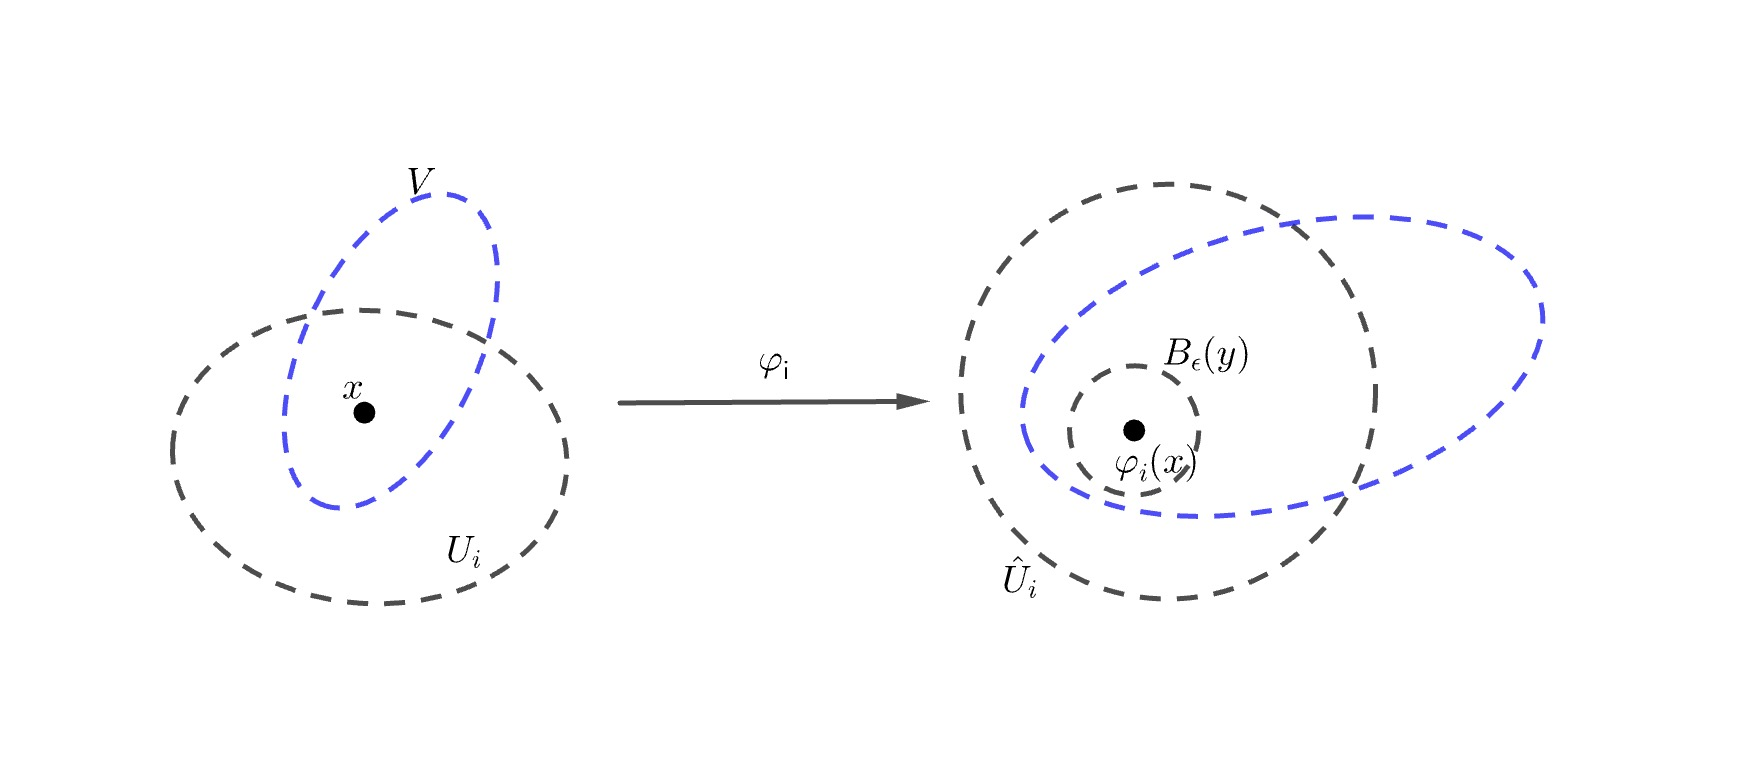
\includegraphics[scale = 0.3]{Topology-Lee/image5.jpg}
            \caption{Caption}
            \label{fig:enter-label}
        \end{figure}
    \end{proof}

\begin{exercise}{4.62}
Prove that every manifold with boundary has a countable basis consisting of regular coordinate balls and half-balls.
\end{exercise}
    \begin{proof}
        It should be exactly similar to the regular coordinate balls case.
    \end{proof}

\begin{exercise}{4.67}
    Show that any finite product of locally compact spaces is locally compact.
\end{exercise}
    \begin{proof}
        We will show that the cross product of $2$ locally compact spaces is locally compact. The finite case is by mathematical induction. Let $A$ and $B$ be locally compact. For any point $(a,b)\in A\times B$, there exists neighborhoods $V_a,V_b$ subsets of $U_a, U_b$, which are compact. Since $V_a\times V_b$ is open and $U_a\times U_b$ is compact, it is clear that $A\times B$ is locally compact, which completes this proof.
    \end{proof}

\begin{exercise}{4.70}
    Prove that in a Baire space, every meager subset has dense complement.
\end{exercise}
    \begin{proof}
        Let $X$ be a Baire space and $A\subset X$ is meager. By the definition of meager subset, there exists nowhere dense subsets $A_i$ such that
        \[
        A = \bigcup_{i\in \N}A_i.
        \]
        Because $A_i$ is nowhere dense, $\overline{A_i}^c$ is dense. This implies $A_i^c$ is dense because $\overline{A_i}^c\subset A_i^c$. Since $X$ is a Baire set, we get
        \[
        A^c = X\setminus (\bigcup_{i\in \N}A_i) = \bigcap_{i\in \N} A_i^c
        \]
        is dense. So $A$ has dense complement.
    \end{proof}

Is the opposite direction true? That is, every set that has dense complement is meager?

\begin{exercise}{4.73}
    Suppose $\A$ is an open cover of $X$ such that each element of $\A$ intersects only finitely many others. Show that $\A$ is locally finite. Give a counterexample to show that this need not be true when the elements of $\A$ are not open.
\end{exercise}
    \begin{proof}
        Assume that there exists such $\A$ an open cover of $X$. Since $\A$ cover $X$, for any $x\in X$, there is some $A_i\in \A$ such that $x\in A_i$. Because $A_i$ is open, there is a neighborhood $U_x$ of $x$ such that $U_x\subset A_i$. Because $A_i$ intersect finitely many other sets of $A$ and $U_x$ is a subset of $A_i$, the same thing holds for $U_x$. And because $x$ is arbitrary, $\A$ is locally finite.

        The open property is necessary. For a counter example, let $X=\R$ and $\A=\{x:x\in \R\}$ be the set of points of $\R$. Notice that any elemnt of $\A$ is disjoint from each other. Moreover, there is no neighborhood of $0$ that contains only finitly many points. So $\A$ is not locally finite.
    \end{proof}

\pagebreak

\begin{exercise}{4.78}
    Show that every compact Hausdorff space is normal.
\end{exercise}
    \begin{proof}
        Let $A$ and $B$ be closed (thus compact) subsets of a compact Hausdorff space $X$. For any fix $a\in A$ and any $b\in B$, there exist $U_{a,b}$ and $V_b$ neighborhoods of $a$ and $b$ respectively that separate $a$ and $b$. Let $b$ range all over $B$, then the set $\{U_b:b\in B\}$ covers $B$, a compact subset. Thus there are finitely many $U_b$ that cover $B$, and respectively finitely many $V_{a,b}$'s. Since the finite intersection of open sets is open, we claim that
        \[
        V_a=\bigcap_b V_{a,b}\quad \text{ and }\quad \bigcup_{b}U_b
        \]
        separate $a$ from $B$. In another word, this space is regular. So for any $a\in A$, there exist $V_a$ and $U_a$ that separate $a$ from $B$. Let $a$ range over $A$ and apply the same trick, we claim that $A$ and $B$ can be separated by $U$ and $V$ open subsets of $X$. Thus $X$ is normal.
    \end{proof}

\begin{exercise}{4.79}
    Show that every closed subspace of a normal space is normal.
\end{exercise}
    \begin{proof}
        Assume that $Y$ is a closed subspace of a normal subspace $X$. Let $A,B$ be two closed subspaces of $Y$, then since $Y$ is closed, we get $A$, $B$ closed in $X$. But $X$ is normal thus $A$ and $B$ are separated by $U$ and $V$ open in $X$. restrict $U$ and $V$ down onto $Y$, then we get two open subsets of $Y$ that separate $A$ and $B$ on $Y$. So $Y$ is normal.
    \end{proof}

\begin{exercise}{4.87}
    Show that every compact manifold with boundary is homeomorphic to a subset of some Euclidean space.
\end{exercise}

    
\subsection{Problem}
\begin{problem}{4-1}
Prove that for $n>1$, $\R^n$ is not homeomorphic to any open subset of $\R$.
\end{problem}
	\begin{proof}
	The proof is by mathematical contradiction. Let $U\subset \R$ is an open subset that is homeomorphic to $\R^n$, then there exists a homeomorphism $f:R^n\rightarrow U$. Because $\R^n$ is connected, we get $U$ is connect, which implies $U$ is an interval of $\R$. However, $U\setminus f(0)$ is not connected (here, $0\in \R^n$). Since $f$ is a homeomorphism, $f^{-1}(U\setminus f(0))= \R^n\setminus 0$, which is connected. But this means $U\setminus f(0)$ is connected, contradiction. So $\R^n$ is not homeomorphic to any open subset of $\R$.
	\end{proof}

\begin{problem}{4-2}
Prove that a nonempty topological space cannot be both a $1$-manifold and an $n$-manifold for some $n>1$.
\end{problem}
	\begin{proof}
	Let $M$ be a $1$-manifold, then for a point $x\in M$, there is a neighborhood $V_x$ of $x$ that is homeomorphic to $\R$. Assume also that $M$ is an $n$-manifold, then there exists a neighborhood $V'_x$ that is homeomorphic to $\R^n$. So $V_x\cap V'_x$ is a neighborhood of $x$ that is homeomorphic to an open subset of $\R$ and an open subset of $\R^n$. That is, there is an open subset of $\R$ homeomorphic to an open subset of $\R^n$. Let $f:V_x\cap V'_x\rightarrow f(V_x\cap V'_x)\subset \R$ and $g:V_x\cap V'_x\rightarrow g(V_x\cap V'_x)\subset \R^n$ be homeomorphisms. Let $U$ be a component contains $g(x)$ in $g(V_x\cap V'_x)$, then this set is homeomorphic to $\R^n$ and to a neighborhood $U\subset V_x\cap V'_x$ of $x$. However, by the homeomorphism $f$, $U$ is homeomorphic to an open subset of $\R$. So $\R^n$ is homeomorphic to an open subset of $\R$, which is wrong by Problem 4-1. So we get the Invariance of dimension theorem for the $1$-dimensional case.
	\end{proof}

\begin{problem}{4-3}
Suppose $M$ is a $1$-dimensional manifold with boundary. Show that a point of $M$ cannot be both a boundary point and an interior point.
\end{problem}
	\begin{proof}
	If $x\in M$ is both a boundary point and an interior point, then, similar to problem 4-3, there is a neighborhood of $x$ that is homeomorphic to an open subset of $\R$ and an open subset of $\R^+=\{x\in \R:x\geq 0\}$ containing $0$. Let $U\subset \R^+$ be a component of the previous subset that contain $0$, then this set has the form of $[0,a)$. By the homeomorphism, $[0,a)$ is homeomophic to an open subset of $\R$, contradiction. And so, we have the Invariance of boundary for the $1$-dimensional case.
	\end{proof}
	P/S: The proof of $[0,1)$ isn't homeomorphic to $(0,1)$ is by connectedness. I don't know if connectedness is enough to show that $\R^2$ isn't homeomorphic to $\R^2_+=\{(x,y)\in \R^2:x,y\geq 0\}$.

\begin{problem}{4-4}
Show that the following topological spaces are not manifold:
\begin{enumerate}[label=(\alph*)]
\item the union of the $x$-axis and the $y$-axis in $\R^2$

\item the conical surface $C\subset \R^3$ defined by $C=\{(x,y,z):z^2=x^2+y^2\}$
\end{enumerate}
\end{problem}
	\begin{proof}
	\hfill
	\begin{enumerate}[label=(\alph*)]
	\item We have the $x$-axis and $y$-axis in $\R^2$ is homeomorphic to the the wedge sum $\R\vee \R$, wedge at $0$. If $\R\vee \R$ is a manifold, then there exists a neighborhood $V_0$ of $\R\vee \R$ that is homeomorphic $\R^n$. Notice that $V_0\setminus\{0\}$ has at least $4$ components because it is the disjoint union of $(\R\setminus\{0\})\coprod (\R\setminus\{0\}) = \R^+\coprod\R_-\coprod\R^+\coprod\R_-$. However, for $n>1$, then $\R^n\setminus \{0\}$ is connected and $\R\setminus\{0\}$ has two components. Therefore, $\R\vee\R$ is not a manifold. (Tell me if you need further explanation for the $4$ components part.)
	\item If $C$ is an $n$-manifold, then there is a neighborhood of $(0,0,0)$ that is homeomorphic to $\R^n$. But this neighborhood has the form $U\cap C$ where $U$ is a neighborhood of $0 = (0,0,0)$ in $\R^3$. Let $\epsilon >0$ such that $B_\epsilon(0)\subset U$, then $B_\epsilon(0)\cap C\subset U\cap C$. If $z^2=x^2+y^2$ and $x,y>0$ are sufficiently small, then $z$ is sufficiently small and nonzero. Thus $B_\epsilon(0)\cap C$ contains nonzero points with positive and negative $z$. So when removing $0$, this neighborhood is disconnected by two nonempty open sets $C\cap U\cap \{z>0\}$ and $C\cap U\cap \{z<0\}$. But when $n>1$, $\R^n$ removing a point is still connected, thus $n=1$. 
	
	Now we will show that $C$ can't be a $1$-manifold. Let $f:\R^2\rightarrow \R^3$ maps $(x,y)\mapsto (x,y,x^2+y^2)$, then this map is continuous by the characteristic property of product space. Consider the subset $V = C\cap U\cap \{z>0\}$, this set is open in $C$ because it is a finite intersection of $2$ open set in $\R^3$ and $C$. 
	\end{enumerate}
	\end{proof}

\begin{problem}{4-5}
Let $M=\set{S}^1\times \R$, and let $A=\set{S}^1\times \{0\}$. Show that the space $M/A$ obtained by collapsing $A$ to a point is homeomorphic to the space $C$ of problem 4-4(b), and thus is Hausdorff and second countable but not locally Euclidean.
\end{problem}
	\begin{proof}
	Because $\set{S}^1$ is a circle in a plane with the function $x^2+y^2=1$, a point on $\set{S}^1$ can be describe by $(x_0,y_0)\in I^2$ such that $x_0^2+y_0^2=1$. Let $f:\set{S}^1\times\R\rightarrow\R^3$ maps $((x,y),z)\mapsto (zx,zy,z)$. But when $z=0$, we get $x=y=0$, thus $(\set{S}^1,0)$ maps to a single point $(0,0,0)$. We can easily check that $(zx)^2+(zzy)^2=z^2(x^2+y^2)=z^2$, thus $f|_{M/A}:M/A\rightarrow C$. It's easy to see that $f$ is a homeomorphism, thus $M/A$ is homeomorphic to $C$. Because $C\subset \R^3$, $C$ is second countable and Hausdorff. But since $C$ is not a manifold, it must fail the locally Euclidean property.
	\end{proof}

\begin{problem}{4-6}
Like Problem 2-22, this problem constructs a space that is locally Euclidean and Hausdorff but not second countable. Unlike that example, however this one is connected
\begin{enumerate}[label=(\alph*)]
\item Recall that a totally ordered set is said to be well ordered if every nonempty subset has a smallest element. Show that the well-ordering theorem implies that there exists an uncountable well-ordered set $Y$ such that for every $y_0\in Y$, there are only countably many $y\in Y$ such that $y<y_0$.

\item Now let $R=Y\times [0,1)$, with the dictionary order. With the order topology, $R$ is called the long ray. The long line $\L$ is the wedge sum $R\vee R$ obtained by identifying both copies of $(y_0,0)$ with each other, where $y_0$ is the smallest element in $Y$. Show that $\L$ is locally Euclidean, Hausdorff, and first countable, but not second countable.

\item Show that $\L$ is path-connected. 
\end{enumerate}
\end{problem}
	\begin{proof}
	\hfill
	\begin{enumerate}[label=(\alph*)]
	\item Let $X$ be any uncountable set, then by the well-ordering theorem, $X$ can be well-order. Let $Y=\{y\in X: y\text{ has countably many predecessors }\}$, we will show that $Y$ is uncountable. Indeed, if $Y$ is countable, then $X\setminus Y$ is nonempty. Because $X$ is well-order, $a=\min X\setminus Y$ exists. So $a$ has countably many predecessors, as much as $Y$. So $a\in Y$ even though $a\in X\setminus Y$, contradiction. So $Y$ must be uncountable. (Gotta say this is the weirdest result I've ever seen since birth.)
	\item First, we will show that $R$ is Hausdorff. Let $a<b\in R$ be two points in $R$. If $(a,b)=\varnothing$, then $(-\infty,b)$ and $(a,\infty)$ are two two disjoint neighborhoods of $a$ and $b$ respectively. If $(a,b)\neq \varnothing$, let $c\in (a,b)$, then $(-\infty,c)$ and $(c,\infty)$ are two disjoint neighborhood of $a$ and $b$ respectively. So $R$ is Hausdorff. Moreover, a wedge sum of Hausdorff spaces is Hausdorff, therefor, $L$ is Hausdorff.
	
	Next, we will show that $L$ is locally Euclidean. For any point $(y,x)\in Y\times [0,1)$, if $x\in (0,1)$, then $y\times (0,1)$ is a neighborhood of $(y,x)$ and it is homeomorphic to $(0,1)\subset \R$. If $x\notin (0,1)$, that is $x=0$, then we first consider the case $y\neq y_0$. Let we denote this point by $(y_\infty,0)$, by part (a), there is countably many $y<y_\infty$ in $R$, let's denote them by $y_0<y_1<y_2<\cdots$. Now let $f:A=\{(y,x)\in R:(y_1,0)<(y,x),\text{ and }y\leq y_\infty\}\rightarrow (1/2, 2)$ by
	\[
	f(y_a,x)=
	\begin{cases}
	1+x, & a=\infty\\
	\sum_{n=1}^{a}{\left(\frac{1}{2}\right)^n}+\left(\frac{1}{2}\right)^{a+1}x, & a\in \N
	\end{cases}.
	\]
	(Remark: we want to write $A=\{(y_1,0)<(x,y)<(y_\infty,1)\}$, however, $(y_\infty,1)$ is not defined, hence we have to write $A$ like above.) Since $f$ is strictly increase, we have $f$ is injective. It is also not hard to see that $f$ is surjective because $\sum_{n=1}^{\infty}{(1/2)^n}=1$, we have $f$ is bijective. Moreover, it is not hard to see that $f$ is a homeomorphism from $y_a\times [0,1)$ to $[\sum_{n=1}^{a}{(1/2)^n},\sum_{n=1}^{a+1}{(1/2)^n})$, so $f$ is a homeomorphism. Lastly, if $y=y_0$, we denote that point $(y_0,0)$. But $y_0\times [0,1)\vee y_0\times [0,1)$ is a neighborhood of this point that is homeomorphic to $(-1,1)$. So ingeneral, the long line $L$ is locally Euclidean. This also implies $L$ is first countable by Problem 2-21. However, $L$ is not second countable because there is uncountably many disjoint open subsets of $L$, namely $y\times (0,1)$ for all $y\in Y$.
	
	\item Reuse the function $f$ as in part (b), adding $f(y_0,x)=x/2$, we can show that there exists a path connects any two points in $L$. So $L$ is path connected.
	\end{enumerate}
	\end{proof}

\begin{problem}{4-8}
Show that a locally connected topological space is homeomorphic to the disjoint union of its components.
\end{problem}
	\begin{proof}
	Let $X$ be a locally connected topological space and $\{U_\alpha:\alpha\in A\}$ be a set of components of $X$, then $\{U_\alpha:\alpha\in A\}$ is an open partition of $X$. So the topology on $X$ is the same as the disjoint union topology of $U_\alpha$. So $X$ is homeomorphic to $\coprod_{\alpha\in A}U_\alpha$.
	\end{proof}

\begin{problem}{4-9}
Show that every $n$-manifold is homeomorphic to a disjoint union of countably many connected $n$-manifolds, and every $n$-manifold with boundary is homeomorphic to a disjoint union of countably many connected $n$-manifolds with (possibly empty) boundaries.
\end{problem}
	\begin{proof}
	Assume that $M$ is an $n$-manifold and $\{U_\alpha:\alpha\in A\}$ is a set of components of $M$, we will show that $U_\alpha$ are $n$-manifolds. Because $M$ is a manifold, by Problem 4-1, $M$ is locally Euclidean, which implies $U_\alpha$ are open in $X$. Therefore, $U_\alpha$ are locally Euclidean. Moreover, because $U_\alpha$ is a subspace of $M$, we get $U_\alpha$ are Hausdorff and second countable. So $U_\alpha$ are $n$-manifolds.
	
	Now assume that $M$ be an $n$ manifold with boundary, and $\{U_\alpha:\alpha\in A\}$ is a set of components of $M$, we will show that $U_\alpha$ are $n$-manifolds with boundary. Clearly $U_\alpha$ are Hausdorff and second countable by the subspace topology. Let $a\in U_\alpha\subset M$, then there exists a neighborhood $V_a$ of $a$ respect to $M$ that is homeomorphic to $\Hs^n$ or $\R^n$. But $\Hs^n$ and $\R^n$ are connected, thus $V_a$ is connected. This implies $V_a$ is in a single component containing $a$, namely $U_\alpha$. So $V_a\subset U_\alpha$, and hence $U_\alpha$ is an $n$-manifold with boundary.
	\end{proof}

\begin{problem}{4-13}
Let $T$ be the topologist's sine curve
\begin{enumerate}[label=(\alph*)]
\item Show that $T$ is connected but not path-connected or locally connected.
\item Determine the components and the path components of $T$.
\end{enumerate}
\end{problem}
	\begin{proof}
	\hfill
	\begin{enumerate}[label=(\alph*)]
	\item Let's remind that 
	\[
	T_0=\{(x,y):x=0,y\in[-1,1]\};
	\]
	\[
	T_+=\{(x,y):x\in (0,2\pi],y=\sin\left(1/x\right)\}.
	\]
	Since both $T_0$ and $T_+$ are the images of a continuous function whose codomains are connected, namely $[-1,1]$ and $(0,2\pi]$, we get $T_0$ and $T_+$ are connected in $\R^2$. So if $T_0\cup T_+$ is disconnected in $\R^2$, there exist disjoint nonempty open subsets $U$ and $V$ of $\R^2$ such that $T_0\subset U$ and $T_+\subset V$. Because $(0,0)\in T_0\subset U$, there exists $\epsilon >0$ such that $B_\epsilon(0,0)\subset U$. However, consider the sequence $x_n = 1/(n\pi)$, we have $(x_n,0)\subset T_+\subset V$ and $(x_n,0)\rightarrow (0,0)$. So eventually, $(x_n,0)\in B_\epsilon(0,0)\subset U$. But $(x_n,0)\in V$, this is contradict to $U$ and $V$ are disjoint. So $T$ must be connected.
	
	Now we will show that $T$ is not path connected using contradiction. If $T$ is path connected, then there exists a continuous map $f:[0,1]\rightarrow T$. If $f^{-1}(T_0)$ is not closed, then by the definition, there exists a sequence $x_n\in f^{-1}(T_0)$ and $x\notin f^{-1}(T_0)$ such that $x_n\rightarrow x$. But $f$ is continuous, so this implies $f(x_n)\rightarrow f(x)$. Notice that the first component of $f(x_n)$ is $0$ for all $n\in \N$, but the first component of $f(x)\neq 0$ since $x\notin f^{-1}(T_0)$, contradiction. So $f^{-1}(T_0)$ is closed, thus by choosing $f(0)\in T_0$, $f^{-1}(T_0)$ is nonempty and $a = \max\{f^{-1}(T_0)\}$ exists. And $f|_{[a,1]}$ is continuous to $T$ where its image has only one point in $T_0$. So we can reduce the problem to $f(0)\in T_0$ and $f(x)\in T_1$ for all $x>0$.
	
	Let $f(0)=(0,0)$ and $f(1)=(2/\pi,1)$, we will show that $f[0,1]$ must contain $T_+$. Assume the opposite, if $(x_0,y_0)\in T_+\setminus f[0,1]$, then let $A=f[0,1]\cap \{(x,y)\in \R^2:x<x_0\}$ and $B=f[0,1]\cap \{(x,y)\in \R^2:x>x_0\}$. By the subspace topology, we have $A$ and $B$ are two disjoint open subset of $f[0,1]$. Since $f(0)\in T_0\subset A$ and $f(1)\in B$, both $A$ and $B$ are nonempty. So $f[0,1]$ is disconnected, which contradict to $f[0,1]$ is path connected. So $f[0,1]=\{(0,0)\}\cup T_+$.
	
	Next, we will show that $\{(0,0)\}\cup T_+$ is not closed in $\R^2$. Indeed, let $x_n= 1/(2n\pi + \pi/2)$ and $y_n=\sin(1/x_n)=\sin(2n\pi+\pi/2)=1$. We can see that $(x_n,1)\in T_+$, and as $x\rightarrow \infty$, we have $(x_n,1)\rightarrow (0,1)$. But $(0,1)\notin \{(0,0)\}\cup T_+$, thus $\{(0,0)\}\cup T_+$ is not closed.
	
	However, because continuous map map compact sets to compact sets, $f[0,1]$ must be compact, and therefor is closed. Contradiction. So $T$ is not path connected. 
	
	Lastly, we will show that $T$ is not locally connected. Indeed, let $c=(0,-1)\in T$, then $\|(x_n,1)-(0,-1)\|=\|(x_n,2)\|\geq 2$. So for all $n\in\N$, $(x_n,1)\notin B_1(c)$. We claim that $T\cap B_1(c)$ doesn't contain any connected neighborhood of $c$. Indeed, if $U\subset (T\cap B_1(c))$ is a neighborhood of $c$, then it contains a point $(x',y')$ where $x'$ is a nonzero positive integer. But $x_n\rightarrow 0$, thus there exists $x_k<x'$. It's not hard to see that $U\cap\{(x,y)\in \R^2:x<x_k\}$ and $U\cap\{(x,y)\in \R^2:x>x_k\}$ are nonempty disjoint open covers of $U$. So $U$ is not connected, which implies $T$ is not locally connected.
	
	\item Since $T$ is connected, it is its only component. And since $T_0$ and $T_+$ are both a continuous image of a path connected set in $\R$, they are two path connected. Because $T$ is not path connected, $T$ must as least have 2 path components. So $T_0$ and $T_+$ are path components of $T$.
	\end{enumerate}
	\end{proof}

\begin{problem}{4-14}
This chapter introduced four connectedness properties: connectedness, path connectedness, local connectedness, and local path connectedness. Use the following examples to show that any subset of these four properties can be true while the others are false, except those combinations that are disallowed by Theorem 4.15 and Proposition 4.26(a,e).
\begin{enumerate}[label=(\alph*)]
\item The set $\Q^2$ of rational points in the plane.
\item The topologist's sine curve $T$.
\item The union of $T$ with the $x$-axis.
\item The space $S$ of Problem 4-10.
\item The cone on $S$.
\item The disjoint union of two copies of $S$.
\item Any disconnected manifold.
\item Any nonempty connected manifold.
\end{enumerate}
\end{problem}
	\begin{proof}
	Let $v\in \R^4$ denote if a set is connected, path connected, locally connected, and locally path connected respectively, with $0$ for "No" and $1$ for "Yes". For example, if a set $A$ that is neither connected nor path connected but locally connected and locally path connected, then we write $(0,0,1,1):A$. We have
	\begin{enumerate}[label=(\roman*)]
	\item $(0,0,0,0):\Q^2$. 
	\item $(1,0,0,0)$: The topologist's sine curve. By Problem 4-13, this curve $T$ is connected, yet not locally connected, path connected, thus not locally path connected. Because if $T$ is locally path connected, then since it is connected, it is path connected by Proposition 4.26, contradiction.
	\item $(0,1,0,0)$: This is impossible because path connected implies connected.
	\item $(1,1,0,0)$: We will reuse the topologist's sine function here. Consider the union of $T$ with the $x$-axis, then it's not hard to see that this space is path connected, thus connected. However, adding the $x$-axis doesn't affect the small enough neighborhood of $(0,-1)$ So this union is neither locally path connected nor locally path connected.
	\item $(0,0,1,0)$: The disjoint union of two square order $S$ from Problem 4-10.
	
	\item $(1,0,1,0)$: The space $S = I\times I$ with the order topology and the dictionary order from Problem 4-10.
	\item $(0,1,1,0)$: Impossible since path connected implies connected.
	\item $(1,1,1,0)$: The cone $CX$ where $X$ is the square order $S$. By Problem 4-11, $CX$ is path connected, thus connected. And since $S$ is locally connected but not locally path connected, we get the same thing for $CX$.
	\item $(0,0,0,1)$: Impossible because locally path connected implies locally connected.
	\item $(1,0,0,1)$: Impossible because locally path connected implies locally connected.
	\item $(0,1,0,1)$: Impossible since path connected implies connected.
	\item $(1,1,0,1)$: Impossible because locally path connected implies locally connected.
	\item $(0,0,1,1)$: The disjoint union of two nonempty connected manifolds.
	\item $(1,0,1,1)$: Impossible because locally path connected implies connected if and only if path connected. This example is locally path connected, connected but not path connected.
	\item $(0,1,1,1)$: Impossible since path connected implies connected.
	\item $(1,1,1,1)$: A nonempty connected manifold.
	\end{enumerate}
	\end{proof}
	
\begin{problem}{4-16}
A topological space is said to be $\sigma$-compact if it can be expressed as a union of countably many compact subspaces. Show that a locally Euclidean Hausdorff space is a topological manifold if and only if it is a $\sigma$-compact.
\end{problem}
	\begin{proof}
	First, we will show that an $n$-manifold $M$ is $\sigma$-compact. For any $p\in M$, because $M$ is locally Euclidean, there exists a neighborhood $U_p$ of $p$ that is homeomorphic to $B_3(0)\subset \R^n$. So there is a subset $V_p\subset U_p$ such that $V_p$ is homeomorphic to $\overline{B_2(0)}$, which is compact. And there exists $V_p'\subset V_p$ such that $V'_p$ is homeomorphic to $B_1(0)$. If we can show that we can cover $M$ with $V_p$'s for countably many $p\in M$, then $M$ is $\sigma$-compact. Indeed, we have $\{V'_p:p\in M\}$ is an open cover for $M$. Because $M$ is second countable, there exists a countable subcover, say $\{V'_p:p\in P\}$ for some set $P$. But since $V'_p\subset V_p$, $M$ is covered by $\{V_p:p\in P\}$, which is a countable compact family of sets. 
	
	Conversely, assume that a space $M$ is locally Euclidean, Hausdorff and $\sigma$-compact, it is sufficient to show that $M$ is second countable. Because $M$ is $\sigma$-compact, thus $M$ is a union of countably many compact subset $M_i$. If for each $M_i$, there is a countable basis $B_i$, then $\bigcup_{i\in \N}B_i$ is a countable basis for $M$. So we can reduce our problem to $M$ is locally Euclidean, Hausdorff and compact, and showing that $M$ is second countable.
	
	For each $p\in M$, let $V_p$ be a coordinate ball, so $V_p$ has a countable basis $\B_p$ since $\R^n$ is second countable. Now because $M$ is compact, it is covered by finitely many $V_p$. And since a finite union of countable sets is countable, $M$ is second countable.
	\end{proof}
	
	
Let $\B=\{(a,b)\subset \R: a,b\in Q\}$, then $B$ has the cardinality of at most $\aleph_0^2=\aleph_0$. So $\B$ is countable (and thus $\R$ is second countable). Now let 
\[
\B_i = \{(a,b)\subset [i,i+1]: a,b\in \Q\},
\]
then it is not hard to see that $\B_i$ is countable with cardinality of $\aleph_0$. So
\[
\text{card}\left(\bigcup_{i\in\Z}\B_i\right) = \aleph_0\times\aleph_0=\aleph_0.
\]
So the union is also countable...
	
P/S: So $\sigma$-compact spaces are the spaces that are not small, but not too big. And by too big, I mean the long line.

\begin{problem}{4-17}
Suppose $M$ is a manifold of dimension $n>1$, and $B\subset M$ is a regular coordinate ball. Show that $M\setminus B$ is an $n$-manifold with boundary, whose boundary is homeomorphic to $\set{S}^{n-1}$. (You may use the theorem on invariance of the boundary.)
\end{problem}
    \begin{proof}
        
    \end{proof}

\begin{problem}{4-18}
Let $M_1$ and $M_2$ be $n$-manifolds. For $i=1,2$, let $B_i\subset M_i$ be regular coordinate balls, and let $M'_i=M_i\setminus B_i$. Choose a homeomorphism $f:\partial M_2'\rightarrow \partial M_1'$ (such a homeomorphism exists by Problem 4-17). Let $M_1\#M_2$ (called a connected sum of $M_1$ and $M_2$) be the adjunction space $M_1'\cup_f M_2'$.
\begin{enumerate}[label=(\alph*)]
\item Show that $M_1\#M_2$ is an $n$-manifold (without boundary).
\item Show that if $M_1$ and $M_2$ are connected and $n>1$, then $M_1\#M_2$ is connected.
\item Show that if $M_1$ and $M_2$ are compact, then $M_1\#M_2$ is compact.
\end{enumerate} 
\end{problem}
    \begin{proof}
    \hfill
        \begin{enumerate}[label=(\alph*)]
            \item Since $M_1$ and $M_2$ are both Hausdorff and second countable, $M_1 \# M_2$ is also Hausdorff and second countable. So it is sufficient to show that $M_1\#M_2$ is locally Euclidean. For any $x\in M_1 \# M_2$, if $x\in \inter(M_1')$, then there exists a coordinate ball $U_x\subset M_1'$ of $x$. So $x$ is locally Euclidean. Similarly, if $x\in \inter(M_2')$ then $x$ is locally Euclidean. Our last case is when $x\in \partial M_1'$, then $f(x)\in \partial M_2'$. Since $M'_1$ and $M_2'$ are $n$-manifold with boundary, there exists coordinate charts $(U_x,\phi_1)$ and $(U_{f(x)},\phi_2)$ of $x$ and $f(x)$ respectively. 
            Now, the codomain of $\phi_1$ and $\phi_2$ are $\Hs^n$, we will attach these codomains along the boundary using a relation defined by $a\sim b$ if $f(\phi_1^{-1}(a))=f(\phi_2^{-1}(b))$, (thus $\phi_1(x)=\phi_2(f(x))$) to get a subset of $\R^n$. 
            
            To proceed further, we will define $\phi: U_x\amalg U_{f(x)}\to \phi_1(U_x)\amalg \phi_2(U_{f(x)})$ be a continuous function such that the diagram in Figure \ref{fig:3} commute.
            \begin{figure}[H]
                \centering
                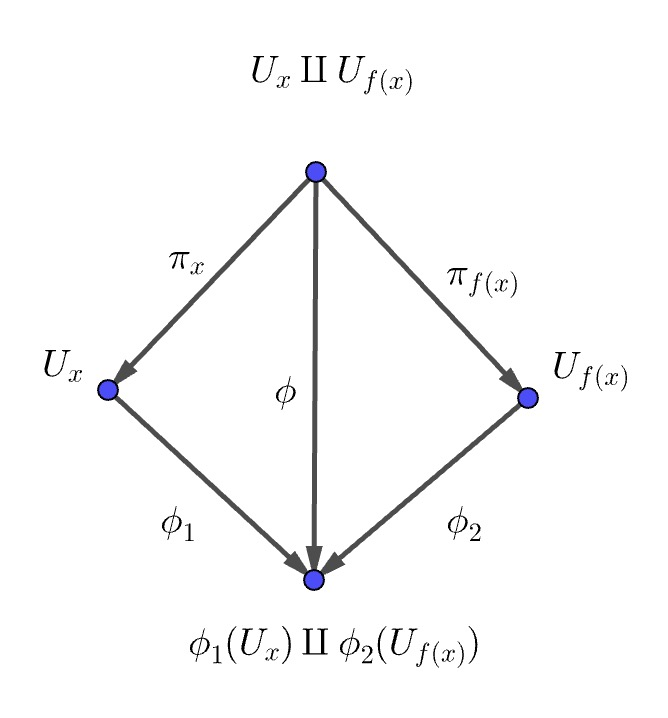
\includegraphics[scale=0.3]{Topology-Lee/image3.jpg}
                \caption{The diagram of $\phi$.}
                \label{fig:3}
            \end{figure}
            We will define $\phi' \colon U_x\cup_f U_{f(x)} \to \phi_1(U_x)\cup_\sim \phi_2(U_{f(x)})$ to be the continuous function such that the following diagram commute (yes again).
            \begin{figure}[H]
                \centering
                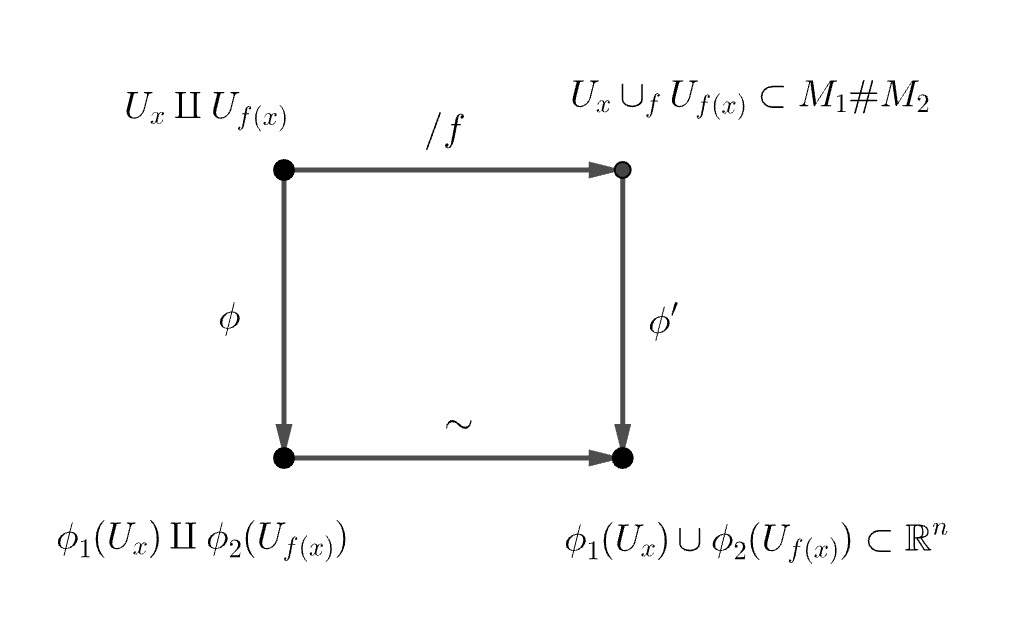
\includegraphics[scale = 0.3]{Topology-Lee/image4.jpg}
                \caption{The diagram of $\phi'$}
                \label{fig:4}
            \end{figure}

            Ok, where are we. We are showing that $x$ is locally Euclidean by finding a coordinate ball of $x=f(x)\in M_1'\amalg M_2'$ by looking for an open ball centered at $\phi(x)$ and take its inverse image over $\phi'$. Since we are in $\R^n$, we have something to grab on now, aka its metric. 
            Because $\phi_1(U_x)$ is open in $\Hs^n$, there exists $\epsilon_1>0$ such that $B_{\epsilon_1}(\phi_1(x))\cap \Hs^n$ is inside $\phi_1(U_x)$. Similarly, because $\phi_2(U_{f(x)})$ is open in $\Hs^n$, there exists $\epsilon_2 > 0$ such that $B_{\epsilon_2}(\phi_2(U_{f(x)})) \cap \Hs^n$ is inside $\phi_2(U_{f(x)})$. Let $\epsilon=\min\{\epsilon_1,\epsilon_2\}$, then $B:=B_\epsilon(\phi_1(x))=B_\epsilon(\phi_2(f(x)))$ is inside $\phi_1(U_x) \cup_\sim \phi_2(U_{f(x)})$, the quotient map just like in the Figure \ref{fig:2}. (There are two $\Hs^n$ used in this proof. They are different but share the same name. Let me know if it causes any confusion.) So the inverse image of this ball $B$ with respect to $\phi$ is a coordinate ball for $x$, aka $\phi^{-1}(B)$. 
            \begin{figure}[H]
                \centering
                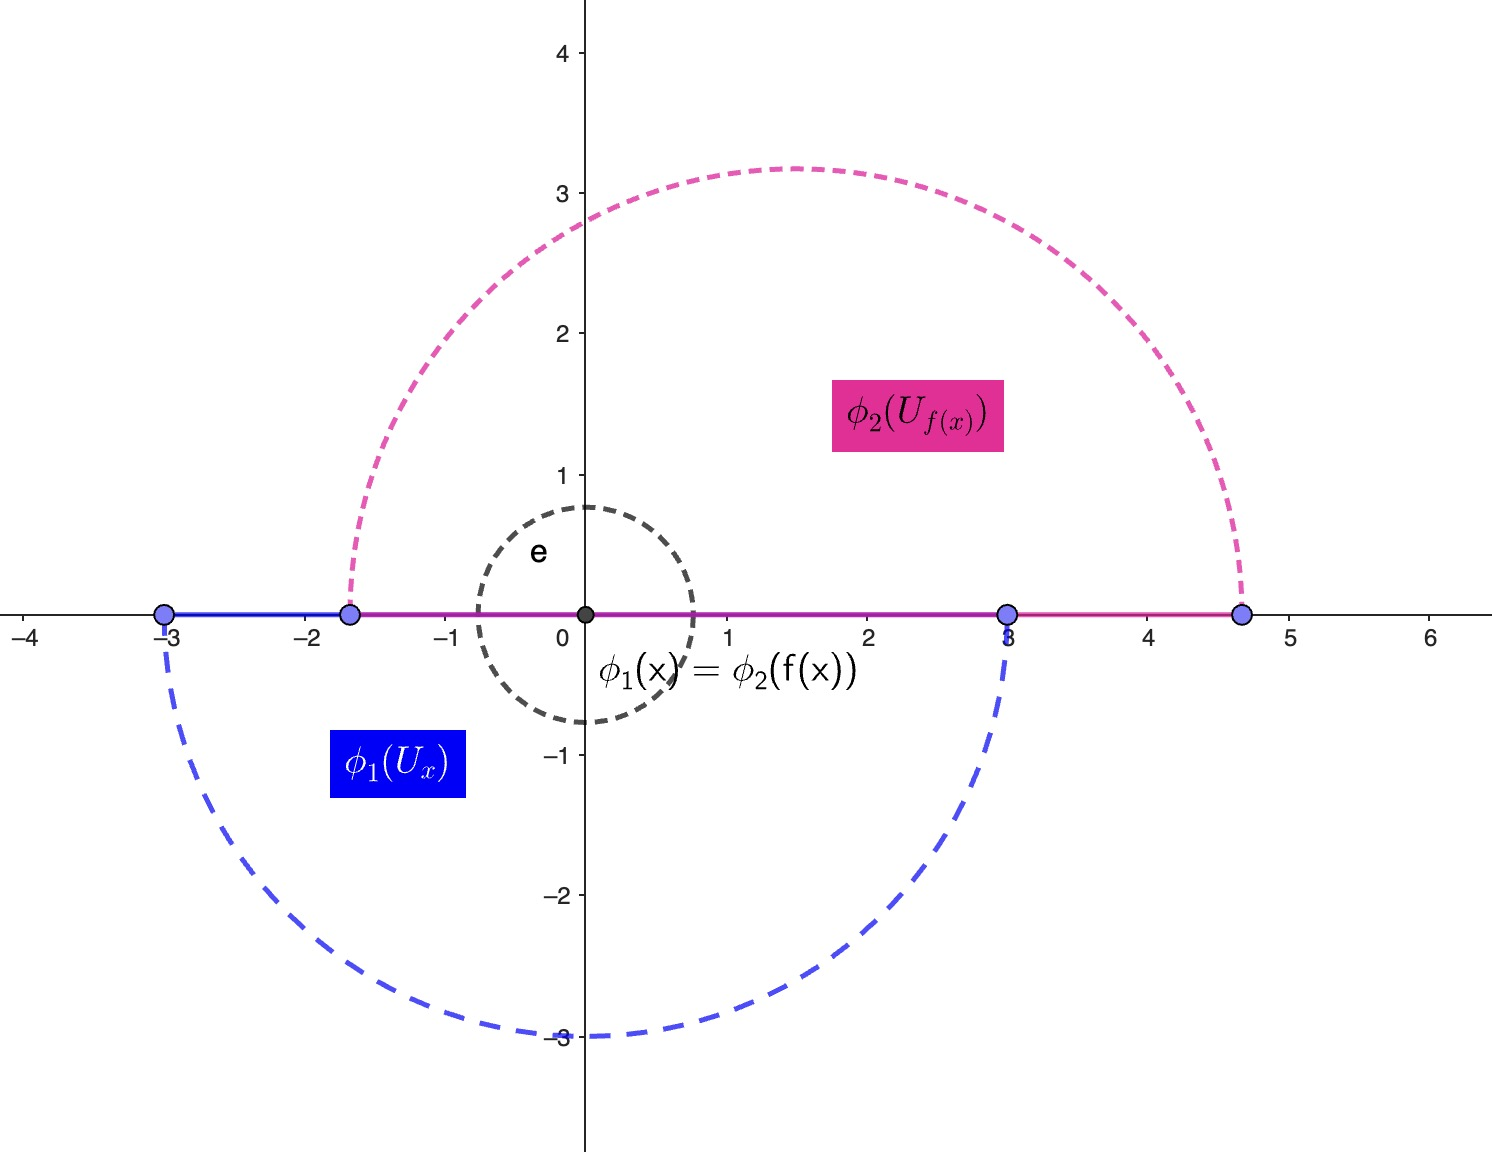
\includegraphics[scale=0.3]{Topology-Lee/image2.jpg}
                \caption{Our searching for $B$.}
                \label{fig:2}
            \end{figure}

            \item If $M_i'$ are connected, then because $M_1'$ and $M_2'$ shares the boundary in $M_1\# M_2$, $M_1\#M_2$ is also connected. Thus it is sufficient to prove that $M_i'$ are connected. Because $M_i$ is a manifold, it is locally connected. But $M_i$ is connected by the assumption, thus $M_i$ is path connected. We will now show that $M_i'$ is also path connected. For any $x,y\in M_i'$, since $M_i$ is path connected, there exists a continuous function $g\colon [0,1]\to M_i$ that maps $0\mapsto x$ and $1\mapsto y$. If this path, aka the image of $g$, does not pass $B_i$, then $g$ is a path from $x$ to $y$ in $M_i'$ and we are done. 
            
            Assume otherwise, that is $g([0,1])\cap B_i=\varnothing$, we will show that $g([0,1])\cap \partial B_i \neq\varnothing$ by mathematical contradiction. If $g([0,1])\cap \partial B_i = \varnothing$, then $g^{-1}(B_i) = g^{-1}(\overline{B_i})$. Since $g$ is continuous, $g^{-1}(B_i)$ is clopen in $[0,1]$. But $g^{-1}(B_i)$ can't be empty by our assumption and can't be $[0,1]$ because $g(0)\not\in B_i$, we get a contradiction. 

            Ok, so $g([0,1])\cap \partial B_i \neq\varnothing$. Let $a = \inf\{t\in[0,1]\mid g(t)\in \partial B_i\}$ and $b=\sup\{t\in [0,1]\mid g(t)\in \partial B_i\}$. If $a=b$, it is not hard to see that $g([0,1])\cap U_i=\varnothing$, which is impossible. So $[a,b]$ is a subinterval of $[0,1]$. Notice that for $n>1$, the boundary of $B_i'$ is $\mS^n$ is path connected. So we can find a continuous function $h:[a,b]\to \partial B_i'$ that maps $a\mapsto g(a)$ and $b\mapsto g(b)$. Now we will define a function $k:[0,1]\mapsto M_i\setminus B_i$ as the following.
            \[
            k(t) = \begin{cases}
                g(t) \textrm{ if } t\in [0,a]\cup [b,1],\\
                h(t) \textrm{ if } t\in (a,b).
            \end{cases}
            \]
            It is not hard to see that (yes again, or else this proof would be super long) $k$ is a continuous map from $[0,1]\to M_i\setminus U_i$ such that $k(0)=g(0)=x$ and $k(1)=g(1)=y$. So $M_i\setminus U_i = M_i'$ is path connected. And this complete our proof.

            \item Assume that $M_1$ and $M_2$ are compact, then $M_1'$ and $M_2'$ are closed subsets of a compact space, thus compact. So their disjoint union is also compact. Proposition 4.36 (e) says that every quotient of a compact space is compact, thus $M_1\# M_2$ is compact
            
        \end{enumerate}
    \end{proof}

\begin{problem}{4-20}
    Consider the topology on the set of integers described in Problem 2-17. Show that $\Z$ with this topology is limit point compact but not compact.
\end{problem}
    \begin{proof}
        Let $A$ be any infinite subset of $\Z$, and $n\in A$. Then $-n\in \Z$ is a limit point of $A$ because any neighborhood of $-n$ must also contain $n\in A$. Therefore, $\Z$ is limit point compact. However, this space is not compact because $U_i=\{-i,i\}$ is an open cover for $\Z$. It is not hard to see that any finite subcover of $\{U_i\}$ does not cover $\Z$.
    \end{proof}

\begin{problem}{4-22}
    Let $X = (\R\times \Z)/\sim$, where $\sim$ is the equivalence relation generated by $(x,n)\sim (x,m)$ for all $n,m\in\Z$ and all $x\neq 0$. Show that $X$ is locally compact but does not have a basis of precompact open subsets.
\end{problem}
    \begin{proof}
        For any $(x,z)\in \R\times \Z$, when $x\neq 0$, the second entry does not matter (after the quotient map). Therefore, we can label $(x,z)$ by $x$ when $x\neq 0$ and $0_z$ when $x=0$. We first show that $X$ is locally compact. For any $x\in X$, we consider two cases. If $x\neq 0$, then $B_{|x|/2}(x)$ is a parametric neighborhood of $x$. If $x=0_z$, then $B_1(0_z)$ is a neighborhood of $0_z$ (which is not hard to see) and it is inside $([-1,1]\times \Z)/\sim$. But $([-1,1]\times \Z)/\sim$ is compact by Tychonoff's theorem and the fact that the quotient of a compact set is compact. Therefore, $X$ is locally compact. 

        (You may ask wtf is $B_1(0_z)$ since there is no metric on X. Well, it is the image of the open ball on $\R$, which contain $0_z$, with respect to the quotient map. So $B_1(0_z)$ contains only one origin. The notation is wrong, but it is convenient and hopefully causes no confusion.)

        We now show that $X$ has no basis of a precompact open subset by showing that for any neighborhood $U$ of $0_1$, $\overline{U}$ cannot be compact. It is not hard to see that $\overline{U}$ must contain $\{0_z:z\in\Z\}$. However, let $U_z = \overline{U}\setminus \{0_t:t\neq z\}$ (the open sets that contain exactly one origin), then $\{U_z\}$ is an open cover for $\overline{U}$ that has no finite subcover. So $\overline{U}$ is not compact, which means $X$ has no precompact open basis.
    \end{proof}


\begin{problem}{4-23}
    Let $X$ be a locally compact Hausdorff space. The one-point compactification of $X$ is the topological space $X^*$ defined as follows. Let $\infty$ be some object not in $X$, and let $X^* = X\coprod\{\infty\}$ with the following topology:
    \[
    \T = \{\textrm{open subsets of $X$}\}\cup \{U\subset X^*:X^*\setminus U \textrm{ is a compact subset of $X$}\}.
    \]
    \begin{enumerate}[label=(\alph*)]
        \item Show that $\T$ is a topology.
        \item Show that $X^*$ is a compact Hausdorff space.
        \item Show that a sequence of points in $X$ diverges to infinity if and only if it converges to $\infty$ in $X^*$.
        \item Show that $X$ is open in $X^*$ and has the subspace topology.
        \item Show that $X$ is dense in $X^*$ if and only if $X$ is noncompact.
    \end{enumerate}
\end{problem}
    \begin{proof}
        \hfill
        \begin{enumerate}[label=(\alph*)]
            \item Because $\varnothing$ is open and compact, we get $\varnothing$ and $X^*$ to be elements of $\T$.
            Let $V_i$ be open subsets of $X$ and $U_i\subset X^*$ such that $X^*\setminus U$ is compact (thus $U_i$ contains $\infty$). Any arbitrary union $T$ of elements of $\T$ is the union of arbitrary many $U_i$ and $V_i$. If there is no $V_i$, then $T$ is open, thus $T\in \T$. Otherwise, we will consider $T^c$. We have
            \[
            T^c = \left(X^*\setminus\bigcup U_i\right)\setminus \bigcup V_i = \left(\bigcap X^*\setminus U_i \right)\setminus \bigcup V_i.
            \]
            Notice that the right-hand side is a compact set subtract an open set, which is again compact since $X$ is Hausdorff. Thus $T\in\T$. Lastly, any finite intersection $S$ of elements of $\T$ is a finite intersection of $U_i$ and $V_i$. Well, the finite case is easier by mathematical induction. Thus we only need to show that $U_1\cap U_2$, $V_1\cap V_2$ and $U_1\cap V_1$ are in $\T$. The first one is obvious. The second one is because
            \[
            X^*\setminus(V_1\cap V_2) = (X^*\setminus V_1)\cup (X^*\setminus V_2),
            \]
            which is the union of two compact sets, thus compact. For the last one, notice that $X$ is Hausdorff, thus $X^*\setminus U_1 = X\setminus U_1$ is closed. So $U_1\cap V_1$ is just an intersection of two open subsets, thus open. Mathematical induction implies that finite intersection of elements of $\T$ is in $\T$. So $\T$ defines a basis on $X^*$.

            \item We will show that $X^*$ is Hausdorff. For any $x,y\in X^*$, if both of them are in $X$ then we can easily separate them with open subsets of $X$. Let $y = \infty$, then using the locally compactness of $X$, we can find a neighborhood $V_x$ of $x$ that sits inside a compact subset $U$ of $X$. So $V_x$ and $X^*\setminus U$ are open subsets of $X^*$ that separate $x$ and $\infty$. So $X^*$ is Hausdorff.

            For the compactness, let $U_i$ be an arbitrary open cover for $X^*$, then without loss of generality, we assume that $\infty\in U_1$. So by the definition of $\T$, $X^*\setminus U_1 = X\setminus U_1$ is compact in $X$. Thus we can easily find a finite open subcover for $X\setminus U_1$. Adding $U_1$ into the subcover we just found, we get a finite subcover for $X^*$. So $X^*$ is compact.
            \item 
            \item Because $X$ is an open subset of $X$, it is an open set of $X^*$. To show that $X$ has a subspace topology, we only need to show that for any compact subset $U$ of $X$, $X\setminus U$ is open. But $X$ is Hausdorff, thus $U$ is closed and $U^c$ is open.
            \item Assume that $X$ is dense in $X^*$, then $\overline{X} = X^*$. So $X$ is not closed, and thus noncompact (because $X$ is Hausdorff). Conversely, if $X$ is noncompact, then $\overline{X}$ must be strictly larger than $X$. And how much can we add into $X$ here but $\infty$, so $\overline{X}=X^*$, which is synonymous to $X$ being dense in $X^*$.
        \end{enumerate}
    \end{proof}


\begin{problem}{4-24}
    Show that a topological space is a locally compact Hausdorff space if and only if it is homeomorphic to an open subset of a compact Hausdorff space.
\end{problem}
    \begin{proof}
        If $X$ is a locally compact Hausdorff space, then it is homeomorphic to $X\subset X^*$ as in Problem 4-23. And the previous problem also shows that $X^*$ is compact and $X$ is an open subset, so we are done. Conversely, assume that $X$ is homeomorphic to an open subset $A$ of a compact Hausdorff space $Y$, since locally compact and Hausdorff are topological properties, we only need to show that $A$ is locally compact and Hausdorff. Clearly, $A$ is Hausdorff because is a subspace of a Hausdorff space. For any $x\in A$, Lemma 4.65 implies that $x$ has a precompact neighborhood $V_x$ such that $\overline{V_x} \subset A$. So $A$ is locally compact.
    \end{proof}


\begin{problem}{4-25}
    Let $\sigma: \mS^n\setminus\{N\}\to \R^n$ be the stereographic projection, as defined in Example 3.21. Show that $\sigma$ extends to a homeomorphism of $\mS^n$ with the one-point compactification of $\R^n$. 
\end{problem}
    \begin{proof}
        Let $\sigma^*$ be an extension of $\sigma$ that maps $N\mapsto \infty$. It is left to show that $\sigma^*$ is a homeomorphism. We first note that $f$ is a bijection. Let $U$ be any open subset of $\R\cup\{\infty\}$, if $U$ does not contain $\infty$, then $(\sigma^{*})^{-1}(U)=\sigma^{-1}(U)$ is an open subset of $\mS^n$ (it is not hard to see). If $U$ contains $\infty$, then $U^c$ is compact, thus closed. So $$(\sigma^{*})^{-1}(U)^c = (\sigma^{*})^{-1}(U^c) = \sigma^{-1}(U^c)=\sigma^{-1}(U)^c.$$
        The first and last equations are because $\sigma$ and $\sigma^*$ are bijective. The middle equation is because $\infty\not\in U^c$. Notice that $\sigma^{-1}(U)^c$ is closed because $\sigma$ is continuous, we get $(\sigma^{*})^{-1}(U)$ to be open. So $\sigma^*$ is a continuous map. By the closed map lemma, $\sigma^*$ is a homeomorphism.
    \end{proof}


\pagebreak
\begin{problem}{4-26}
    Let $M$ be a compact manifold of positive dimension, and let $p\in M$. Show that $M$ is homeomorphic to the one-point compactification of $M\setminus \{p\}$.
\end{problem}
    \begin{proof}
        We first show that $M\setminus\{p\}$ is locally compact, and thus has the one-point compactification. For any point $x\in M$, $x\neq p$, because $M$ is Hausdorff, $x$ and $p$ can be separated by $U_x$ and $U_p$. Because $M$ has a basis of precompact open subsets, we can find a precompact neighborhood $V_x\subset U_x$ of $x$. Notice that $\overline{V_x}\subset \overline{U_x}\subset U_p^c$, we get $\overline{V_x}$ compact in $M\setminus\{p\}$. So $M\setminus\{p\}$ has the one-point compactification.
        
        Let $M^*$ be the one-point compactification of $M\setminus\{p\}$ and $f:M\to M^*$ that maps $p\mapsto \infty$ and $x\mapsto x$ whenever $x\neq p$. Clearly, $f$ is a bijection, it is left to check that $f$ is an open map. The strategy is identical to that of the previous problem. For any open subset $U$ of $M^*$, if $M$ does not contain $\infty$, then $f(U)$ is open by the subspace topology. If $U$ contains $\infty$, then $U^c$ is compact. Because $f$ is the identity map outside $\{p\}$, we get $f(U)^c=f(U^c)$, which is closed. So $f(U)$ is open, and therefore $f$ is an open map. This implies that $f$ is a homeomorphism.
    \end{proof}


\begin{problem}{4-29}
    Let $X$ be a complete metric space or a locally compact Hausdorff space. Show that every nonempty countable closed subset of $X$ contains at least one isolated point.
\end{problem}
    \begin{proof}
        Let $A$ be a nonempty countable closed subset of $X$ and assume that $A$ contains no isolated point, we will show that for any $a\in A$, $A\setminus\{a\}$ is open and dense in $A$. The open part is easy because a singleton is closed. Because $a$ is a limit point, any neighborhood $U_a$ of $a$ contains some elements of $A$ other than $a$. This implies that $a\in \overline{A\setminus\{a\}}$. So $\overline{A\setminus\{a\}}=A$ or $A\setminus\{a\}$ is dense in $A$. 

        Because $A$ is countable, Baire Category Theorem implies that 
        \[
        \bigcap_{a\in A}A\setminus \{a\} = \varnothing
        \]
        is dense in $A$. But this is impossible because $A$ is nonempty. So $A$ must contain at least one isolated point.
    \end{proof}

\begin{problem}{4-30}
    Prove the following generalization of the gluing lemma: suppose $X$ is a topological space and $\{A_\alpha\}$ is a locally finite closed cover of $X$. If for each $\alpha\in A$ we are given a continuous map $f_\alpha\colon X_\alpha\to Y$ such that $f_\alpha|_{X_\alpha\cap X_\beta}=f_\beta|_{X_\alpha\cap X_\beta}$ for all $\alpha$ and $\beta$, then there exists a unique continuous map $f\colon X\to Y$ whose restriction to each $X_\alpha$ is $f_\alpha$.  
\end{problem}

\begin{problem}{4-31}
    Suppose $X$ is Hausdorff, locally Euclidean of dimension $n$, and paracompact. Show that $X$ is an $n$-manifold if and only if it has countably many components, as follows.
    \begin{enumerate}[label=(\roman)]
        \item Show that it suffices to assume $X$ is connected.
        \item Show that $X$ has a locally finite cover $\U$ by precompact open sets that are $n$-manifolds.
        \item Choose an arbitrary nonempty $U_0\in \U$, and say a set $U'\in \U$ is \textbf{finitely connected to $U_0$} if there is a finite sequence $U_0,U_1,\cdots,U_k$ of sets in $\U$ such that $U_k=U'$ and $U_i\cap U_{i-1}\neq \varnothing$ for $i=1,\cdots,k$. Show that every element of $\U$ is finitely connected to $U_0$, and conclude that $\U$ is countable.
    \end{enumerate}
\end{problem}

\begin{problem}{4-32}
    Prove that every closed subspace of a paracompact space is paracompact.
\end{problem}

\begin{problem}{4-33}
    Suppose $X$ is a topological space with the property that for every open cover of $X$, there exists a partition of unity subordinate to it. Prove that $X$ is paracompact.
\end{problem}

\begin{problem}{4-34}
    Suppose $M$ is an $n$-manifold that admits an injective continuous map into $\R^k$ for some $k$. Show that $M$ admits a proper embedding into $\R^{k+1}$.
\end{problem}

\subsection{Bonus Problem}
\begin{problem}{1}
Construct a set B inside of the real line such that every uncountable subset of R meets both B and its complement.
\end{problem}


Let $U$ be an uncountable closed subset of $\R$, we will construct a subset of $U$ mimicking the construction of the Cantor set, therefore, this subset has the cardinatily of at least $c$. By doing that, first we will show that we can separate $U$ into two uncountable closed halves by an interval. But for doing so, we need to prove some lemmas first.

For any $t\in U$, we have $\{x\in U:x\leq t\}$ and $\{x\in U:x\geq t\}$ covers $U$, so at least one of the two sets is uncountable (or else its union is countable, which implies $U$ is countable). Notice that $\{x\in U:x\leq t\}=U\cap (-\infty,t]$, which is the intersection of two closed sets, thus closed. Similarly for $\{x\in U:x\geq t\}$. Define $U^+=\{t\in U: \{x\in U:x\geq t\}\text{ is uncountable }\}$ be the set of points where the right side of each point is uncountable. Similarly, we define $U^-=\{t\in U: \{x\in U:x\leq t\}\text{ is uncountable }\}$.

\begin{lemma}{1}
$U^+$ and $U^-$ are nonzero.
\end{lemma}
	\begin{proof}
	The proof is by mathematical contradiction. Assume that $U^-$ is empty, then for any $t\in U$, we have $\{x\in U:x\leq t\}$ is countable. If $U$ is bounded above, then because $U$ is closed, $\max U$ exists. Since $\max U\in U$, by our assumption, we get $U = \{x\in U:x\leq \max U\}$ is countable, contradiction. But if $U$ is not bounded above, then $(-\infty,n]\cap U$ is countable for any $n\in \N$ since we can always apply our hypothesis on some $t\in U$ such that $t>n$. So
	\[
	U = \amalg_{n\in\N}(-\infty,n]\cap U,
	\] 
	which is a countable union of countable sets, thus countable, contradiction. So $U^-$ is nonempty, and the case for $U^+$ is similar.
	\end{proof}
	
\begin{lemma}{2}
There exists $u_-,u_+\in U$ such that $(u_-,u_+)$ cuts $U$ into two closed uncountable halves. That is $U\cap (-\infty,u_-]$ and $U\cap [u_+,+\infty)$ are closed uncountable sets.
\end{lemma}
	\begin{proof}
	If $U^+\cap U^-=\varnothing$, then for any $t_-\in U^-$ and $t_+\in U^+$, because there is uncountably many point of $U$ smaller or equals $t_-$, but only countably many points of $U$ smaller or equal $t_+$, we get $t_+<t_-$. Because $U^+$ and $U^-$ are nonzero (Lemma 1), such $t_-\in U^-$ exists. So $U^+$ is bounded above by $t_-$ (similarly for $U^-$). Let $u_+ = \sup U^+$ and $u_- = \inf U^-$, because $U$ is closed, we get $u_+,u_-\in U$. If $u_+<u_-$, then we get $u_+\in U^+$ and $u_-\in U^-$. So $U\cap (-\infty, u_+]$ is countable because $u_+\notin U^-$. Similarly we get $U\cap [u_-,\infty)$ is countable. Thus
	\[
	U = (U\cap (-\infty, u_+])\cup (U\cap [u_-,\infty))
	\]    
	is countable, contradiction. If $u_+ = u_-=u$, then we will show that $u$ is in neither $U^+$ or $U^-$. Indeed, let $t_k\in U^+$ and $t_k\rightarrow u$, then because $t_k\notin U^-$, we have $U\cap (-\infty,t_k]$ is countable for all $k\in\N$. Therefore
	\[
	U\cap (-\infty,u] = \{u\}\cup \left(\bigcup_{k\in \N} U\cap (-\infty,t_k] \right)
	\]
	is countable. So there are countably many points before $u$, which yields $u\notin U^-$. The proof for $u\notin U^+$ is similar, contradiction since $U^+$ and $U^-$ covers $U$.
	
	If $U^+\cap U^-$ contains exactly $1$ element, then define $u$ as the previous case, we get $U^+\cap U^-=\{u\}$. If $(-\infty,u)\cap U$ and $(u,\infty)\cap U$ are closed, then consider $U_0 = U\setminus\{u\}$. We have $U_0$ to be closed, uncountable and $U_0^+\cap U_0^-=\varnothing$. So this become the previous case, which is a contradiction. Without lost of generality, assume that $(-\infty,u)\cap U$ is not closed, then there exists $t_k\in U^+\setminus\{u\}$ such that $t_k\rightarrow u$. Because $U^+\cap U^-=\{u\}$, we get $t_k\notin U^-$. So applying similar argument as the first case, we get $u\notin U^+$, contradiction.
	
	So $U^+\cap U^-$ contains more than $1$ element, let $u_-<u_+\in U^+\cap U^-$, then there are uncountably many points of $U$ before $(u_-,u_+)$ and after $(u_-,u_+)$. So $(u_-,u_+)$ has cut $U$ in half as desire.
	\end{proof}

\begin{problem}{(why 2)}
Let $U$ be an uncountable closed subset $\R$. Show that $\card (U)=c$.
\end{problem}
	\begin{proof}
	Because $U\subset \R$, there is an obvious injection from $U\rightarrow \ R$. So $\card(U)\leq c$. Now we will show that $\card(U)\geq c$ by construct a subset of $U$ that has the cardinality of $c$. Because $U$ is closed uncountable, there exists an interval $J_1$ as describe in Lemma 2. Let $I_1 = U\setminus J_1$, then $I_1$ contains two halves, both of which are closed uncountable set. Apply Lemma 2 again and again, we end up with a set $\Delta\subset U$. So any element of $\Delta$ can be defined uniquely by a sequence of going left or right (I can give more detail if you need, basically this is because $U$ is closed). Hence $\card(\Delta) = 2^{\aleph_0}=c$. So $\card (U)\geq c$. Using the Bernstein's Theorem, there exists a bijection from $U$ to $\R$, which implies $\card(U)=c$.
	\end{proof}
	
	
\begin{problem}{(why 1)}
Consider the class $\F$ of closed, uncountable subsets of $\R$. Show that $\F$ has the cardinality exactly equal to the continuum.
\end{problem}
	\begin{proof}
	Because the complement of a closed set of $\R$ is an open set, there is a natural bijection from the family of closed subsets of $\R$ to the class of open subsets of $\R$. But $\R$ is second countable, thus the class of open subsets of $\R$ has the cardinality of $2^\aleph_0 = c$. So $\text{card}(\F)\leq c$.
	
	Moreover, the map $\R\rightarrow \F$ maps $r\mapsto [r-1,r+1]$ is a surjection, therefore $c\leq \text{card}(\F)$. So $\text{card}(\F) = c$.
	\end{proof}
	

\begin{problem}{(Bernstein set)}
Construct the Bernstein set. (Where does Mr. Koberda use the fact that each closed uncountable subset of $\R$ has the cardinality of continuum?) 
\end{problem}
	\begin{proof}
	Let $c$ be the ordinal number of $\R$. Since we have showed that $\text{card}(\F)=c$, $\F$ can be described as $\F = \{A_\epsilon: \epsilon < c\}$. Now we will construct $B$ and $B^c$ by transfinite induction. Let $B_0=B_0^c=\varnothing$ (the little $c$ above $B_0$ is just a notation, not the compliment). For any $\delta<c$, we will will let
	\[
	B_\delta = \bigcup_{i<\delta}B_i \cup \min\left\{A_\delta\setminus \bigcup_{j<\delta}(B_j\cup B_j^c)\right\},
	\]
	and
	\[
	B_\delta^c = \bigcup_{i<\delta}B_i^c \cup \min\left\{A_\delta\setminus \bigcup_{j<\delta}(B_j\cup B_j^c) \setminus B_\delta \right\}.
	\]
	What we write above is basically adding the minimum of $A_\delta$ minus all the numbers that we have used. Such minimum exists because $A_\delta$ is well ordered. Notice that because $\delta < c$, 
	\[
	\text{card}\left(\bigcup_{j<\delta}(B_j\cup B_j^c)\right) = \delta +\delta < c + c = c.
	\]
	Here $c+c=c$ because $c$ is an infinite cardinal number. But $\text{card}(A_\delta)=c$, thus we have
	\[
	A_\delta\setminus \bigcup_{j<\delta}(B_j\cup B_j^c)\neq \varnothing.
	\]
	So $B = \bigcup_{\delta<c}B_\delta$ meets every closed uncountable subset of $\R$. \textit{(And this is where you questioned on.)} Similarly for $B^c$, we get $B$ is a Bernstein set!
	\end{proof}


\section{Cell Complexes}

\subsection{Exercise}

\begin{exercise}{5.3}
    Prove the preceding proposition. Suppose $X$ is a topological space whose topology is coherent with a family $\B$ of subspaces.
    \begin{enumerate}[label=(\alph*)]
        \item If $Y$ is another topological space, then a map $f\colon X\to Y$ is continuous if and only if $f|_B$ is continuous for every $B\in \B$.

        \item The map $\coprod_{B\in \B}B\to X$ induced by inclusion of each set $B\hookrightarrow X$ is a quotient map.
    \end{enumerate}
\end{exercise}

\begin{proof}
    \hfill
    \begin{enumerate}[label=(\alph*)]
        \item If $f$ is continuous, then obviously $f|_B$ is also continuous. Conversely, if that $f|_B$ is continuous for every $B\in\B$, then for any $U\subset Y$ open and $B\in\B$, we have
        \[
        f^{-1}(U)\cap B = (f|_B)^{-1}(U).
        \]
        Since the right hand side is open and $X$ is coherent with $\B$, $f^{-1}(U)$ is also open. So $f$ is continuous.

        \item Because $\B$ covers $X$, $f$ is surjective. We will show that $X$ has the quotient topology induced by $f\colon \coprod_{B\in\B}B\to X$ as described above. Because $X$ is coherent with $\B$, $U\subset X$ is open if and only if $U\cap B$ is open for all $B\in\B$, which is synonymous with saying 
        \[
        f^{-1}(U) = \bigcup_{B\in \B}U\cap B
        \]
        is open in $\coprod_{B\in\B}B$. So $f$ is a quotient map.
    \end{enumerate}
\end{proof}

\subsection{Problem}


\setcounter{section}{6}

\section{Homotopy and the Fundamental Group}

\subsection{Exercise}

\begin{exercise}{7.6}
    Let $B\subset \R^n$ be any convex set, $X$ be any topological space, and $A$ be any subset of $X$. Show that any two continuous maps $f,g\colon X\to B$ that agree on $A$ are homotopic relative to $A$.
\end{exercise}
    \begin{proof}
        Let $H:X\times I\to B$ defined by $H(x,t)=f(x)+t(g(x)-f(x))$. Example 7.4 shows that this is the straight-line homotopy between $f$ and $g$ (because $B$ is convex). Notice that for any $x\in A$, we get $f(x)=g(x)$. Thus $H(x,t)=f(x)=g(x)$ for all $x\in A$ and $t\in I$. So $f$ and $g$ are homotophic relative to $A$.
    \end{proof}


\begin{exercise}{7.8}
    Prove Proposition 7.7, that is, let $X$ be a topological space. For any points $p,q\in X$, path homotopy is an equivalence relation on the set of all paths in $X$ from $p$ to $q$.
\end{exercise}
    \begin{proof}
        Let $f,g,h:I\to X$ be paths from $p$ to $q$. First, we show that $f\sim f$. Let $H\colon I\times I\to X$ defined by $H(s,t)=f(s)$. It is not hard to check that $H$ is a homotopy. Moreover, $H(0,t)=f(0)=q$ and $H(1,t)=f(1)=q$. So $H$ is a path homotopy from $f$ to $f$.

        Second, we show that if $f\sim g$, then $g\sim f$. Assume that $f\sim g$, then there exists a path homotopy $H\colon I\times I\to X$ such that $H(s,0)=f(s)$ and $H(s,1)=g(s)$. Let $H'\colon I\times I\to X$ defined by $H'(s,t)=H(s,1-t)$. It is clear that $H$ is a homotopy between $g$ and $f$. Moreover, $H'(0,t)=H(0,1-t)=p$ and $H'(1,t)=H(1,1-t)=q$. So $H'$ is a path homotopy from $g$ to $f$.

        Third, we show that if $f\sim g$ and $g\sim h$, then $f\sim h$. Assume that $f\sim g$ and $g\sim h$, then there exist path homotopy $H,G\colon I\times I\to X$ between $f$ and $g$ and between $g$ and $h$ respectively. Let $F\colon I\times I\to X$ defined by 
        \[
        F(s,t)=\begin{cases}
            H(s,2t) & t\leq \frac{1}{2},\\
            G(s,2t-1) &  t\geq \frac{1}{2}.
        \end{cases}
        \]
        In Proposition 7.1, we have checked that $F$ is a homotopy between $f$ and $h$. What is more, because $H(0,t)=G(0,t)=p$, we get $F(0,t)=p$. Similarly, we get $F(1,t)=q$. This implies $F$ to be a path homotopy. So path homotopy defines an equivalence relation on the set of all paths from $p$ to $q$.
    \end{proof}


\begin{exercise}{7.14}
    Let $X$ be a path-connected topological space.
    \begin{enumerate}[label=(\alph*)]
        \item Let $f,g\colon I\to X$ be two paths from $p$ to $q$. Show that $f\sim g$ if and only if $f\cdot \bar g\sim c_p$.
        \item Show that $X$ is simply connected if and only if any two paths in $X$ with the same initial and terminal and points are path-homotopic.
    \end{enumerate}
\end{exercise}
    \begin{proof}
        \hfill
        \begin{enumerate}[label=(\alph*)]
            \item If $f\sim g$, then $[f]=[g]$. Thus $[f]\cdot [\bar g] = [f]\cdot [\bar f]=[c_p]$. Hence $f\cdot \bar g \sim c_p$. Conversely, if $f\cdot \bar g \sim c_p$, then $[f]\cdot [\bar g]=[c_p]$. Multiplying both sides on the right by $[g]$, we get $[f]=[g]$. Hence $[f]=[g]$.
            \item If $X$ is simply connected, then for any $p,q\in X$ and $f,g$ be two paths from $p$ to $q$. Clearly $f\cdot \bar g$ is a path from $p$ to $p$, thus $f\cdot \bar g\sim c_p$ because $X$ is simply connected. Part (a) implies that $f\sim g$. Conversely, if $f\sim g$ for any paths $f$ and $g$ as above, then we can let $p=q$. The hypothesis becomes any loop is path-homotopic to $c_p$. Thus $X$ is simply connected.
        \end{enumerate}
    \end{proof}


\begin{exercise}{7.15}
    Show that every convex subset of $\R^n$ is simply connected. Conclude that $\R^n$ itself is simply connected.
\end{exercise}
    \begin{proof}
        From Exercise 7.6, we know that any two continuous maps $f,g\colon X\to B$ that agree on $A\subset X$ are homotopic relative to $A$. Let $X=I$ and $A=\{0,1\}$. So any path $f,g\colon I\to B$ with same initial and terminal points are path-homotopic. Exercise 7.24(b) implies that $B$ is simply connected. Since $\R^n$ is convex, we get get $\R^n$ is simply connected.
    \end{proof}

\begin{exercise}{7.23}
    Prove that if $f_0,f_1\colon I\to X$ are path-homotopic and $\varphi\colon X\to Y$ is continuous, then $\varphi \circ f_0$ and $\varphi\circ f_1$ are path-homotopic.
\end{exercise}
    \begin{proof}
        Because $f_0$ and $f_1$ are path homotopic, they share the same initial point and terminal point. That means $\varphi\circ f_0$ and $\varphi\circ f_1$ share the same initial point and terminal point. Let $H\colon I\times I\to X$ be a path homotopy between $f_0$ and $f_1$, we define $H':= \varphi\circ H$. Thus
        \begin{align*}
            H'(0,t) &= \varphi(H(0,t))=\varphi(f_0(0))=\varphi(f_1(0));\\
            H'(1,t) &= \varphi(H(1,t))=\varphi(f_0(1))=\varphi(f_1(1));\\
            H'(s,0) &= \varphi(H(s,0))=\varphi(f_0(s));\\
            H'(s,1) &= \varphi(H(s,1))=\varphi(f_1(s)).
        \end{align*}
        These calculations guarantee that $\varphi \circ f_0$ and $\varphi\circ f_1$ are path-homotopic.
    \end{proof}

\begin{exercise}{7.27}
    Prove the following facts about retracts.
    \begin{enumerate}[label=(\alph*)]
        \item A retract of a connected space is connected.\\
        \item A retract of a compact space is compact.\\
        \item A retract of a retract is a retract; that is, if $A\subset B\subset X$, $A$ is a retract of $B$, and $B$ is a retract of $X$, then $A$ is a retract of $X$.
    \end{enumerate}
\end{exercise}
    \begin{proof}
    In part a) and b), let $A\subset X$ be a retract of $X$, and $r\colon X\to A$ be a retraction of $A$.
    \begin{enumerate}[label=(\alph*)]
        \item Because continuous map maps connected set to connected set, thus $X$ is connected implies $A$ is connected.
        \item Because continuous map maps compact set to compact set, $X$ is compact implies $A$ is compact.
        \item Let $r_B\colon X\to B$ and $r_A\colon B\to A$ be retraction, then $r:=r_A\circ r_B\colon X\to A$ is continuous. Moreover, for any $a\in A\subset B$, we have
        \[
        r(a) = r_A\circ r_B(a) = r_A(a)=a.
        \]
        So $r$ is a retraction, which implies $A$ is a retract of $X$.
    \end{enumerate}
    \end{proof}

\begin{exercise}{7.33}
    Prove that the circle is not a retract of the closed disk.
\end{exercise}
    \begin{proof}
        Notice that $\mS^1$ is not simply connected, but a closed disk is a convex subset of $\R^2$ thus simply connected. By Corollary 7.29, $\mS^1$ can't be a retract of a closed disk.
    \end{proof}

\begin{exercise}{7.36}
    Prove Proposition 7.35. That is, homotopy equivalence is an equivalence relation on the class of all topological spaces.
\end{exercise}
    \begin{proof}
        First, for any topological space $X$, $\Id_X$ is a homeomorphism from $X$ to itself. Thus $X\simeq X$. Second, if $X\simeq Y$, then there exist continuous maps $\varphi\colon X\to Y$ and $\psi\colon Y\to X$ such that $\varphi\circ \psi = \Id_Y$ and $\psi\circ \varphi = \Id_X$. So $\phi$ is a homotopy equivalence, which means $Y\simeq X$. Third, assume that $X\simeq Y$ and $Y\simeq Z$, then there exist $\varphi_1\colon X\to Y, \psi_1\colon Y\to X$ and $\varphi_2\colon Y\to Z, \psi_2\colon Z\to Y$ to be the homotopy equivalences. It is not hard to check that $\varphi_2\circ \varphi_1\colon X\to Z$ is a homotophy equivalence, where $\psi_1\circ \psi_2$ be the homotopy inverse of $\varphi_2\circ \varphi_1$. So $X\simeq Z$.
    \end{proof}

\begin{exercise}{7.42}
    Show that the following are equivalent:
    \begin{enumerate}[label=(\alph*)]
        \item $X$ is contractible.
        \item $X$ is homotopy equivalent to a one-point space.
        \item Each point of $X$ is a deformation retract of $X$,
    \end{enumerate}
\end{exercise}
    \begin{proof}
        % We show that (a) implies (b). If $X$ is contractible, then by the definition, $\Id_X$ is homotopic to a constant map, say $r\colon X\to \{a\}$. Notice that $\Id_X:X\to X$, thus $a\in X$. Let $\iota_a:\{a\}\hookrightarrow X$ be the projection from $\{a\}$ onto $X$. Because $a\in X$, $\iota_a\circ r = r$, which is homotopic to $\Id_X$. Conversely, $r\circ \iota_a:\{a\}\to \{a\}=\Id_{\{a\}}$. Thus $X$ and $\{a\}$ are homotopy equivalent. 

        % Next we show that (b) implies (c). Assume that $X$ is homotopy equivalent to a one-point space $\{a\}$. It is not hard to check that any two one-point spaces are homotopy equivalent, for any $x\in X$, $\{x\}$ is homotopy equivalent to $\{a\}$, thus homotopy equivalent to $X$. So $x$ is a deformation retraction of $X$.

        % Ok, so because $\{x\}$ is homotopy equivalent to $X$, there exist continuous maps $\phi\colon \{x\}\to X$ and $\psi\colon X\to \{x\}$ such that $$
        
        % Last, (c) implies (a) is obvious.
        We will show that (c) implies (b). If $r\colon X\to \{x\}\subset X$ is a deformation retraction, then $\iota_{x}\colon \{x\}\hookrightarrow X$ is a homotopy inverse of $r$. So $X$ is homotopy equivalent to a one point space.

        Next, we will show that (b) implies (a). If $X$ is homotopy equivalent to a one point space $\{a\}$, then there exist $\phi\colon X\to \{a\}$ and $\psi\colon \{a\}\to X$ such that $\psi\circ \phi$ is homotpic to $\Id_X$. Notice that the image of $\phi$ is a singleton, we get $\psi\circ \phi$ to be a constant map.

        Last, we will show that (a) implies (c). Since all constant maps are homotopic, if $X$ is contractible, then for any $x\in X$, the continuous map $r\colon X\to \{x\}$ is homotopic to $\Id_X$. Because $x\in X$, $\iota_x\circ r = r\simeq \Id_X$, where $\iota_x$ is the projection of $\{x\}$ onto $X$. This prove that $r$ is a deformation retraction of $X$, or $x$ is a deformation retract of $X$.
    \end{proof}


\pagebreak

\subsection{Problem}

\begin{problem}{7-4}
    Prove the Square Lemma. That is, let $F\colon I\times I\to X$ be a continuous map, and let $f,g,h,$ and $k$ be the paths in $X$ defined by
    \begin{align*}
        f(s) = F(s,0);\\
        g(s) = F(1,s);\\
        h(s) = F(0,s);\\
        k(s) = F(s,1).
    \end{align*}
    Prove that $f\cdot g\sim h\cdot k$.
\end{problem}
    \begin{proof}
        We will define two paths on $I\times I$ as follow. Let $p_1\colon I\to I\times I$ defined by
        \[
        p_1(s) = \begin{cases}
            (2s,0) & s\leq \frac{1}{2},\\
            (1,2s-1) & s\geq \frac{1}{2}.
        \end{cases}
        \]
        The gluing lemma guarantees that $p_1$ is continuos. Similarly, define 
        \[
        p_2(s) = \begin{cases}
            (0,2s) & s\leq \frac{1}{2},\\
            (2s-1,1) & s\geq \frac{1}{2}.
        \end{cases}
        \]
        \begin{figure}[h]
            \centering
            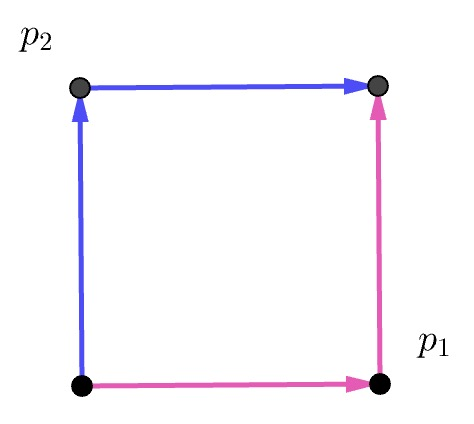
\includegraphics[scale = 0.3]{Topology-Lee/image6.jpg}
        \end{figure}

        Because $I\times I$ is a convex subset of $\R^2$ and $p_1$ and $p_2$ are paths with same initial and terminal points, they are path-homologic. So there exists a path-homotopy $H\colon I\times I \to I\times I$ between $p_1$ and $p_2$. We will show that $F\circ H$ is a path homotopy of $f\cdot g$ and $h\cdot k$. Clearly, $F\circ H$ is a composition of two continuous maps, thus continuous. What is more,
        \begin{align*}
            F\circ H(s,0) &= F(0,0) = f(0) = h(0);\\
            F\circ H(s,1) &= F(1,1) = f(1) = h(1);\\
            F\circ H(0,s) &= F(p_1(s))=\begin{cases}
            F(2s,0) & s\leq \frac{1}{2},\\
            F(1,2s-1) & s\geq \frac{1}{2}.
        \end{cases}\\&=\begin{cases}
            f(2s) & s\leq \frac{1}{2},\\
            g(2s-1) & s\geq \frac{1}{2}.
        \end{cases} = f\cdot g.\\
            F\circ H(1,s) & = h\cdot k \quad \text{ (similar as above)}.
        \end{align*}
        So $F\circ H$ is a path-homology between $f\cdot g$ and $h\cdot k$, which complete our proof.
    \end{proof}

\section{Circle}

\subsection{Exercise}


\subsection{Problem}



\setcounter{section}{10}
\section{Covering Maps}

\subsection{Exercise}

\begin{exercise}{11.2}
    Prove the following properties.
    \begin{enumerate}[label=(\alph*)]
        \item Every covering map is a local homeomorphism, and open maps, and a quotient map.
        \item An injective covering map is a homeomorphism.
        \item A finite product of covering maps is a covering map.
        \item The restriction of a covering map to a saturated, connected, open subset is a covering map onto its image.
    \end{enumerate}
\end{exercise}
    \begin{proof}
    Let $q\colon E\to X$ be a covering map.
    \begin{enumerate}[label=(\alph*)]
        \item For any point $e\in E$, there exists an evenly covering neighborhood $V_{f(e)}\subset X$ of $f(e)$. So there eixists a neighborhood $\tilde U$ of $e$ that is homeomorphic to $V_{f(e)}$, which shows that $q$ is a locally homeomorphism. From Proposition 2.31, $q$ is also an open map. Moreover, because $q$ is a surjective open map, Proposition 3.69 implies that $q$ is a quotient map.
        \item Since $q$ is injective and surjective, it is bijective. But every bijective local homeomorphism is a homeomorphism (Proposition 2.31), $q$ is a homeomorphism.
        \item We will prove that the product of two covering maps is a covering map. The finite part is by mathematical induction. Let $q_1\colon E_1\to X_1$ and $q_2\colon E_2\to X_2$ be covering maps. So $q_1\times q_2\colon E_1\times E_2\to X_1\to X_2$ maps $(a,b)\mapsto (q_1(a),q_2(b))$. Because any finite product of connected and locally path-connected set is connected and locally path connected, $E_1\times E_2$ is connected and locally path-connected.

        For any point $(e_1,e_2)\in E_1\times E_2$, let $U_1$ and $U_2$ be the evenly covers for $e_1$ and $e_2$. So
        \[
        q^{-1}_1(U_1) = \coprod_{i\in I} \tilde U_1(i),
        \]
        where $\tilde U_1(i)$ are open connected subset of $X_1$ that is homeomorphic to $U_1$. Similarly for
        \[
        q_2^{-1}(U_2) = \coprod_{i\in I'} \tilde U_2(i).
        \]
        It is not hard to check that for any $i,j\in I,I'$, we have $\tilde U_1(i)\times \tilde U_2(j)$ an open, connected subset of $E_1\times E_2$ that is homeomorphic to $U_1\times U_2$. Since $(q_1\times q_2)^{-1}(U_1\times U_2) = q_1^{-1}(U_1)\times q_2^{-1}(U_2)$, the previous calculation guarantees that $q_1\times q_2$ is a covering map.
        \item Let $A\subset X$ such that $q^{-1}(A)$ is a connected open subset, we will show that $q|_{q^{-1}(A)}$ is a covering mapping. From our assumptions, one can easily check that $q^{-1}(A)$ is also locally connected. Since $q$ is continuous, $A$ is open. So for any $a\in A$ and $U_a$ an evenly covered of $a$, we can find a connected neighborhood $U'_a\subset A\cap U_a$ of $a$. We claim that this is an evenly covered for $a$ by $q|_{q^{-1}(A)}$. Indeed, we have
        \[
        \left(q|_{q^{-1}(A)} \right)^{-1}(U'_a) = q^{-1}(A)\cap q^{-1}(U'_a) = q^{-1}(U'_a).
        \]
        The last equality is because $U'_a\subset A$. But $q^{-1}(U'_a)$ is a disjoint union of open connected subsets of $E$, each of which homeomorphic to $U'_a$ by $q$. Notice that $q^{-1}(U'_a)\subset q^{-1}(A)$, these components are homeomorphic to $U'_a$ by $q|_{q^{-1}(A)}$. So the restriction of a covering map to a saturated, connected, open subset is a covering map onto its image.
        
    \end{enumerate}
    
    \end{proof}

\begin{exercise}{11.9}
    Prove that the map $f$ in the preceding example is not a covering map by showing that the point $1\in\mS^1$ has no evenly covered neighborhood.
\end{exercise}
    \begin{proof}
        If there exists $U$ an evenly covered for $1$, then $f^{-1}(U)$ is a disjoint of connected components which is homeomorphic to $U$ by $f$. Notice that $f^{-1}(1) = \{1\}$, thus $f^{-1}(U)$ has one single component, therefore, $f^{-1}(U)$ homeomorphic to $U$ by $f$. But for any point $x\neq 1$, $f^{-1}(x)$ has at least two elements. Since $U$ is open, it is not a singleton. So $f|_U$ is not a bijection, contradiction. So $1\in\mS^1$ has no evenly covered neighborhood.
    \end{proof}

\begin{exercise}{11.25}
    Prove that if $S_1$ and $S_2$ are right $G$-sets and $\varphi\colon S_1\to S_2$ is a $G$-isomorphism, then $\varphi^{-1}$ is also a $G$-isomorphism.
\end{exercise}
    \begin{proof}
        Because $\varphi$ is a bijection, $\varphi^{-1}\colon S_2\to S_1$ is well-defined and bijective. It is sufficient to show that $\varphi^{-1}$ is also a $G$-equivariant. Indeed, for any $s\in S_2$ and $g\in G$, we have
        \[
        \varphi\circ \varphi^{-1}(sg) = sg = \varphi\circ \varphi^{-1}(s)g = \varphi(\varphi^{-1}(s)g).
        \]
        Notice that the last equality is because $\varphi$ is $G$-equivariant. Since $\varphi$ is a bijection, the equation above proves that 
        \[
        \varphi^{-1}(sg)=\varphi^{-1}(s)g.
        \]
        So $\varphi^{-1}$ is $G$-equivariant.
    \end{proof}



\subsection{Problem}


\begin{problem}{11-1}
    Suppose $q\colon E\to X$ is a covering map.
    \begin{enumerate}[label=(\alph*)]
        \item Show that if $X$ is Hausdorff, then $E$ is too.
        \item Show that if $X$ is an $n$-manifold, then $E$ is too.
        \item Show that if $E$ is an $n$-manifold and $X$ is Hausdorff, then $X$ is an $n$-manifold.
    \end{enumerate}
\end{problem}
    \begin{proof}
    \hfill
    \begin{enumerate}[label=(\alph*)]
        \item Assume that $X$ is Hausdorff. Let $e_1,e_1\in E$ and consider $q(e_1),q(e_2)\in X$. We can find neighborhoods $U_1$ and $U_2$ of $q(e_1),q(e_2)$ respectively such that $U_1\cap U_2 = \varnothing$ since $X$ is Hausdorff. Because $q$ is continuous, $q^{-1}(U_1)$ and $q^{-1}(U_2)$ are disjoint neighborhoods of $e_1$ and $e_2$, which shows that $E$ is Hausdorff.

        \item For any point $e\in E$, there is a neighborhood $U_e\subset E$ that is homeomorphic to $V_e\subset X$, an evenly covered of $q(e)$, by $q$. Because $X$ is locally Euclidean, we can find a coordinate ball $B$ of $q(e)$ that sits inside $V_e$. So $(q|_{U_e})^{-1}(B)$ is a coordinate ball of $e$, which prove that $E$ is locally Euclidean.

        Now we will show that $E$ is second countable. Let $\B$ be a countable basis for $X$. We will construct $\tilde{\B}$ as follows. For each $B\in \B$ such that $B$ is evenly covered, we have
        \[
        q^{-1}(B) = \bigcup_{i\in \N}\tilde B_i.
        \]
        The set $\tilde\B$ is defined to be the set of all such $\tilde B_i$. Since a countable union of countable sets is countable, $\tilde \B$ is countable. We show that $\tilde\B$ is indeed a basis for $E$. For any nonempty open subset $U\subset E$, let $e\in U$. Let $x = q(e)\in X$, and $V_x$ be an evenly covered neighborhood of $x$, we can find $\tilde V_x\subset E$  that is homeomorphic to $V_x$ by $q' = q|_{\tilde V_x}$ and containing $e$. Notice that $U\cap \tilde V_x$ is open in $E$, $q'(U\cap \tilde V_x)$ is open in $X$. Let $B\in \B$ be a subset of $q'(U\cap \tilde V_x)$, then there is a $\tilde B\in \tilde \B$ that is in $U\cap \tilde V_x\subset V_x$. So $\tilde \B$ is a basis for $E$.

        \item Let $\B$ be a countable basis for $E$, then $q(\B) = \{q(B)\mid B\in \B\}$ is clearly a countable basis for $X$. Since we already assume the Hausdorff property, we only need to check X is locally Euclidean. 

        For any $x\in X$, let $V_x$ be the evenly covered of $x$. Take a random point $x'\in q^{-1}(x)$ and $\tilde V_{x'}$ be a sheet of the covering over $V_x$ that contains $x'$. Since $E$ is locally Euclidean, we can find a coordinate ball $B_{x'}\subset \tilde V_{x'}$ of $x'$. Thus $q(B_{x'})$ is a coordinate ball of $x$, which proves that $X$ is locally Euclidean.
    \end{enumerate}
    \end{proof}

\pagebreak

\begin{problem}{11-11}
    Let $q\colon E\to X$ be a covering map. Show that $E$ is compact if and only if $X$ is compact and $q$ is a finite-sheeted covering.
\end{problem}
    \begin{proof}
        Assume that $E$ is compact, then because $q$ is continuous, $X$ is also compact. We now show that $q$ is a finite-sheeted covering by showing that a fiber of any point has to be finite. For each evenly covered set $U\subset X$, we have
        \[
        q^{-1}(U) = \bigcup_{i\in A}\tilde U_i,
        \]
        where $A$ is an index set. We define $\B$ to be the set of all such $\tilde U_i$. It is not hard to see that $\B$ is an open cover of $E$. Take any $x\in X$ and any $\tilde x_1,\tilde x_2\in q^{-1}(x)$. Because any element of $B$ homeomorphic to a subspace of $X$, it cannot contain both $\tilde x_1$ and $\tilde x_2$. That means, if $q^{-1}(x)$ has infinite elements, $E$ cannot be covered by a finite subcover of $\B$, which contradicts to $E$ being compact. So $q$ is a finite-sheeted covering.

        Conversely, assume that $X$ is compact and $q$ is a finite-sheeted covering, then because the set of evenly covered neighborhoods of $X$ covers $X$, $X$ is covered by evenly covered neighborhood $U_1,\cdots, U_n$. Then let
        \[
        q^{-1}(U_i) = \bigcup_{j\in D}\tilde U_{i}^{j}
        \]
        where $D$ is a finite index set, we can see that $\tilde U_{i}^{j}$ is compact for each $i,j$. And since $E$ is a finite union of compact sets $\tilde U_i^j$, we conclude that $E$ is compact.
    \end{proof} 


\begin{problem}{11-12}
    A continuous map $f\colon \mS^1\to \mS^1$ is said to be odd if $f(-z)=-f(z)$ for all $z\in \mS^1$, and even if $f(z)=f(-z)$ for all $z\in\mS^1$. Show that every odd map has odd degree, as follows.
    \begin{enumerate}[label=(\alph*)]
        \item Let $p_2\colon \mS^1\to \mS^1$ be the two-sheeted covering map of Example 11.4. Show that if $f$ is odd, there exists a continuous map $g\colon \mS^1\to \mS^1$ such that $\deg f=\deg g$ and the following dia
    \end{enumerate}
\end{problem}

\section{Group Actions and Covering Maps}


\pagebreak

\section{Homology}

\subsection{Exercise}

\begin{exercise}{13.10}
    Prove Corollary 13.9. That is, suppose $f\colon X\to Y$ is a homotopy equivalence. Then for each $p\geq 0$, $f_*\colon H_p(X)\to H_p(Y)$ is an isomorphism.
\end{exercise}
    \begin{proof}
        Assume that $f\colon X\to Y$ is a homotopy equivalence and $g\colon Y\to X$ is its homotopy inverse. Then by Theorem 13.8, we have
        \[
        f_*\circ g_* = (f\circ g)_* = (\Id_Y)_*.
        \]
        Similarly, we have $g_*\circ f_* = (\Id_X)_*$. Since $(\Id_X)_*$ and $(\Id_Y)_*$ are the identities, we get $f_*$ is an isomorphism.
    \end{proof}

\begin{exercise}{13.12}
    Show that if $F,G\colon C_*\to D_*$ are chain homotopic chain maps, then $F_*=G_*\colon H_p(C_*)\to H_p(D_*)$ for all $p$.
\end{exercise}
    \begin{proof}
        Assume that $h$ is a chain homotopy from $F$ to $G$, then we have the following commute diagram.
        % https://q.uiver.app/#q=WzAsMTAsWzEsMCwiQ197cCsxfSJdLFsyLDAsIkNfcCJdLFszLDAsIkNfe3AtMX0iXSxbMSwxLCJEX3twKzF9Il0sWzIsMSwiRF9wIl0sWzMsMSwiRF97cC0xfSJdLFswLDAsIlxcY2RvdHMiXSxbNCwwLCJcXGNkb3RzIl0sWzQsMSwiXFxjZG90cyJdLFswLDEsIlxcY2RvdHMiXSxbMCwxLCJcXHBhcnRpYWxfe3ArMX0iXSxbMSwyLCJcXHBhcnRpYWxfcCJdLFszLDQsIlxccGFydGlhbF97cCsxfSJdLFs0LDUsIlxccGFydGlhbF9wIl0sWzYsMF0sWzksM10sWzUsOF0sWzIsN10sWzEsMywiaCIsMV0sWzIsNCwiaCIsMV1d
\[\begin{tikzcd}
	\cdots & {C_{p+1}} & {C_p} & {C_{p-1}} & \cdots \\
	\cdots & {D_{p+1}} & {D_p} & {D_{p-1}} & \cdots
	\arrow["{\partial_{p+1}}", from=1-2, to=1-3]
	\arrow["{\partial_p}", from=1-3, to=1-4]
	\arrow["{\partial_{p+1}}", from=2-2, to=2-3]
	\arrow["{\partial_p}", from=2-3, to=2-4]
	\arrow[from=1-1, to=1-2]
	\arrow[from=2-1, to=2-2]
	\arrow[from=2-4, to=2-5]
	\arrow[from=1-4, to=1-5]
	\arrow["h"{description}, from=1-3, to=2-2]
	\arrow["h"{description}, from=1-4, to=2-3]
\end{tikzcd}\]

    An element of $H_p(C_*)$ has the form $\sigma+\im \partial_{p+1}$, where $\sigma\in \Ker\partial_p$. We will show that $F(\sigma +\im \partial_{p+1}) = G(\sigma+\im \partial_{p+1})$ by showing that $F(\sigma)-G(\sigma)\in \im \partial_{p+1}$ (Notice that the second $\partial_{p+1}$ is in $D_*$). Indeed, we have
    \[
    F(\sigma)-G(\sigma) = \partial_{p+1} \circ h(\sigma)+h\circ \partial_{p}\sigma = \partial_{p+1}\circ h(\sigma)\in \im \partial_{p+1}.
    \]
    So $F_*=G_*$.
    \end{proof}



\subsection{Problem}

\subsection{Bonus Problem}

\begin{problem}{1}
    Reproving Proposition 13.5.
\end{problem}
    \begin{proof}
        Our proof follows this equation.
        \[
        H_p(X) = \frac{Z_p(X)}{B_p(X)} \cong \frac{\bigoplus_{a\in A}Z_p(X_a)}{\bigoplus_{a\in A}B_p(X_a)} \cong \bigoplus_{a\in A}\frac{Z_p(X_a)}{B_p(X_a)}.
        \]
        The first and the last equations are by the definition of the homotopy group and by Claim 8.4 in Aluffi (lol). So we only need to prove the second isomorphism.

        First, we show that $C_p(X)\cong\bigoplus_{a\in A}C_p(X_a)$. Because $\Delta_p$ is path connected, any singular $p$-simplex of $X$ must be contained in some path component $X_a$. So we can write 
        \[
        C_p(X) = \langle{\{S_a\}_{a\in A}\mid \{R_a\}_{a\in A}}\rangle,
        \]
        where $C_p(X_a) = \langle{S_a\mid R_a}\rangle$ for each $a\in A$. And we are considering free abelian groups only. So $C_p(X)$ is isomorphic to $\bigoplus_{a\in A}C_p(X_a)$ under the natural isomorphism $\phi_p$ that take each generator to itself. Consider the following commutative diagram.
        % https://q.uiver.app/#q=WzAsNCxbMCwwLCJcXGJpZ29wbHVzX3thXFxpbiBBfUNfcChYX2EpIl0sWzAsMSwiQ19wKFgpIl0sWzIsMCwiXFxiaWdvcGx1c197YVxcaW4gQX1DX3twLTF9KFhfYSkiXSxbMiwxLCJDX3twLTF9KFgpIl0sWzEsMywiXFxwYXJ0aWFsIl0sWzAsMiwiXFxwYXJ0aWFsIl0sWzAsMSwiXFx2YXJwaGlfcCJdLFsyLDMsIlxcdmFycGhpX3twLTF9IiwyXV0=
\[\begin{tikzcd}
	{\bigoplus_{a\in A}C_p(X_a)} && {\bigoplus_{a\in A}C_{p-1}(X_a)} \\
	{C_p(X)} && {C_{p-1}(X)}
	\arrow["\partial", from=2-1, to=2-3]
	\arrow["\partial^A", from=1-1, to=1-3]
	\arrow["{\varphi_p}", from=1-1, to=2-1]
	\arrow["{\varphi_{p-1}}"', from=1-3, to=2-3]
\end{tikzcd}\]
        
        We will prove that $Z_p(X) \cong \bigoplus_{a\in A}Z_p(X_a)$ by showing that $\ker(\partial^A)\cong \ker(\partial)$ over $\phi_p$. But this is not hard to see since both $\varphi_p$ and $\varphi_{p-1}$ are isomorphism. Similarly, we can show that $B_p(X) \cong \bigoplus_{a\in A}B_p(X_a)$ by replacing $\ker$ with $\text{im}$ and $p$ with $p+1$. So Proposition 13.5 is proved.

        
    \end{proof}

\end{document}
